% ========================================= TEMPLATE INFO ========================================
%
% Author:       P4ntomime
% Version:      1.0.0
% Last updated: 2024-02-18
% Brief:        A LaTeX template for summaries. See README.md for more information.
% 
% ================================================================================================
\documentclass[8pt, a4paper, twoside]{extarticle}
% Font size:    8pt
% Paper size:   A4
% style:        twoside (needed, so odd and even pages have different margins)
% orientation:  portrait. (use 'landscape' for landscape orientation)


% ========================================= DOCUMENT INFO =========================================
\def\title{Signale und Systeme 2}                                   % title
\def\shorttitle{SigSys 2}                                           % short title (displayed as PDF title)
\def\dozent{Prof. Dr. Heinz Mathis}                                 % lecturer
\def\semester{FS 24}                                                % semester
\def\author{Simone Stitz, Laurin Heitzer}                           % author(s)
\def\repo{https://github.com/P4ntomime/signale-und-systeme-2}       % repository link
\def\version{1.0.\today}                                            % version
\def\pagelimit{100}                                                 % page limit -> causes pages after limit to be red


% ================================= PACKAGES, SETUP AND COMMANDS ==================================
% =========================================== PACKAGES ============================================
\usepackage[utf8]{inputenc}         % input encoding: UTF-8
\usepackage[T1]{fontenc}            % font encoding: T1
\usepackage{textcomp}               % additional symbols
\usepackage{times}                  % times new roman font
\usepackage[main=ngerman]{babel}    % set main language to german


\usepackage{multicol}               % provides multicols environment
\usepackage{geometry}               % set page layout


\usepackage{enumitem}               % list customization
\usepackage{outlines}               % easy nested lists
\usepackage{tabularx}               % some nicer tables with X columns
\usepackage{booktabs}               % booktabs seplines
\usepackage{hhline}                 % double lines in tables
\usepackage{boldline}               % bold (vertical) lines in tables


\usepackage{amsmath}                % math symbols
\usepackage{amssymb}                % more math symbols
\usepackage{empheq}                 % math boxes
\usepackage{mathtools}
\usepackage{mhsetup}
\usepackage{txfonts}
\usepackage[squaren]{SIunits}       % SI-units
\usepackage{bm}                     % bold math symbols
\usepackage{trfsigns}               % needed for "Laplace" symbol (Korrespondenz)
\usepackage{mathrsfs}               % needed for Fourier transform "F"


\usepackage{graphicx}               % include graphics
\usepackage{graphbox}               % needed for aligning images in multicol environment
\usepackage{scalerel}               % scale any objects
\usepackage{anyfontsize}            % set any font size
\usepackage[table]{xcolor}          % needed for colors


\usepackage{tcolorbox}              % colored boxes
\usepackage{contour}                % contour for text (used in custom underline command)
\usepackage[normalem]{ulem}         % custom underline (used in custom underline command)


\usepackage{tikz}                   % needed for TikZ drawings
\usetikzlibrary{angles}             % for the angle pic
\usetikzlibrary{positioning}        % for the positioning of the nodes
\usetikzlibrary{arrows}             % for the arrow tip
\usetikzlibrary{shapes.misc}        % for the cross out node shape

\usepackage{pgfplots}               % needed for  easy axis generation in TikZ drawings

\usepackage{listings}               % for nicer code display
% to use nodes inside listing see: https://texample.net/tikz/examples/tikz-listings/
\usepackage{inconsolata}            % consolas font for listings and text

\usepackage{hyperref}               % clickable links
\usepackage{qrcode}                 % QR code generation (also clickable)


\usepackage{ifthen}                 % if-then-else commands
\usepackage{calc}                   % simple arithmetic in LaTeX commands


\usepackage{draftwatermark}         % watermark on pages after a certain limit
\usepackage{fancyhdr}               % custom header and footer
\usepackage[explicit]{titlesec}     % custom section titles


\usepackage{datetime2}              % custom date format for versioning

% ========================================== BASIC SETUP ==========================================

% --------------------------------------- DOCUMENT SETTINGS ---------------------------------------
\hypersetup{hidelinks,
% set pdf metadata
            pdfauthor={\author},
            pdftitle={\shorttitle},
            pdfsubject={\title\ \semester},
            pdfkeywords={Gahn go lerne!!}}

% set style for URLs
\urlstyle{same} % sets url font to the same as the preceeding text

% set page layout
\geometry{left=3mm, 
          right=3mm, 
          top=3mm, 
          bottom=6mm, 
          headheight=0mm, 
          headsep=0mm, 
          footskip=4mm}

\setlength{\columnsep}{1.5mm}       % distance between columns
\setlength{\columnseprule}{0.1pt}   % thickness of column separation line
\setlength{\parindent}{0pt}         % no paragraph indentation

\setcounter{tocdepth}{2}            % only display sections and subsections in toc
% \setcounter{secnumdepth}{0}       % uncomment to disable section numbering

\DeclareMathSizes{8}{8}{6}{5}       % set math font sizes for 8pt document


% --------------------------------------- COLOR DEFINITIONS ---------------------------------------
\definecolor{sectioncolor}{HTML}{2EEBBF}
\definecolor{subsectioncolor}{HTML}{ABF7E5}
\definecolor{sectextcol}{HTML}{000000}
\definecolor{subsectextcol}{HTML}{000000}

\definecolor{backcolour}{HTML}{f5f5f0} % background color for highlighted text

% TODO: define color palette
% color palette: https://colorkit.co/color-palette-generator/FF8552-9e22bd-404E7C-C32E15-225A28/
\definecolor{green}{HTML}{11dd12}
\definecolor{red}{HTML}{f90d09}
\definecolor{blue}{HTML}{093ce5}
\definecolor{orange}{HTML}{f79300}
\definecolor{violet}{HTML}{a516c9}

% colors for listings (code)
\definecolor{commentcolour}{HTML}{008000}
\definecolor{keywordcolour}{HTML}{7f0055}
\definecolor{stringcolour}{HTML}{9e22bd}
\definecolor{numbercolour}{HTML}{808080}


% ----------------------------------- LIST AND TABULAR SETTINGS -----------------------------------
\setlist[enumerate]{label=\bfseries\arabic*.,   % label style bold arabic numerals (1., 2., ...)
                    leftmargin=*}               % remove left margin from enumerate
\setlist[itemize]{leftmargin=1.5em}             % left margin for itemize: 1.5em
\setlist{nosep}                                 % no vertical spacing between list items

\renewcommand{\arraystretch}{1}               % stretch table rows


% ----------------------------------- TIKZ / PGFPLOTS SETTINGS ------------------------------------
\usetikzlibrary{arrows}
\usetikzlibrary{arrows.meta}
\usetikzlibrary{bending}
\usetikzlibrary{decorations.pathreplacing}
\usetikzlibrary{angles}
\usetikzlibrary{tikzmark}
\usetikzlibrary{petri}
\usetikzlibrary{positioning}
\usetikzlibrary{shapes}
\usetikzlibrary{calc}

\pgfplotsset{compat=1.17}	        % newest version
\AtBeginEnvironment{tikzpicture}{\tracinglostchars=0\relax}

% ------------------------------------ OTHER PACKAGE SETTINGS -------------------------------------

% define and set new date style for versioning as YYYYMMDD
\DTMnewdatestyle{vnumdate}{%
    \renewcommand{\DTMdisplaydate}[4]{\number##1\DTMtwodigits{##2}\DTMtwodigits{##3}}%
    \renewcommand{\DTMDisplaydate}{\DTMdisplaydate}%
}
\DTMsetdatestyle{vnumdate}


% setup for ulem and contour packages
\renewcommand{\ULdepth}{1.75pt} % set underline depth
\contourlength{0.7pt}           % set contour length


% ====================================== SETUP AND COMMANDS =======================================

% custom underline command for exclusions on lowercase letters such as g, j, p, q, y
\newcommand{\myul}[1]{%
    \uline{\phantom{#1}}%
    \llap{\contour*{white}{#1}}%
}

% cunstom command for writing const correctly in math environment
\newcommand{\const}{%
    \mathrm{const}
}

% cunstom command for writing Dek correctly in math environment
\newcommand{\Dek}{%
    \mathrm{Dek}
}

% setup header and footer
\pagestyle{fancy}
\fancyhf{}                          % clear all header and footer fields
\renewcommand{\headrulewidth}{0pt}  % remove header rule
\renewcommand{\footrulewidth}{0pt}  % remove footer rule
\fancyfoot[C]{\thepage}             % page number in center of footer


% --------------------------------------- TITLE FORMATTING ----------------------------------------

% section formatting
\titleformat{\section}
            % {\fontsize{9}{8}\selectfont\bfseries}
            {\Large\bfseries}
            {}
            {0mm}
            {\tikz{
                \node[fill=sectioncolor,            % fill color:       sectioncolor
                      text=sectextcol,              % text color:       sectextcol
                      text width=\columnwidth-4pt,  % text width:       columnwidth - 2x padding
                      text depth=0pt,               % text depth:       0pt (needed so text stays vertically centered)
                      minimum height=5mm,           % minimum height:   5mm
                      inner sep=2pt,                % inner padding:    2pt
                      align=left]                   % text alignment:   left
                      {\thesection\ #1};}}

\titleformat{numberless, name=\section}
            % {\fontsize{9}{8}\selectfont\bfseries}
            {\Large\bfseries}
            {}
            {0mm}
            {\tikz{
                \node[fill=sectioncolor,            % fill color:       sectioncolor
                      text=sectextcol,              % text color:       sectextcol
                      text width=\columnwidth-4pt,  % text width:       columnwidth - 2x padding
                      text depth=0pt,               % text depth:       0pt (needed so text stays vertically centered)
                      minimum height=5mm,           % minimum height:   5mm
                      inner sep=2pt,                % inner padding:    2pt
                      align=left]                   % text alignment:   left
                      {#1};}}

\titlespacing{\section}
             {0mm}
             {1ex}
             {.5ex}


% subsection formatting
\titleformat{\subsection}
            {\large\bfseries}
            {}
            {0mm}
            {\phantomsection\tikz{
                \node[fill=subsectioncolor,         % fill color:       subsectioncolor 
                      text=subsectextcol,           % text color:       subsectextcol 
                      text width=\columnwidth-4pt,  % text width:       columnwidth - 2x padding 
                      text depth=0pt,               % text depth:       0pt (needed so text stays vertically centered)
                      minimum height=5mm,           % minimum height:   5mm 
                      inner sep=2pt,                % inner padding:    2pt 
                      align=left]                   % text alignment:   left
                      {\thesubsection\ #1};}}

\titleformat{numberless, name=\subsection}
            {\large\bfseries}
            {}
            {0mm}
            {\phantomsection\tikz{
                \node[fill=subsectioncolor,         % fill color:       subsectioncolor 
                      text=subsectextcol,           % text color:       subsectextcol 
                      text width=\columnwidth-4pt,  % text width:       columnwidth - 2x padding 
                      minimum height=5mm,           % minimum height:   5mm 
                      inner sep=2pt,                % inner padding:    2pt 
                      align=left]                   % text alignment:   left
                      {#1};}}

\titlespacing{\subsection}
             {0mm}
             {1ex}
             {.5ex}


% subsubsection formatting
\titleformat{\subsubsection}
            {\fontsize{10}{9}\selectfont\bfseries}
            % {\normalsize\bfseries}
            {\myul{\thesubsubsection{} }}
            {0mm}
            {\phantomsection{}\myul{#1}}

\titlespacing{\subsubsection}
             {0mm}
             {1.2ex}
             {.5ex}


% custom command for examples
\newcommand{\example}[1]{\subsubsection*{Beispiel: #1}}


% ----------------------------------- CUSTOM TABULAR SPECIFIERS -----------------------------------

% centered fixed width column type
\newcolumntype{P}[1]{>{\centering\arraybackslash}p{#1}}

% centered variable width column type
\newcolumntype{C}{>{\centering\arraybackslash}X}

% centered math column type
\newcolumntype{M}{>{$}c<{$}}

% left aligned math column type
\newcolumntype{O}{>{$}l<{$}}


% inline tikz node for later referencing
\newcommand{\tikznode}[2]{% from https://tex.stackexchange.com/a/402466/121799
	\ifmmode%
	\tikz[remember picture,baseline= (#1.base),inner sep=0pt] \node(#1){$#2$};
	\else
	\tikz[remember picture,baseline= (#1.base),inner sep=0pt] \node(#1){#2};
	\fi}


% custom inline tcolorbox
\newtcbox{\mybox}
            [1]
            [backcolour]
            {on line,
            arc=0pt,
            outer arc=0pt,
            colback=#1,
            colframe=#1,
            boxsep=0pt,
            left=1pt,
            right=1pt,
            top=1pt,
            bottom=1pt,
            boxrule=0pt}


\makeatletter

% ------------------------------- SECTIONING COMMANDS CUSTOMIZATION -------------------------------

% section: add optional argument to command for script page numbers
\let\old@sec\section%
\RenewDocumentCommand{\section}{somg}{%
    \IfBooleanTF{#1}{
        \IfNoValueTF{#2}{
            \IfNoValueTF{#4}{
                \old@sec*{#3}
            }{
                \old@sec*{#3 {\small(S. #4)}}
            }
        }{
            \IfNoValueTF{#4}{
                \old@sec*[#2]{#3}
            }{
                \old@sec*[#2]{#3 {\small(S. #4)}}
            }
        }%
    }{
        \IfNoValueTF{#2}{
            \IfNoValueTF{#4}{
                \old@sec{#3}
            }{
                \old@sec{#3 {\small(S. #4)}}
            }
        }{
            \IfNoValueTF{#4}{
                \old@sec[#2]{#3}
            }{
                \old@sec[#2]{#3 {\small(S. #4)}}
            }
        }%
    }
}


% subsection: add optional argument to command for script page numbers
\let\old@subsec\subsection%
\RenewDocumentCommand{\subsection}{somg}{%
    \IfBooleanTF{#1}{
        \IfNoValueTF{#2}{
            \IfNoValueTF{#4}{
                \old@subsec*{#3}
            }{
                \old@subsec*{#3 {\small(S. #4)}}
            }
        }{
            \IfNoValueTF{#4}{
                \old@subsec*[#2]{#3}
            }{
                \old@subsec*[#2]{#3 {\small(S. #4)}}
            }
        }%
    }{
        \IfNoValueTF{#2}{
            \IfNoValueTF{#4}{
                \old@subsec{#3}
            }{
                \old@subsec{#3 {\small(S. #4)}}
            }
        }{
            \IfNoValueTF{#4}{
                \old@subsec[#2]{#3}
            }{
                \old@subsec[#2]{#3 {\small(S. #4)}}
            }
        }%
    }
}


% subsubsection: add optional argument to command for script page numbers
\let\old@subsubsec\subsubsection%
\RenewDocumentCommand{\subsubsection}{somg}{%
    \IfBooleanTF{#1}{
        \IfNoValueTF{#2}{
            \IfNoValueTF{#4}{
                \old@subsubsec*{#3}
            }{
                \old@subsubsec*{#3 {\small(S. #4)}}
            }
        }{
            \IfNoValueTF{#4}{
                \old@subsubsec*[#2]{#3}
            }{
                \old@subsubsec*[#2]{#3 {\small(S. #4)}}
            }
        }%
    }{
        \IfNoValueTF{#2}{
            \IfNoValueTF{#4}{
                \old@subsubsec{#3}
            }{
                \old@subsubsec{#3 {\small(S. #4)}}
            }
        }{
            \IfNoValueTF{#4}{
                \old@subsubsec[#2]{#3}
            }{
                \old@subsubsec[#2]{#3 {\small(S. #4)}}
            }
        }%
    }
}


% custom text rightarrow to match tikz arrows
\renewrobustcmd{\textrightarrow}{%
    \tikz{%
        \draw[-{Stealth[length=1.7mm]},
              double]
                (0,0) to (0.3,0);}}

% custom text leftrightarrow to match tikz arrows
\newrobustcmd{\textlrarrow}{%
    \tikz{%
        \draw[{Stealth[length=1.7mm]}-{Stealth[length=1.7mm]},
              double]
                (0,0) to (0.4,0);}}


% custom command for size matched colored brackets
\newcommand{\bbr}[2]{\colorlet{saved}{.}\color{#1}\left(\color{saved}#2\color{#1}\right)\color{saved}}


% custom command for differential operator d
\newcommand{\diff}{\ensuremath{\mathop{} \! \mathrm{d}}}

% custom command for underset limes operator
\newcommand{\limes}[1]{\ensuremath{\underset{#1}{\lim}}}

% custom command for absolute value
\newcommand{\abs}[1]{\ensuremath{\left|#1\right|}}

% custom command for imaginary unit, j
\newcommand{\jimg}{\ensuremath{\mathrm{j}}}

% custom command for real parts with argument
% \renewcommand{\Re}[1]{\ensuremath{\operatorname{Re}\left\lgroup#1\right\rgroup}}
\renewcommand{\Re}[1]{\ensuremath{\operatorname{Re}\left\{#1\right\}}}

% custom command for imaginary parts with argument
% \renewcommand{\Im}[1]{\ensuremath{\operatorname{Im}\left\lgroup#1\right\rgroup}}
\renewcommand{\Im}[1]{\ensuremath{\operatorname{Im}\left\{#1\right\}}}

% custom command for upper-case roman numbers with argument
\newcommand{\uproman}[1]{\uppercase\expandafter{\romannumeral#1}}

% shortcuts for colored text
\newcommand{\cgn}[1]{{\color{green}#1}}
\newcommand{\crd}[1]{{\color{red}#1}}
\newcommand{\cbl}[1]{{\color{blue}#1}}
\newcommand{\cor}[1]{{\color{orange}#1}}
\newcommand{\cvt}[1]{{\color{violet}#1}}



% bullet command for items in tables
\newcommand{\tabitem}{~~\llap{\textbullet}~~}


% customizes watermark and page color after a certain page limit
% colors all pages after the specified limit red
% source: https://stackoverflow.com/questions/2720534/force-a-maximum-number-of-pages-in-latex 
\newcounter{page@count}
\setcounter{page@count}{0}
\gdef\maxpages{\pagelimit}
\ifx\latex@outputpage\@undefined\relax% ChkTeX 21
    \global\let\latex@outputpage\@outputpage% ChkTeX 21
\fi%
\gdef\@outputpage{% ChkTeX 21
    \addtocounter{page@count}{1}%
    \ifnum\value{page@count}>\maxpages\relax%
        % change page background to red and add watermark
        \SetWatermarkText{\pagelimit\ Seiten Limit erreicht!}%
        \SetWatermarkScale{0.35}%
        \pagecolor{red}
        \latex@outputpage%
    \else%
        \SetWatermarkText{}%
        \latex@outputpage%
    \fi%
}


% remove title from table of contents, needed for layout
\renewcommand{\tableofcontents}{%
    \@starttoc{toc}
}


% scale super- and subscript -- not used currently, instead resized math font
% \catcode`_=\active% chktex 41 --> suppress ChkTeX warning
% \catcode`^=\active% chktex 41
% \newcommand_[1]{\ensuremath{\sb{\mathrm{\scaleobj{0.7}{#1}}}}}
% \newcommand^[1]{\ensuremath{\sp{\mathrm{\scaleobj{0.7}{#1}}}}}


\makeatother


% new environment for layout --> automatically adjusts to landscape or portrait
\NewDocumentEnvironment{layout}{}
                            {\ifthenelse{\paperwidth > \paperheight} % ChkTeX 1
                            % LANDSCAPE LAYOUT
                            {\begin{multicols*}{3} % ChkTeX 15
                                \begin{minipage}[t]{0.2\columnwidth}
                                    \vspace{-0.225\columnwidth}
                                    \qrcode[level=L, 
                                            version=0,
                                            height=0.9\columnwidth]{\repo}\\[1mm]
                                    \normalfont\footnotesize V \version{}
                                    \smallskip
                                \end{minipage}\hfill
                                \begin{minipage}[t]{0.79\columnwidth}
                                    \raggedright%
                                    \normalfont\Huge\bfseries\title{}\\
                                    \normalfont\Large\semester\ -- \dozent{}\\
                                    \normalfont\large Autoren:\\
                                    \normalfont\large\author{}\\[2mm]
                                \end{minipage}
                                \normalfont\normalsize\myul{\url{\repo}}
                                \raggedcolumns}
                            % PORTRAIT LAYOUT
                            {\hfill\null\vspace{1cm}
                            \begin{center}
                                \normalfont\fontsize{35}{32}\selectfont\bfseries\title{}\\[7.5mm]
                                \normalfont\huge\semester\ \dozent{}\\
                                \normalfont\Large Autoren:\\
                                \normalfont\Large\author{}\\[2mm]
                                \normalfont\large Version:\\
                                \normalfont\large\version{}\\
                                \normalfont\normalsize\myul{\url{\repo}}\\[2mm]
                                \qrcode[level=L, 
                                        version=0,
                                        height=2cm]{\repo}
                            \end{center}
                            \vfill
                            \section*{\contentsname}
                            \begingroup
                            \setlength{\columnsep}{5mm}
                            \begin{multicols}{2}
                                \tableofcontents%
                            \end{multicols}
                            \endgroup
                            \vfill
                            \thispagestyle{empty}
                            \newpage
                            \begin{multicols*}{2}
                            \raggedcolumns}
                         }
                         {\end{multicols*}}


% new environment for centered tabulars
\NewDocumentEnvironment{ctabular}{m}
                       {\center\tabular{#1}}
                       {\endtabular\endcenter}


% ---------------------------------------- LISTINGS SETUP -----------------------------------------

% % hack to fix asterisk in lstlisting
% \makeatletter
% \lst@CCPutMacro%
%     \lst@ProcessOther{"2A}{% ChkTeX 18
%          {\raisebox{0.125pt}{*}}}
%     \@empty\z@\@empty% ChkTeX 21
% \makeatother


% inline lst tikz node for later referencing
% \newcommand{\lstnode}[2][0.5ex]{
% 	\tikz[overlay, remember picture, inner sep=0pt, yshift=#1, minimum width=0mm]\node(#2){};
% }


% custom inline listings with box around them
\newcommand{\mylstbox}[2][columns=fullflexible]{%
    \mybox{
        \lstinline[#1]{#2}}}
\newcommand{\mytclstbox}[2][black]{%
    \mybox{
        \lstinline[basicstyle=\ttfamily\footnotesize\color{#1}, columns=fullflexible]{#2}}}


% renew command for lstinputlisting with less vertical spacing
% \renewcommand{\lstinputlisting}[2][]{
%     \begingroup
%     \vspace{-0.6\abovedisplayskip}
%     \lst@setcatcodes%
%     \lst@inputlisting[#1]{#2}
%     \vspace{-0.6\abovedisplayskip}
% }


% listings style (code)
\lstdefinestyle{mystyle}{
    backgroundcolor=\color{backcolour},   
    commentstyle=\color{commentcolour},
    keywordstyle=\bfseries\color{keywordcolour},
    numberstyle=\ttfamily\tiny\color{numbercolour},
    stringstyle=\color{stringcolour},
    % identifierstyle=\color{red},
    % emphstyle=\color{blue},
    basicstyle=\ttfamily,
    breakatwhitespace=false,
    breaklines=true,
    captionpos=b,
    keepspaces=true,    
    frame=single,
    framexleftmargin=0.5ex,
    framesep=0pt,
    framerule=0pt,
    linewidth=\columnwidth,
    numbers=left,
    numbersep=4pt,
    showspaces=false,
    showstringspaces=false,
    showtabs=false,
    tabsize=4,
	xleftmargin=1.5em,
	language=Matlab,
    extendedchars=true,
    inputencoding=cp1252,
	columns=[l]fullflexible	% see: https://tex.stackexchange.com/questions/99416/latex-source-code-listing-with-less-space-between-characters or manual
}


% custom lstinline command with custom colors
\def\purplst{\begingroup\color{violet}}
\def\greenlst{\begingroup\color{green}}
\def\redlst{\begingroup\color{red}}
\def\ywlst{\begingroup\color{orange}}
\def\bluelst{\begingroup\color{blue}}
\def\endlstcol{\endgroup}


% basic lstinline style without colors
\lstdefinestyle{basestyle}{
    backgroundcolor=\color{backcolour},
    keywordstyle=\bfseries,
    numberstyle=\tiny\color{numbercolour},
    basicstyle=\ttfamily\footnotesize,
    breakatwhitespace=false,     
    breaklines=true,
    captionpos=b,
    keepspaces=true,
    numbers=none,
    numbersep=2pt,
    showspaces=false,
    showstringspaces=false,
    showtabs=false,
    tabsize=4,
    xleftmargin=0em,
    language=VHDL,
    columns=flexible,	% see: https://tex.stackexchange.com/questions/99416/latex-source-code-listing-with-less-space-between-characters or manual
}

\lstset{
    style=mystyle,
    % morekeywords={[2]bit, bit_vector, boolean, integer},
    % keywordstyle={[2]\color{orange}},
    % morekeywords={[3]p,q,s,co},
    % keywordstyle={[3]\color{violet}},
    % morecomment=[s][\color{blue!65!white}]{<}{>}
}


% =========================================== DOCUMENT ============================================
\begin{document}
    \begin{layout}
        \section{LTI-Systeme}{171}

\begin{tabular}{ll}
    $x(t)$              & Eingangssignal \\
    $y(t)$              & Ausgangssignal \\
    $\delta(t)$         & Dirac-Stoss \\
    $h(t)$              & Impulsantwort (Antwort auf Dirac-Stoss) \\
    $H(j \omega)$       & Frequenzgang \\
    $|H(j \omega)|$     & Amplitudengang \\
    $\theta(j \omega)$  & Phasengang \\
    $H(s)$              & $H(s) = \frac{Y(s)}{X(s)}$ Übertragungsfunktion (UTF)
\end{tabular}


\subsection{Zusammenhänge zwischen den Grössen}{174-176}
\label{Zusammenhang}

Die Impulsantwort $h(t)$ und der Frequenzgang $H(j \omega)$ sind ein \\
\textbf{Fourier-Transformationspaar}:

\begin{center}
    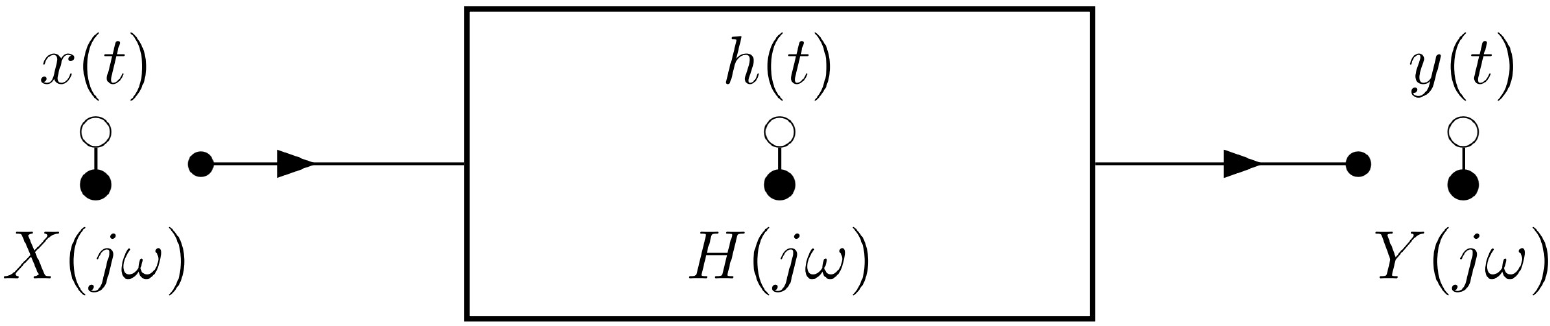
\includegraphics[width=0.7\columnwidth]{images/frequenzgang_impulsantwort.png} \\
\end{center}

Die Impulsantwort $h(t)$ und die Übertragungsfunktion $H(s)$ sind ein\\\
\textbf{Laplace-Transformationspaar}:
$$ \boxed{ h(t) \, \laplace \, H(s) } $$

Das Ausgangssignal berechnet sich als: 
$$ \boxed{ y(t) = h(t) * x(t) \, \laplace \, Y(s) = H(s) \cdot X(s) } $$


\subsubsection{Zusammenhang Impulsantwort - Einheitssprungantwort}

\begin{tabular}{ll}
    $h(t)$ & Impulsantwort \\
    $g(t)$ & Einheitssprungantwort
\end{tabular}

$$ \boxed{ h(t) =  \frac{dg(t)}{dt}  \quad \Leftrightarrow \quad g(t) = \int\limits_{-\infty}^t  h(\tau) \, d \tau }  $$
$$ \boxed{ H(s) = s \cdot G(s) \quad \Leftrightarrow \quad G(s) =  \frac{1}{s} H(s) }  $$


\subsubsection{Zusammenhang Impulsantwort \& Kausalität LTI-System}

\fbox{\parbox{0.9\linewidth}{
Damit ein LTI-System kausal ist, muss dessen Impulsantwort $h(t)$ für alle $t < 0$ gleich Null sein. 
} }

% \texorpdfstring{$\tau_P(\omega)$}{PDFstring} ??
\subsection{Phasenlaufzeit $\tau_P(\omega)$}{183}
Die Phasenlaufzeit ist nur für \textbf{reine Sinus-Schwingungen} exakt bestimmbar! \\
Das System ist beschrieben durch:

$$ x(t) = A \cdot \sin(\omega_0 t + \gamma) $$
$$ H( j \omega) = \alpha \cdot e^{- j \omega t_0} \, \laplace \, h(t) = \alpha \cdot \delta(t - t_0) $$


Das Ausgangssignal $y(t) = x(t) * h(t)$ ist gegenüber dem Eingangssignal $x(t)$ mit Faktor $\alpha$ gewichtet und 
um die Zeit $t_0$ verzögert. \\
$\Rightarrow$ \textbf{Diese Verzögerung wird Phasenlaufzeit genannt}
$$ \boxed{ \tau_P(\omega) = \frac{- \theta(\omega)}{\omega} } $$

$ \theta(\omega)$ entspricht dem Phasengang des Systems 


\example{Phasenlaufzeit}
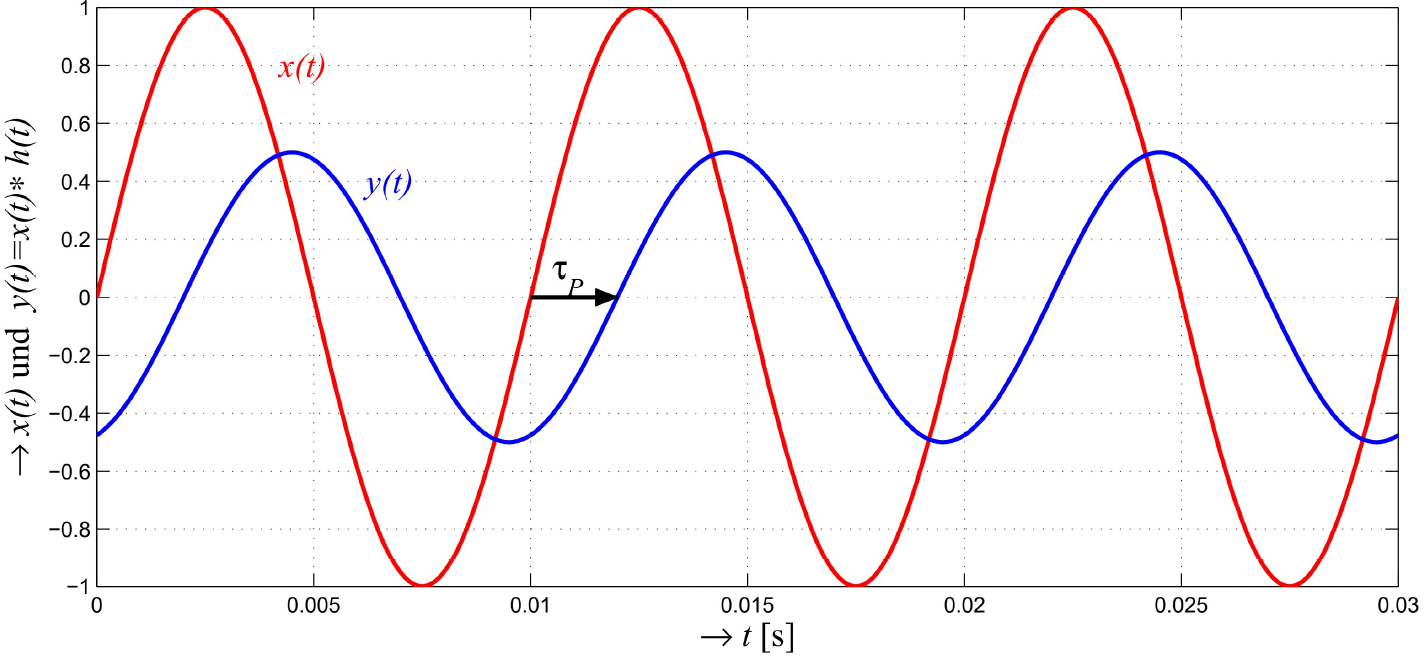
\includegraphics[width=0.8\linewidth]{images/phasenlaufzeit.png}


\subsubsection{Negative Phasenlaufzeit}
Eine negative Phasenlaufzeit bedeutet \textbf{nicht}, dass ein System \textbf{akausal} ist!


\subsection{Gruppenlaufzeit $\tau_G(\omega)$ }{182}
Definiert für Signale mit \textbf{mehreren Frequenzanteilen} \\

Bei amplitudenmodulierten Signalen bestimmt die Gruppenlaufzeit $\tau_G(\omega)$ die \textbf{Verzögerung der Hüllkurve} der AM.

$$ \boxed{ \tau_G(\omega) = \frac{- d \theta(\omega)}{d \omega} } $$

$ \theta(\omega)$ entspricht dem Phasengang des Systems \\

Die Gruppenlaufzeit kann nur dann als \textbf{Laufzeit des Signals} interpretiert werden, wenn im Frequenzbereich des Signales 
die Gruppenlaufzeit und auch die Dämpfung ungefähr konstant sind.


\subsubsection{Negative Gruppenlaufzeit}
Bei \textbf{Vierpolen} mit \textbf{konzentrierten Elementen} ist in bestimmten Frequenzbereichen eine 
\textbf{negative Gruppenlaufzeit} möglich, insbesondere in Frequenzbereichen wo die Dämpfung stark ändert.
(z.B. Nullstellen der UTF) 

Bei negativer Gruppenlaufzeit erscheint die Wirkung \textbf{nicht} vor der Ursache! \\
$\Rightarrow$ Das System ist \textbf{nicht} akausal! \\
Das Maximum der Hüllkurve am Ausgang kann aber \textbf{früher} als am Eingang auftreten.


\subsection{Phasenlaufzeit / Gruppenlaufzeit identisch}{186}
\label{Phasenlaufzeit / Gruppenlaufzeit identisch}
Die \textbf{Signalverzögernug, Phasenlaufzeit} $\tau_P(\omega)$ und \textbf{Gruppenlaufzeit} 
$\tau_G(\omega)$ sind identisch, wenn
$$ \boxed{ \theta(\omega) = - \omega \cdot t_0  } $$

und der \textbf{Amplitudengang ebenfalls konstant} ist, d.h. $H(j \omega) = \alpha \cdot e^{-j \omega t_0}$ \\
Die Signalverzögerung beträgt für \textbf{alle Frequenzen} $t_0 \, (= \tau_P = \tau_G) $ 


\subsection{Verzerrungen}{187-188}

Stimmt der zeitliche Verlauf einer Schwingung auf der Empfängerseite nicht mehr mit der Senderseite überein, arbeitet das
Übertragungssystem \textbf{nicht verzerrungsfrei}.


\subsubsection{Lineare Verzerrung}
Eine \textbf{Dämpfung} eines Signals (z.B. durch einen Tiefpassfilter) entspricht einer \textbf{linearen Verzerrung}


\subsubsection{Nichtlineare Verzerrung}
Nichtlineare Verzerrungen werden durch \textbf{Übersteuerung} des Systems \textbf{(Kanal)} oder dessen
\textbf{nichtlineare Kennlinie} hervorgerufen werden. \\
Durch nichtlineare Verzerrungen treten \textbf{neue}, im Ursprungssignal nicht enthaltene \textbf{Schwingungen} auf.\\
Ein \textbf{Mass} für nichtlineare Verzerrungen ist der \textbf{Klirrfaktor}


\subsection{Klirrfaktor}{189}

Verhältnis des \textbf{Effektivwerts} der \textbf{neu} am Ausgang eines Systems entstandenen \textbf{Harmonischen} zum 
Effektivwert des gesamten Signals

\begin{minipage}[c]{0.48\columnwidth}
    $$ \boxed{ k = \sqrt{\frac{U_2^2 + U_3^2 + ...+ U_n^2}{U_1^2 + U_2^2 + ...+ U_n^2}}} $$
\end{minipage}
\hfill
\begin{minipage}[c]{0.48\columnwidth}
    $U_1$ entspricht der Grundharmonischen
    \textrightarrow Es gilt: $1 > k \geq 0$
\end{minipage}


\subsubsection{Klirrdämpfungsmass}
$$ \boxed{ a_k = 20 \cdot \log_{10} \Big( \frac{1}{k}  \Big)  } $$


\subsubsection{Total Harmonic Disortion (THD)}
Wird vor allem im englisch-sprachigen Raum verwendet

\begin{minipage}[c]{0.48\columnwidth}
   $$ \boxed{  \text{THD} = \sqrt{\frac{U_2^2 + U_3^2 + ...+ U_n^2}{U_1^2} } } $$
\end{minipage}
\hfill
\begin{minipage}[c]{0.48\columnwidth}
    $U_1$ entspricht der Grundharmonischen 
    \textrightarrow Es gilt:  $\infty > \text{THD} \geq 0$ 
\end{minipage}

\vspace{0.2cm}
geringe Verzerrungen: $\text{THD} \approx k$ \qquad allgemein: $\text{THD} > k$


\subsection{Verzerrungsfreie Übertragung von Signalen}{190}
Frequenzgang $H(j \omega)$ und Impulsantowort $h(t)$ eines verzerrungsfreien Signals:

$$ \boxed{ H(j \omega) = \alpha \cdot e^{- j \omega t_0} = | H(j \omega)|  \cdot e^{j \theta(\omega)}  \, \laplace \,  h(t) = \alpha \cdot \delta(t - t_0) } $$


Damit ein Signal verzerrungsfrei übertragen wird, müssen folgende Bedingungen erfüllt sein:

\begin{enumerate}
    \item \textbf{Amplitude} konstant (unabhängig von der Frequenz) $\Leftrightarrow | H(j \omega)| = \text{konstant} = \alpha \neq 0$ 
        \textrightarrow Keine Amplitudenverzerrung vorhanden
    \item \textbf{Phase} proportional zur Frequenz $\Leftrightarrow \theta(\omega) = - \omega \, t_0$
        (äquivalenz zu Abschnitt \ref{Phasenlaufzeit / Gruppenlaufzeit identisch})
        \textrightarrow Keine Phasenverzerrung vorhanden
\end{enumerate}


\subsection{Übertragung stochastischer Signale}{193-194}
Wird ein stochastisches Signal $x(t)$ (schwach stationär) durch ein LTI-System mit Impulsantowort $h(t)$ übertragen, so berechnet
sich das Ausgangssignal $y(t)$ gemäss Abschnitt \ref{Zusammenhang} aus

$$ \boxed{ y(t) = h(t) * x(t) = \int\limits_{- \infty}^{\infty} x(\tau) \, h(t - \tau) \, \diff \tau  \, 
\laplace \, Y(s) = H(s) \cdot X(s) } $$


\subsubsection{Linearer Mittelwert}
Der lineare Mittelwert $Y_0$ des Ausgangssignals $y(t)$ bei der Frequenz $\omega = 0$ entspricht

$$ \boxed{ Y(j0) = X(j0) \cdot H(j0) \Rightarrow Y_0 = X_0 \cdot H(j0) } $$

$H(j \omega)$ = Frequenzgang und $X_0$ = linearer Mittelwert von $x(t)$ 


\subsubsection{Autokorrelationsfunktion (AKF) des Ausgangssignals}
Da $\varphi_{yy}(\tau)$ und $Y_0$ nicht von $t$ abhängen, ist auch $y(t)$ schwach stationär.

$$ \boxed{ \varphi_{yy}(\tau) = \int\limits_{- \infty}^{\infty} \int\limits_{- \infty}^{\infty} h(\alpha) \, h(\beta) \, \varphi_{xx}(\tau + \alpha - \beta) \, \diff \alpha \, \diff \beta 
= h(-\tau) * h(\tau) * \varphi_{xx}(\tau) } $$

Es gelten folgende Zusammenhänge für die Fourier-Transformationspaare \\

\begin{tabular}{l c l | l c l}
    $h(-\tau)$              & $\laplace$ & $H^*(j \omega)$      & $\varphi_{xx}(\tau)$ & $\laplace$ & $\Phi_{xx}(j \omega)$ \\
    $h(\tau)$               & $\laplace$ & $H(j \omega)$        & $h(\tau) * h(-\tau)$ & $\laplace$ & $|H(j \omega)|^2$
\end{tabular}


\subsubsection{Leistungsdichtespektrum (PSD)}
Die AKF und das PSD sind ein Fourier-Transformationspaar
$$ \underbrace{\varphi_{yy}(\tau)}_{\text{AKF}} \, \laplace \, \underbrace{\Phi_{yy}(j \omega)}_{\text{PSD}} $$

Daraus folgt der Zusammenhang der Leistungsdichtespektren $\Phi(j \omega)$
$$ \boxed{ \Phi_{yy}(j \omega) = |H(j \omega)|^2 \, \Phi_{xx}(j \omega) } $$

Für die AKF des Ausgangssignals $y(t)$ gilt 
$$ \boxed{ \varphi_{yy}(\tau) = \frac{1}{2 \pi} \int\limits_{- \infty}^{\infty} |H(j \omega)|^2 \, \Phi_{xx}(j \omega) \, e^{j \omega \tau} \diff \omega } $$

Die Leistung $Y^2$ des Ausgangssignals $y(t)$ berechnet sich beim Zeitpunkt $\tau = 0$ als
$$ \boxed{ Y^2 = \varphi_{yy}(0) = \frac{1}{2 \pi} \int\limits_{- \infty}^{\infty} |H(j \omega)|^2 \, \Phi_{xx}(j \omega) \, \diff \omega } $$


\subsubsection{Kreuzkorrelationen}
Die Kreuzkorrelationsfunktionen $\varphi_{xy}(\tau)$ und $\varphi_{yx}(\tau)$ des stochastischen, reellen Eingangssignals $x(t)$ 
(Klasse 2b) und des stochastischen Ausgangssignals $y(t)$ eines LTI-Systems hängen folgendermassen zusammen:

$$ \boxed{ \varphi_{xy}(\tau) = h(\tau) * \varphi_{xx}(\tau) \, \laplace \, \Phi_{xy}(j \omega) = H(j \omega) \cdot \Phi_{xx}(j \omega) } $$
$$ \boxed{ \varphi_{yx}(\tau) = h(-\tau) * \varphi_{xx}(\tau) \, \laplace \, \Phi_{yx}(j \omega) = H^*(j \omega) \cdot \Phi_{xx}(j \omega) } $$

Somit gilt:
$$ \boxed{ \varphi_{yx}(\tau) = \varphi_{xy}(-\tau) \, \laplace \, \Phi_{yx}(j \omega) = \Phi_{xy}(-j \omega) = \Phi^*_{xy}(j \omega) } $$
        \section{Dämpfung, Verstärkung, Dezibel}

Hinweis: Neben Dezibel gibt es ein weiteres Dämpfungs-/ bzw. Verstärkungsmass: Neper $\neper$
Auf dieses Mass wird allerdings nicht genauer eingegangen. Skript: S.207


\subsection{Dämpfungsfaktor \texorpdfstring{$D$}{D}}{206}

Das Verhältnis zwischen Eingangs- und Ausgangssignal wird als Dämpfungsfaktor $D$ bezeichnet

\begin{minipage}[c]{0.3\columnwidth}
    $$ \boxed{ D_{P} = \frac{P_{1}}{P_{2}} } $$
\end{minipage}
\hfill
\begin{minipage}[c]{0.3\columnwidth}
    $$ \boxed{ D_{U} = \frac{U_{1}}{U_{2}} } $$
\end{minipage}
\hfill
\begin{minipage}[c]{0.3\columnwidth}
    $$ \boxed{ D_{I} = \frac{I_{1}}{I_{2}} } $$
\end{minipage}

Die Indizes $U$, $P$, $I$ stehen für die \textbf{Effektivwerte} von Spannung, Leistung und Strom.


\subsection{Dämpfungsmass \texorpdfstring{$a$}{a} in Dezibel}{206}

Durch \textbf{logarithmieren} des Dämpfungsfaktors $D$ erhält man das Dämpfungsmass $a$

\begin{minipage}[c]{0.3\columnwidth}
    $$ \boxed{ a_{P} =  10 \cdot \log_{10} \Big( \frac{P_{1}}{P_{2}} \Big) } $$
\end{minipage}
\hfill
\begin{minipage}[c]{0.3\columnwidth}
    $$ \boxed{ a_{U} = 20 \cdot \log_{10} \Big( \frac{U_{1}}{U_{2}} \Big) } $$
\end{minipage}
\hfill
\begin{minipage}[c]{0.3\columnwidth}
    $$ \boxed{ a_{I} = 20 \cdot \log_{10} \Big( \frac{I_{1}}{I_{2}} \Big) } $$
\end{minipage}


\subsubsection{Umrechnung Verstärkungsfaktor -- Dezibel}

$$ \boxed{ \deci\bel = 10 \cdot \log_{10} (v) \, \Leftrightarrow \, v = 10^{\frac{\deci\bel}{10}} } $$


\subsection{Rechenregeln mit Dezibel}

\begin{itemize}
    \item Faktoren multiplizieren \textrightarrow\ Dezibel-Werte addieren
    \item Faktoren dividieren \textrightarrow\ Dezibel-Werte subtrahieren
\end{itemize}


\subsection{Spannungsverstärkungsfaktor}{209}

Hält man sich strikt an die Definition des Verstärkungsfaktors bzw. die Definition der Dezibel, so würde man für Dämpfungen positive
Dezibel-Werte erhalten und für Verstärkungen entspreched negative Dezibel-Werte. Dies ist gegen die Intuition des Ingenieurs. \\
Somit wurde der \textbf{Spannungsverstärkungsfaktor} $\bm{T_{U}}$ definiert. Analog zum Dämpfungsmass $a$ wird ein 
\textbf{Verstärkungsmass} $\bm{g_{U}}$ definiert.

\begin{minipage}[c]{0.48\columnwidth}
    $$ \boxed{ T_U = \frac{U_2}{U_1} } $$
\end{minipage}
\hfill
\begin{minipage}[c]{0.48\columnwidth}
    $$ \boxed{ g_U = 20 \cdot \log_{10} \Big( \frac{U_2}{U_1} \Big) } $$
\end{minipage}


Aus dieser Definition folgt für die Dezibel-Werte:

\begin{itemize}
    \item \textbf{Verstärkung: } ($U_2 > U_1$) \textrightarrow\ positive Dezibel-Zahl
    \item \textbf{Dämpfung: } ($U_2 < U_1$) \textrightarrow\ negative Dezibel-Zahl
\end{itemize}


\example{Kaskadiertes System}{209}

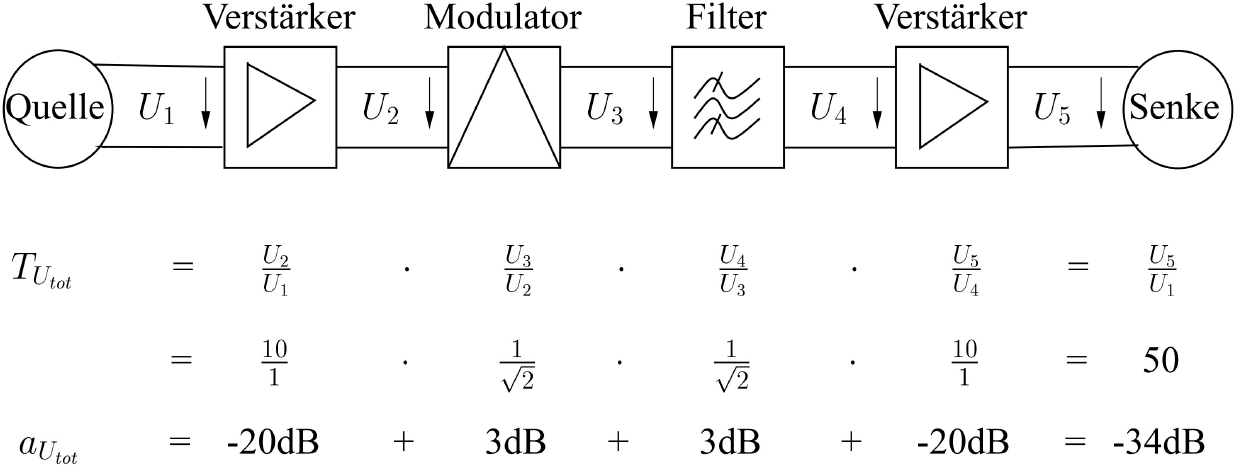
\includegraphics[width=0.9\columnwidth]{images/kaskadierung_verstaerkung_daempfung.png}

Formuliert mit dem Verstärkungsmass $g$ ergeben sich umgekehrte Vorzeichen:
$$ g_{U_{tot}} \quad = \quad - 20 \, \deci\bel \quad  + \quad 3 \, \deci\bel \quad + 
    \quad 3 \, \deci\bel \quad - \quad 20 \, \deci\bel \quad = \quad -34 \, \deci\bel $$



\subsection{Umrechnungs-Tabelle Dezibel -- Faktor}

\textbf{Vorgehen:} Gesuchten $\deci\bel$-Wert als Summe / Differenz von bekannten Werten darstellen\\
\textrightarrow\ Summanden in Faktoren 'transferieren' und multiplizieren / dividieren \medskip

\textbf{Vorgehen:} Gesuchten Faktor als Produkt / Quotent von bekannten Werten darstellen\\
\textrightarrow\ Faktoren in Summanden 'transferieren' und addieren / subtrahieren \medskip


\begin{ctabular}{l l}
    \toprule
    \textbf{Dezibel}        & \textbf{Faktor} \\
    \midrule
    $20 = 10 + 10$          & $100 = 10 \cdot 10$ \\ 
    $12$                    & $16 = 2 \cdot 2 \cdot 2 \cdot 2$ \\
    $\cor{10}$              & $\cor{10}$ \\
    $9 = 3 + 3 + 3$         & $8 = 2 \cdot 2 \cdot 2$ \\
    $8 = 5 - 3$             & $6.4 = 3.2 \cdot 2$ \\
    $7 = 10 -3$             & $5 = \frac{10}{2}$ \\
    $6 = 3 + 3$             & $4 = 2 \cdot 2$ \\
    $5 = 15 - 10$           & $3.2 = \frac{32}{10\mathstrut} \approx \sqrt{10}$ \\
    $4 = 10 - 6 = 10 - 3-3$ & $2.5 = \frac{10\mathstrut}{2 \cdot 2}$ \\
    $\cor{3}$               & $\cor{2}$ \\
    $2= 12-10= 5-3$         & $1.6 = \frac{16}{10}$ \\
    $1 = 10 - 3 - 3 - 3$    & $1.25 = \frac{10}{2\cdot 2 \cdot 2} = \frac{5}{4}$ \\
    $\cor{0}$               & $\cor{1}$ \\
    $-1$                    & $0.8 = \frac{4}{5}$ \\
    \bottomrule
\end{ctabular}


\subsection{Relativer und Absoluter Pegel}{210}

Bei den bisher ausgeführten Pegeln handelt es sich um \textbf{relative Pegel}. Im Gegensatz dazu beziehen sich
\textbf{absolute Pegelangaben} immer auf eine Referenzgrösser (erzeugt von einem Normengenerator, siehe Skript). 

\renewcommand{\arraystretch}{1.7}
\begin{tabular}{c c c}
    ${(L_{U})}_{\text{rel}} = 20 \cdot \log_{10} \left\lgroup \frac{U_2}{U_1} \right\rgroup$ & &
    ${(L_{U})}_{\text{abs}} = 20 \cdot \log_{10} \left\lgroup \frac{U_2}{774.6 \, \milli\volt} \right\rgroup$ \\
    
    ${(L_{I})}_{\text{rel}} = 20 \cdot \log_{10} \left\lgroup \frac{I_2}{I_1} \right\rgroup$ & &
    ${(L_{I})}_{\text{abs}} = 20 \cdot \log_{10} \left\lgroup \frac{I_2}{1.291 \, \milli\ampere} \right\rgroup$ \\
    
    ${(L_{P})}_{\text{rel}} = 10 \cdot \log_{10} \left\lgroup \frac{P_2}{P_1} \right\rgroup$ & &
    ${(L_{P})}_{\text{abs}} = 10 \cdot \log_{10} \left\lgroup \frac{P_2}{1 \, \milli\watt} \right\rgroup$ \\
\end{tabular}
\renewcommand{\arraystretch}{1}


\subsubsection{Kennzeichnung absoluter Pegel}

\begin{center}
    \begin{tabular}{ll}
        \textbf{Notation}       & \textbf{Bezugsgrösse} \\
        $\deci\bel\watt$        & $1 \, \watt$          \\
        $\deci\bel\volt$        & $1 \, \volt$          \\
    \end{tabular}\hspace{5mm}
    \begin{tabular}{ll}
        \textbf{Notation}       & \textbf{Bezugsgrösse} \\
        $\deci\bel\milli$       & $1 \, \milli \watt$ \\
        $\deci\bel\micro\volt$  & $1 \, \micro \watt$ 
    \end{tabular}
\end{center}

        \section{Frequnzverhalten analoger LTI-Systeme}

\begin{minipage}[c]{0.5\columnwidth}
    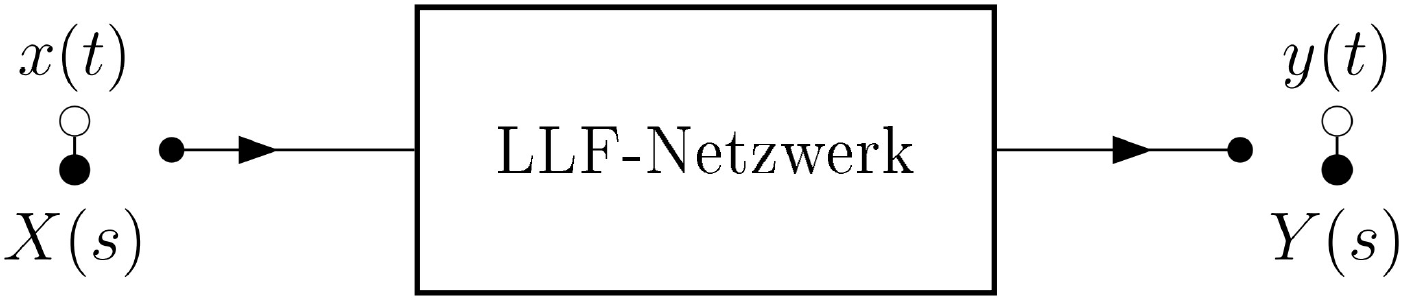
\includegraphics[width=\columnwidth]{images/llf_netzwerk.png}
\end{minipage}
\hfill
\begin{minipage}[c]{0.48\columnwidth}
    \raggedright% needed to suppress underfull hbox warning
    Die Betrachtungen beschränken sich auf \textbf{zeitinvariante} LLF-Netzwerke (lineare Netzwerke mit konzentrierten Elementen)
\end{minipage}




\subsection{Zusammenhang Frequenzgang -- UTF}{211}

Alle LTI-Systeme lassen sich mit einer Differntialfleichung der folgenden Form beschreiben:
$$ a_n \frac{\diff^n y}{\diff t^n} + a_{n-1} \frac{\diff^{n-1} y}{\diff t^{n-1}} + \cdots + a_1 \frac{\diff y}{\diff t} + a_0 y =
    b_m \frac{\diff^m x}{\diff t^m} + b_{m-1} \frac{\diff^{m-1} x}{\diff t^{m-1}} + \cdots + b_1 \frac{\diff x}{\diff t} + b_0 x  $$

Die Laplace-Transformierte der DGL hat die Form 
$$ \boxed{ H(s) = \frac{Y(s)}{X(s)} = \frac{b_m s^m + b_{m-1} s^{m-1} + \cdots + b_1 s + b_0}
{a_n s^n + a_{n-1} s^{n-1} + \cdots + a_1 s + a_0}  = \frac{N(s)}{D(s)} }$$

\begin{ctabular}{Ol}
    N(s) & Zählerpolynom mit konstanten, reelen Koeffizienten \\
    D(s) & Nennerpolynom mit konstanten, reelen Koeffizienten \\
    x(t) & Eingangssignal \\
    y(t) & Ausgangssignal \\
\end{ctabular}

\vspace{0.2cm}

Die Wurzeln der Gleichung $N(s) = 0$ ergeben $m$ endliche Nullstellen; die Wurzeln von $D(s) = 0$ ergeben $n$ Pole des Systems.
\textbf{Aus Stabilitätsgründen müssen alle Pole in der linken Halbebene (LHE) liegen!}


\subsubsection{Praktische Schreibweise für Pol-/Nullstellen}

Um die Pole bzw. Nullstellen des Systems direkt ablesen zu können, wird $H(s)$ faktorisiert. \textrightarrow\ Die UTF $H(s)$ ist durch
die Pole, Nullstellen und den Faktor K \textbf{vollständig bestimmt}!

$$ H(s) = \underbrace{\frac{b_m}{a_m}}_{K} \cdot \frac{\prod\limits_{i=1}^m (s - z_i)}{\prod\limits_{j=1}^n (s - p_j)} $$


Da die Wurzeln von Polynomen mit reellen Koeffizienten entweder reell oder konjugiert-komplexe Paare auftreten, ist es meistens
sinnvoll, die Systemfunktionen als Produkt von Faktoren 1. und 2. Ordnung mit reelen Koeffizienten darzustellen.

$$ H(s) = \underbrace{\frac{b_m}{a_m}}_{K} \cdot 
    \frac{\prod\limits_{i=1}^r (\cbl{s^2 + 2 \sigma_{zi} s + \omega_{zi}^2}) \prod\limits_{i=2r+1}^m (\cgn{s - z_i})}
    {\prod\limits_{j=1}^t (\cor{s^2 + 2 \sigma_{pj} s + \omega_{pj}^2}) \prod\limits_{j=2t+1}^n (\cvt{s - p_j})} $$

\textbf{Legende:}
\begin{itemize}
    \item \cbl{Beschreibt komplex-konjugierte Nullstellen in der LHE} 
    \item \cgn{Beschreibt reelle Nullstellen in der LHE}
    \item \cor{Beschreibt komplex-konjugierte Polein der LHE} 
    \item \cvt{Beschreibt reelle Pole in der LHE} 
\end{itemize}

\vspace{0.2cm}

Alternativ kann $H(s)$ mittels \textbf{Polfrequenzen} und \textbf{Polgüten} beschrieben werden:
$$ H(s) = \underbrace{\frac{b_m}{a_m}}_{K} \cdot 
    \frac{\prod\limits_{i=1}^r (s^2 + \frac{\omega_{zi}}{q_{zi}} s + \omega_{zi}^2) \prod\limits_{i=2r+1}^m (s - z_i)}
    {\prod\limits_{j=1}^t (s^2 +\frac{\omega_{pj}}{q_{pj}} s + \omega_{pj}^2) \prod\limits_{j=2t+1}^n (s - p_j)} $$

\begin{ctabular}{Ol Ol}
    \omega_{pj}   & Polstellenfrequenzen  & \omega_{zi}   & Nullstellenfrequenzen \\
    q_{pj}        & Polstellengüten       & q_{zi}        & Nullstellengüten
\end{ctabular}


\subsection{Pol- und Nullstellendiagramme}{212}

\begin{minipage}[c]{0.35\columnwidth}
    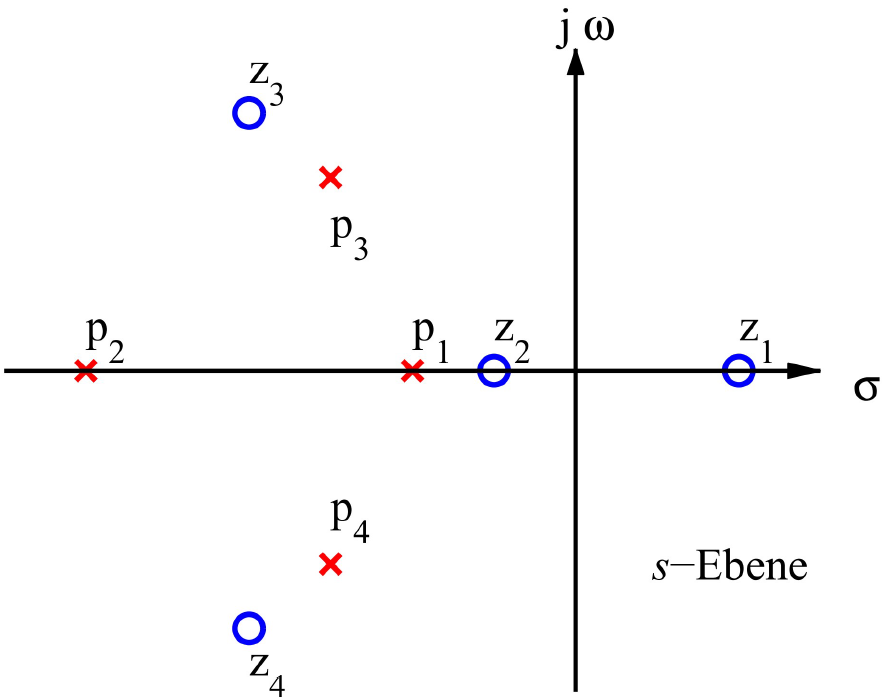
\includegraphics[width=\columnwidth]{images/pol_nullstellen_diagramm.png}
\end{minipage}
\hfill
\begin{minipage}[c]{0.63\columnwidth}
    Werden die Pole und Nullstellen in der komplexen Zahlenebene dargestellt, so spricht man von einem Pol-/Nullstellen-Diagramm.

    In Matlab erzeugt der Befehl \texttt{pzmap} einen solchen Plot

    \begin{tabular}{ll}
        Pole    & Kreuze \\
        NS      & Kreise \\
    \end{tabular}
\end{minipage}


\subsection{Pole in der komplexen Zahlenebene}{214}

\example{Polynom 2. Ordnung mit komplex-konjugierten Polen}

\begin{minipage}[c]{0.45\columnwidth}
    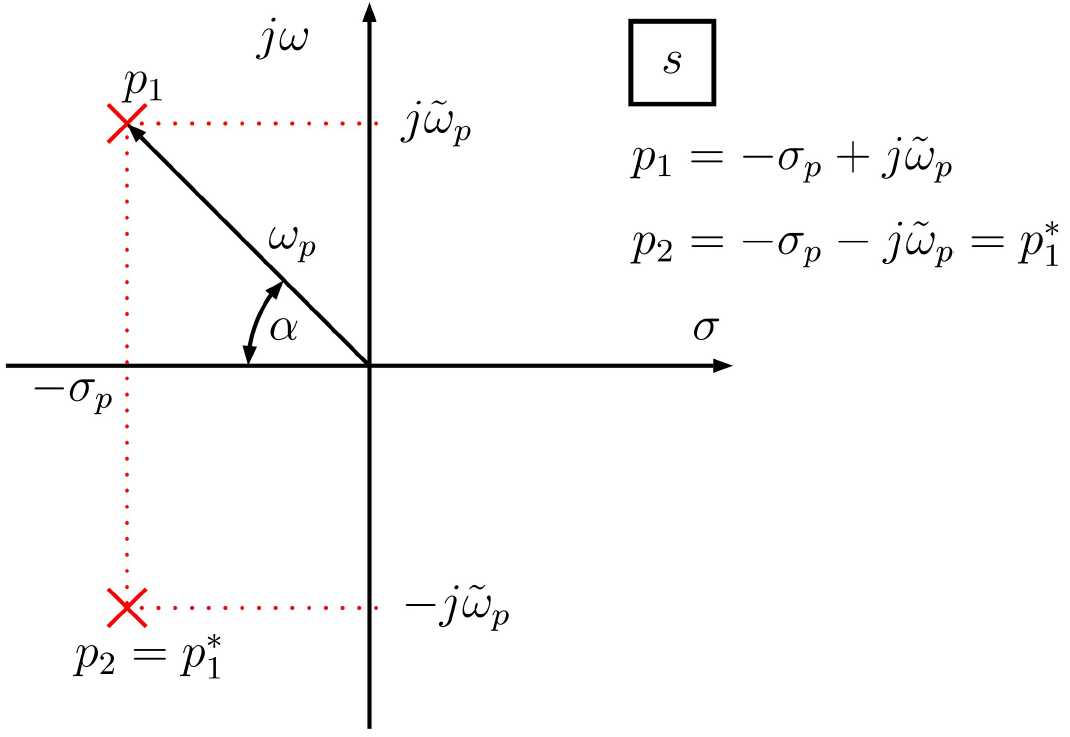
\includegraphics[width=\columnwidth]{images/beispiel_pol_nullstellen_diagramm.png}
\end{minipage}
\hfill
\begin{minipage}[c]{0.48\columnwidth}
    $$(s - p_1) \cdot (s -p_2) = s^2 + 2 \sigma_p s + (\sigma_p^2 + \tilde{\omega}_p^2) $$
    $$ \boxed{ \omega_p = \sqrt{\sigma_p^2 + \tilde{\omega}_p^2}} $$
    $$ \boxed{ q_p = \frac{\omega_p}{2 \sigma_p} = \frac{1}{2 \cdot \cos(\alpha)}} $$
\end{minipage}

\begin{tabular}{ll}
    $\omega_p$  & Polfrequenz \textrightarrow\ Entspricht Abstand des Pols vom Ursprung \\
    $q_p$       & Polgüte \\
\end{tabular}

\vspace{0.2cm}
\textbf{\myul{Grenzfälle}} \\
\begin{tabular}{lll}
    $\sigma_p = \omega_p$   & Doppelpol auf neg. reeller Achse  & \textrightarrow\ $q_p = \frac{1}{2}$ \\
    $\sigma_p = 0$          & Polpar auf imaginärer Achse       & \textrightarrow\ $q_p = \infty$
\end{tabular}


\subsubsection{Reelle Pole}

\begin{minipage}[c]{0.48\columnwidth}
    $$ \boxed{ \omega_p = \sqrt{\sigma_{p1} \cdot \sigma_{p2} } } $$
\end{minipage}
\hfill
\begin{minipage}[c]{0.48\columnwidth}
    $$ \boxed{ q_p =  \frac{\sqrt{\sigma_{p1} \cdot \sigma_{p2}}}{\sigma_{p1} + \sigma_{p2}} \leq \frac{1}{2} } $$
\end{minipage}

\begin{itemize}
    \item[\textrightarrow] Für einzelne (reelle) Pole ist ist die Güte $q_p$ nicht definiert.
    \item[\textrightarrow] Die Polfrequenz $\omega_p$ entspricht dem Abstand zum Ursprung.
\end{itemize}

\textbf{\myul{Identische Werte}} \\
\begin{tabular}{c c c}
    $\sigma_{p1} = \sigma_{p2}$ & & $| q_p | = \frac{1}{2}$
\end{tabular}


\subsubsection{Verallgemeinerung des Beispiels}{214}

\begin{minipage}[c]{0.55\columnwidth}
    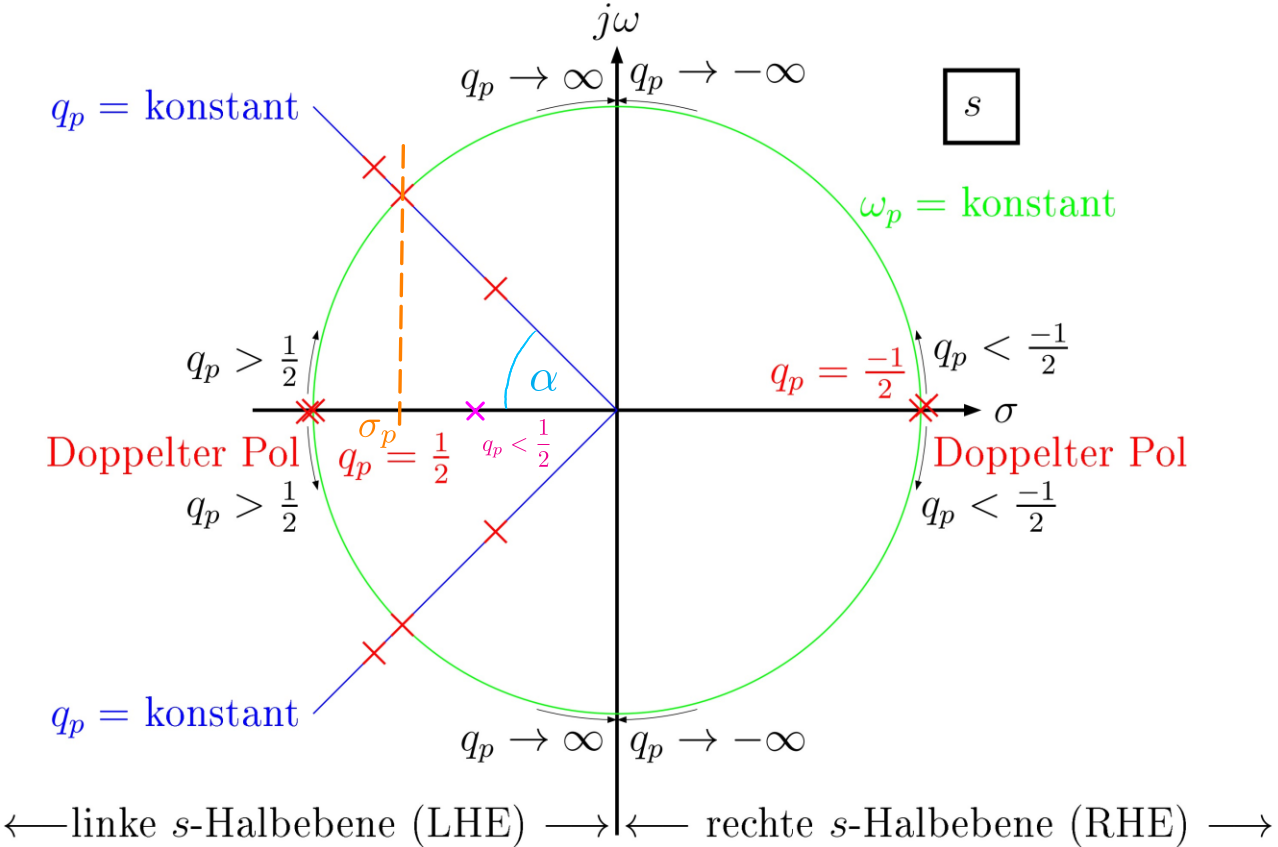
\includegraphics[width=\columnwidth]{images/pole_nullstellen_koeffizienten.png}
\end{minipage}
\hfill
\begin{minipage}[c]{0.42\columnwidth}
    \raggedright% needed to suppress underfull hbox warning
    \textbf{Hinweise}
    \begin{itemize}
        \item Pole sind als rote Kreuze dargestellt
        \item Für die NS (Nullstellenfrequenzen, Nullstellengüten) gelten die gleichen
            geometrischen Beziehungen wie für die Polstellen
    \end{itemize}
\end{minipage}




\subsection{Bestimmung Frequenzgang aus UTF}{216}

Um den Frequenzgang zu erhalten, kann $s = j \omega$ eingesetzt werden.

$$ \boxed{ H(j \omega) = H(s) \Big|_{s = j \omega} = |H(j \omega)| \cdot e^{j \theta(\omega)} } $$

\begin{center}
    \begin{tabular}{ll}
        $H(s)$              & Übertragungsfunktion (UTF) \\
        $H(j \omega)$       & Frequenzgang 
    \end{tabular}\hspace{5mm}
    \begin{tabular}{ll}
        $|H(j \omega)|$     & Amplitudengang \\
        $\theta(\omega)$    & Phasengang
    \end{tabular}
\end{center}

Der Frequenzgang bzw. Amplitudengang und Phasengang werden folgendermassen dargestellt:

\begin{itemize}
    \item Nyquist-Diagramm \\
        $H(j \omega)$ wird in Polarkoordinaten mit $\omega$ als Parameter aufgezeichnet 
    \item \textbf{Bode-Diagramm} \\
        $\alpha_{\deci \bel}(\omega)$ und $\theta(\omega)$ werden je in Funktion von $\log_{10}(\omega)$ aufgezeichnet
\end{itemize}


\subsection{Bestimmung Frequenzgang aus Pol- / Nullstellendiagramm}

Durch einsetzen einer beliebigen Auswertungsfrequenz $j \omega_0$ in die Übertragungsfunktion $H(s)$ ergibt sich der
Frequenzgang $H(j \omega_0)$ als:

$$ H(j \omega_0) = K \cdot \frac{(j \omega_0 - z_1) (j \omega_0 - z_2) \cdots (j \omega_0 - z_m)}
                                {(j \omega_0 - p_1) (j \omega_0 - p_2) \cdots (j \omega_0 - p_n)}
                                = | H(j \omega_0) | \cdot e^{j \theta (\omega_0)} $$

Die einzelnen Faktoren in Zähler und Nenner können in Betrag und Phase aufgeteilt werden, beispielsweise folgendermassen:
$$ (j \omega_0 - p_1) = |j \omega_0 - z_1| \cdot e^{j \theta_{z1}} = A_{z1} \cdot e^{j \theta_{z1}} $$



Angewendet auf alle Faktoren kann der Frequenzgang $H(j \omega_0)$ in den \cor{Amplitudengang $|H(j \omega)|$} und den
\cgn{Phasengang $\theta(\omega)$} separiert werden:

$$ \boxed{ H(j \omega_0) = K \cdot \frac{\cor{A_{z1} \cdot A_{z2} \cdots A_{zm}} \cdot \cgn{e^{j(\theta_{z1} + \cdots + \theta_{zm})}}}
                                        {\cor{A_{p1} \cdot A_{p2} \cdots A_{pm}} \cdot \cgn{e^{j(\theta_{p1} + \cdots + \theta_{pm})}}} } $$

\vspace{0.2cm}
\begin{minipage}[t]{0.48\columnwidth}
    \begin{center}
        \textbf{Betrag}
    \end{center}
    \vspace{-0.2cm}
    $$ \boxed{ | H(j \omega_0) | = K \cdot \frac{\prod_{i=1}^{m} A_{zi}}{\prod_{j=1}^{n} A_{pj}} } $$
\end{minipage}
\hfill
\begin{minipage}[t]{0.48\columnwidth}
    \begin{center}
        \textbf{Phase}
    \end{center}
    \vspace{-0.2cm}
    $$ \boxed{ \theta(\omega_0) = \underbrace{\text{Phase von } K}_{\text{meistens } 0} + \sum_{i=1}^{m} \theta_{zi} - \sum_{j=1}^{m} \theta_{pj} } $$
\end{minipage}


\subsubsection{Zusammenhang mit Pol- / Nullstellendiagramm}

\begin{minipage}[c]{0.5\columnwidth}
    \begin{center}
    \begin{tikzpicture}
        [
            scale = 0.6,
            >=latex,
            ns/.style={circle, draw=blue, fill=white, thick, inner sep=0pt, minimum size=3pt},
            pol/.style={cross out, draw=red, inner sep=0pt, minimum size=3pt} 
        ]
        \begin{axis}
            [
                xmin=-4, xmax=2.5, ymin=-5, ymax=5, axis lines=middle,
                x label style={anchor=west},
                xlabel=$\sigma$,
                y label style={anchor=south},
                ylabel=$j \omega$,
                %grid
            ]
            
            % defines for arch
            \def\arrowRadius{5mm}                                           % radius of the circle that the arrow bends around

            % nodes
            \node[label=left: $j \omega_0$, inner sep = 0pt]       (freq0)     at (0, 1)       {};
            \draw                                                   (-0.05, 1) -- (0.05, 1);

            \node[label=left: $j \omega_1$, inner sep = 0pt]        (freq1)     at (0, 3)       {};
            \draw                                                   (-0.05, 3) -- (0.05, 3);

            \node[ns, label=left: $z_1$]                            (z1)        at (-3, 4)      {};
            \draw                                                   (z1) -- (-2, 4);
            \draw [-latex, green, semithick]                        (-2.5, 4) arc (0:330:\arrowRadius); %(start:end:radius)
            \node[label={[green]right:$\theta_{z1}$}]               (theta1)    at (-2.5, 4.3)    {};

            \node[ns, label=left: $z_2$]                            (z2)        at (-3, -4)     {};
            \draw                                                   (z2) -- (-2, -4);   
            \draw [-latex, green, semithick]                        (-2.5, -4) arc (0:45:\arrowRadius);
            \node[label={[green]right:$\theta_{z2}$}]               (theta2)    at (-2.6, -3.7)   {};

            \node[pol, label=below right: $p_1$]                    (p1)        at (1, 2)      {};
            \draw                                                   (p1) -- (2, 2); 
            \draw [-latex, green, semithick]                        (1.5, 2) arc (0:205:\arrowRadius);
            \node[label={[green]right:$\theta_{p1}$}]               (theta3)    at (1.5, 2.3)    {};

            \node[pol, label=below: $p_2$]                          (p2)        at (1, -2)     {};
            \draw                                                   (p2) -- (2, -2); 
            \draw [-latex, green, semithick]                        (1.5, -2) arc (0:125:\arrowRadius);
            \node[label={[green]right:$\theta_{p2}$}]               (theta4)    at (1.5, -1.7)    {};

            
            \draw[thick, orange]        (freq0) to node[above]      {$A_{z1}$}  (z1);
            \draw[thick, orange]        (freq0) to node[below]      {$A_{z2}$}  (z2);
            \draw[thick, orange]        (freq0) to node[below right]{$A_{p1}$}  (p1);
            \draw[thick, orange]        (freq0) to node[below left] {$A_{p2}$}  (p2);
           
        \end{axis}
        
    \end{tikzpicture}
\end{center}

    % Hier mit nur einer Nullstelle (keine Pole): 
    % 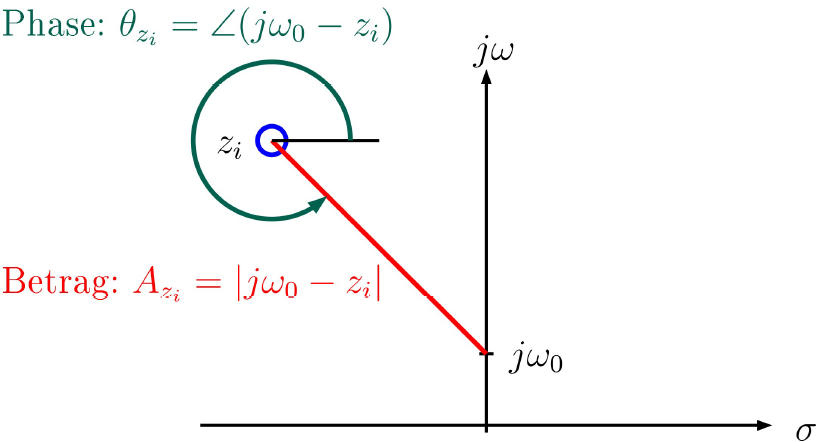
\includegraphics[width=\columnwidth]{images/frequenzgang_amplitudengang.png}
\end{minipage}
\hfill
\begin{minipage}[c]{0.48\columnwidth}
    Die Auswertungsfrequenz $j \omega$ ist variabel und 'wandert' auf der \textbf{imaginären Achse}.
    Für ein bestimmte Auswertungsfrequenz $j \omega_0$ können die Faktoren von $H(j \omega_0)$ als \cor{Abstand}
    und \cgn{Phase} zu den Pol- bzw Nullstellen interpretiert werden.
    Somit kann grafisch aus dem Pol- Nullstellendiagramm ein Rückschluss auf den Amplitudengang gezogen werden.
    $$ H(j \omega_0) = K \cdot \frac{\cor{A_{z1} \cdot A_{z2}} \cdot \cgn{e^{j(\theta_{z1} + \theta_{z2})}}}
    {\cor{A_{p1} \cdot A_{p2}} \cdot \cgn{e^{j(\theta_{p1} + \theta_{p2})}}}  $$
\end{minipage}


\subsubsection{Rückschlüsse auf Amplitudengang}

\begin{outline}
    \1 Es werden vor allem die \textbf{Abstände} betrachtet 
    \1 Pol- und Nullstellen können sich aufheben
    \1 Bei $\omega = 0$ gilt:
        \2 Wenn Nullstelle \textrightarrow\ $|H(j \omega_0)| = \infty$ \textrightarrow\ $\theta(j \omega_0) = \frac{\pi}{2}$
        \2 Wenn Pol \textrightarrow\ $|H(j \omega_0)| = 0$ \textrightarrow\ $\theta(j \omega_0) = -\frac{\pi}{2}$
        \2 Wenn weder Pol noch NS \textrightarrow\ $|H(j \omega_0)|$ hat endlichen Wert \textrightarrow\ $\theta(j \omega_0) = 0$
    \1 Bei $\omega = \infty$ gilt:
        \2 Wenn Zählergrad $>$ Nennergrad \textrightarrow\ $|H(j \omega_0)| = \infty$
        \2 Wenn Zählergrad $=$ Nennergrad \textrightarrow\ $|H(j \omega_0)|$ hat endlichen Wert
        \2 Wenn Zählergrad $<$ Nennergrad \textrightarrow\ $|H(j \omega_0)| = 0$
\end{outline}


\subsection{Allpass(netzwerk)}{220}

Ein Allpass ist ein Netzwerk, bei dem der \textbf{Amplitudengang für alle Kreisfrequenzen $\bm{\omega}$ konstant} ist
$$ \boxed{\abs{H(\jimg \omega)} = \text{ konst } \neq 0}$$

\textrightarrow\ Im Pol-Nullstellen-Diagramm ist ein Allpass dargestellt durch eine 
\textbf{zur $\bm{\jimg \omega}$-Achse symmetrische Pol-Nullstellenkonfiguration}

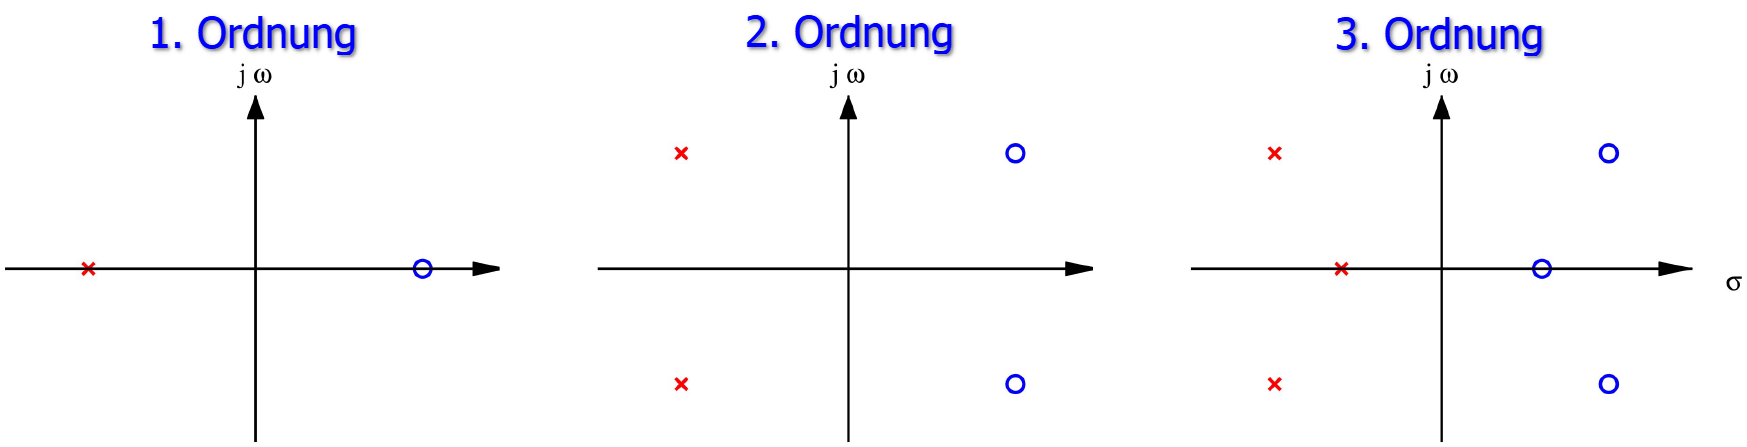
\includegraphics[width=\columnwidth]{images/allpass.png}

$$ \boxed{ \text{UTF Allpass: } H_A(s) = K \cdot \frac{Q(-s)}{Q(s)} } $$

Für einen Allpass gilt:
\begin{itemize}
    \item Ein stabiler Allpass besitzt einen \textbf{streng monoton abfallenden} Phasengang
    \item Jede beliebige (realisierbare) UTF $H(S)$ kann \textbf{immer} in ein allpassfreies Netzwerk $H_M(s)$ und einen Allpass $H_A(s)$
        \textbf{zerlegt} werden (\textrightarrow\ siehe Beispiel Abschnitt ~\ref{Beispiel Zerlegung})
        $$ \boxed{ H(s) = H_M(s) \cdot H_A(s) }$$
\end{itemize}


\subsection{Minimalphasige- und nicht-minimalphasige Systeme}{221}

\begin{outline}
    \1 Minimalphasennetzwerke: 
        \2 besitzen \textbf{keine Nullstellen in der rechten Halbebene (RHE)}
        \2 \textbf{entweder} ein frei wählbarer Amplituden- \textbf{oder} Phasengang
    \1 Nicht-Minimalphasennetzwerke
        \2 Amplituden- und Phasengang unabhängig voneinander wählbar
\end{outline}


\example{Zerlegung nicht-minimalphasiges System}
\label{Beispiel Zerlegung}

Ein nicht-minimalphasiges System kann in ein minimalphasiges System und einen Allpass zerlegt werden
(\textrightarrow\ \textbf{Multiplikation!}). 

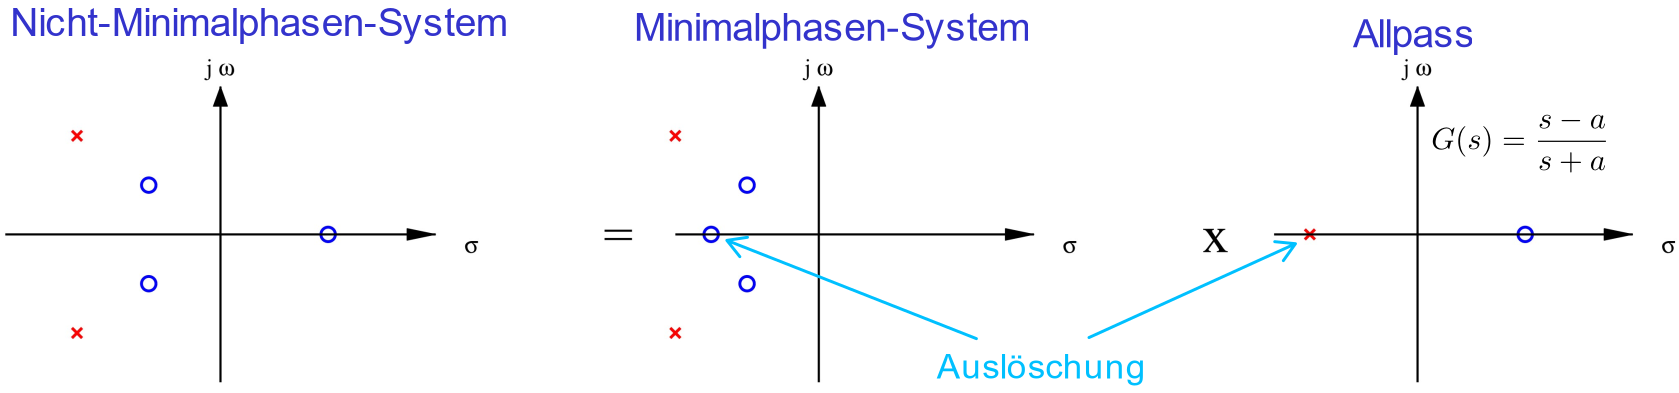
\includegraphics[width=\columnwidth]{images/beispiel_minimalphasensystem.png}




        \section{Bodediagramm}

Beispiele verschiedener Bodediagramme und zugehötiger Pol-Nullstellen-Diagramme \\
siehe Skript, Kapitel 5.4.3 (S. 222)


\subsection{Bodediagramme mit Matlab}

\lstinputlisting{snippets/bode.m}


\subsection{Approximationen im Bodediagramm}{230}

\subsubsection{Pol im Ursprung}

\begin{minipage}[t]{0.48\columnwidth}
    $$ H(s) = \frac{\alpha}{s} \cbl{= \frac{2}{s}} $$
    \begin{center}
    % Gain
    \begin{tikzpicture}
        [
            scale = 0.4,
            >=latex
        ]
        \begin{axis}
            [
                width=12cm,
                height=4cm,
                xmode=log,
                xmin=0.1, xmax=100, ymin=-20, ymax=20,
                x label style={anchor=west},
                xlabel=Frequency $\omega$,
                y label style={anchor=south},
                ylabel=Gain $\deci \bel$,
                xmajorgrids=true,
                xminorgrids=true,
                ymajorgrids=true
            ]

            \addplot[thick, color=blue, domain=0.1:100]{-20*log10(x)+6};

            \addplot[dashed, color=black, domain=0.1:100]{0};
            \addplot[dashed, color=black, domain=2:2] coordinates {(2, -20) (2, 20)};
        \end{axis}
        
    \end{tikzpicture}


    % Phase
    \begin{tikzpicture}
        [
            scale = 0.4,
            >=latex
        ]
        \begin{axis}
            [
                width=12cm,
                height=4cm,
                xmode=log,
                xmin=0.1, xmax=100, ymin=-3.141, ymax=3.141,
                x label style={anchor=west},
                xlabel=Frequency $\omega$,
                y label style={anchor=south},
                ylabel=Phase $\rad$,
                ytick={-3.14, -1.57, 0, 1.57, 3.14},
                yticklabels={$-\pi$, $-\frac{\pi}{2}$, $0$, $\frac{\pi}{2}$, $\pi$},
                xmajorgrids=true,
                xminorgrids=true,
                ymajorgrids=true
            ]
            
            \addplot[thick, color=blue, domain=0.1:100]{-1.57};     

        \end{axis}
            
    \end{tikzpicture}
\end{center}


\end{minipage}
\hfill
\begin{minipage}[t]{0.48\columnwidth}
    \myul{Betrag zeichnen}
        \begin{enumerate}
            \item Waagrechte Gerade fein einzeichnen\\bei $0 \, \deci \bel$
            \item Senkrechte Gerade fein einzeichnen\\bei $\omega = \alpha$
            \item Gerade mit $-20 \, \frac{\deci \bel}{\Dek}$ durch Schnittpunkt der beiden feinen Geraden einzeichnen\\
        \end{enumerate}
    
    \myul{Phase zeichnen}
        \begin{enumerate}
            \item Waagrechte Gerade durch $-\frac{\pi}{2}$
        \end{enumerate}
\end{minipage}


\subsubsection{Nullstelle im Ursprung}

\begin{minipage}[t]{0.48\columnwidth}
    $$ H(s) = \alpha \cdot s \cbl{= 3\cdot s} $$
    \begin{center}
    % Gain
    \begin{tikzpicture}
        [
            scale = 0.4,
            >=latex
        ]
        \begin{axis}
            [
                width=12cm,
                height=4cm,
                xmode=log,
                xmin=0.1, xmax=100, ymin=-20, ymax=20,
                x label style={anchor=west},
                xlabel=Frequency $\omega$,
                y label style={anchor=south},
                ylabel=Gain $\deci \bel$,
                xmajorgrids=true,
                xminorgrids=true,
                ymajorgrids=true
            ]

            \addplot[thick, color=blue, domain=0.1:100]{20*log10(x)-6};

            \addplot[dashed, color=black, domain=0.1:100]{0};
            \addplot[dashed, color=black, domain=2:2] coordinates {(2, -20) (2, 20)};
        \end{axis}
        
    \end{tikzpicture}


    % Phase
    \begin{tikzpicture}
        [
            scale = 0.4,
            >=latex
        ]
        \begin{axis}
            [
                width=12cm,
                height=4cm,
                xmode=log,
                xmin=0.1, xmax=100, ymin=-3.141, ymax=3.141,
                x label style={anchor=west},
                xlabel=Frequency $\omega$,
                y label style={anchor=south},
                ylabel=Phase $\rad$,
                ytick={-3.14, -1.57, 0, 1.57, 3.14},
                yticklabels={$-\pi$, $-\frac{\pi}{2}$, $0$, $\frac{\pi}{2}$, $\pi$},
                xmajorgrids=true,
                xminorgrids=true,
                ymajorgrids=true
            ]
            
            \addplot[thick, color=blue, domain=0.1:100]{1.57};                 
        \end{axis}
            
    \end{tikzpicture}
\end{center}


\end{minipage}
\hfill
\begin{minipage}[t]{0.48\columnwidth}
    \myul{Betrag zeichnen}
        \begin{enumerate}
            \item Waagrechte Gerade fein einzeichnen\\bei $0 \, \deci \bel$
            \item Senkrechte Gerade fein einzeichnen\\bei $\omega = \frac{1}{\alpha}$
            \item Gerade mit $+20 \, \frac{\deci \bel}{\Dek}$ durch Schnittpunkt der beiden feinen Geraden einzeichnen\\
        \end{enumerate}
    
    \myul{Phase zeichnen}
        \begin{enumerate}
            \item Waagrechte Gerade durch $+\frac{\pi}{2}$
        \end{enumerate}
\end{minipage}

\subsubsection{Reeller Pol}

\begin{minipage}[t]{0.48\columnwidth}
    $$ H(s) = \frac{\alpha}{s + \alpha} = \frac{1}{\frac{s}{\alpha} + 1} \cbl{= \frac{4}{s + 4}} $$
    \begin{center}
    % Gain
    \begin{tikzpicture}
        [
            scale = 0.4,
            >=latex
        ]
        \begin{axis}
            [
                width=12cm,
                height=4cm,
                xmode=log,
                xmin=0.1, xmax=1000, ymin=-40, ymax=10,
                x label style={anchor=west},
                xlabel=Frequency $\omega$,
                y label style={anchor=south},
                ylabel=Gain $\deci \bel$,
                ytick={-40, -30, -20, -10, 0, 10},
                yticklabels={-40, -30, -20, -10, 0, 10},
                xmajorgrids=true,
                xminorgrids=true,
                ymajorgrids=true
            ]

            \addplot[thick, color=blue, domain=0.1:4]{0};  
            \addplot[thick, color=blue, domain=4:1000]{-20*log10(x)+12};   
            
            \addplot[dashed, color=black, domain=4:4]coordinates {(4, -40) (4, 10)};  
        \end{axis}
        
    \end{tikzpicture}


    % Phase
    \begin{tikzpicture}
        [
            scale = 0.4,
            >=latex
        ]
        \begin{axis}
            [
                width=12cm,
                height=4cm,
                xmode=log,
                xmin=0.1, xmax=1000, ymin=-3.141, ymax=3.141,
                x label style={anchor=west},
                xlabel=Frequency $\omega$,
                y label style={anchor=south},
                ylabel=Phase $\rad$,
                ytick={-3.14, -1.57, 0, 1.57, 3.14},
                yticklabels={$-\pi$, $-\frac{\pi}{2}$, $0$, $\frac{\pi}{2}$, $\pi$},
                xmajorgrids=true,
                xminorgrids=true,
                ymajorgrids=true
            ]
            
            \addplot[thick, color=blue, domain=0.1:0.4]{0};  
            \addplot[thick, color=blue] coordinates{(0.4, 0) (40, -1.57)};   
            \addplot[thick, color=blue, domain=40:1000]{-1.57};  
            
            \addplot[dashed, color=black, domain=4:4] coordinates {(4, -3.14) (4, 3.14)};  
            \addplot[dashed, color=black, domain=0.1:1000]{-0.79};  

        \end{axis}
            
    \end{tikzpicture}
\end{center}


\end{minipage}
\hfill
\begin{minipage}[t]{0.48\columnwidth}
    \myul{Betrag zeichnen}
    \begin{enumerate}
        \item 0 $\text{dB}$ von $\omega=0$ bis $\omega=\alpha$
        \item $-20\frac{\deci \bel}{\Dek}$ einzeichnen ab $\omega = \alpha$\\
    \end{enumerate}

    \myul{Phase zeichnen}
    \begin{enumerate}
        \item $0$ bis $\omega = \frac{\alpha}{10}$
        \item $-\frac{\pi}{2}$ ab $\omega = 10\cdot \alpha$
        \item Gerade zwischen beiden Geraden 
        \item ($-\frac{\pi}{4}$ bei $\omega=\alpha$)
    \end{enumerate}

\end{minipage}


\subsubsection{Reelle Nullstelle}

\begin{minipage}[t]{0.48\columnwidth}
    $$ H(s) = \frac{s + \alpha}{\alpha} = \frac{s}{\alpha} + 1 \cbl{= \frac{s + 5}{5}} $$
    \begin{center}
    % Gain
    \begin{tikzpicture}
        [
            scale = 0.4,
            >=latex
        ]
        \begin{axis}
            [
                width=12cm,
                height=4cm,
                xmode=log,
                xmin=0.1, xmax=1000, ymin=-10, ymax=40,
                x label style={anchor=west},
                xlabel=Frequency $\omega$,
                y label style={anchor=south},
                ylabel=Gain $\deci \bel$,
                ytick={-10, 0, 10, 20, 30, 40},
                yticklabels={-10, 0, 10, 20, 30, 40},
                xmajorgrids=true,
                xminorgrids=true,
                ymajorgrids=true
            ]

            \addplot[thick, color=blue, domain=0.1:5]{0};  
            \addplot[thick, color=blue, domain=5:1000]{20*log10(x)-14};   
            
            \addplot[dashed, color=black, domain=5:5]coordinates {(5, -10) (5, 40)};  

        \end{axis}
        
    \end{tikzpicture}


    % Phase
    \begin{tikzpicture}
        [
            scale = 0.4,
            >=latex
        ]
        \begin{axis}
            [
                width=12cm,
                height=4cm,
                xmode=log,
                xmin=0.1, xmax=1000, ymin=-3.141, ymax=3.141,
                x label style={anchor=west},
                xlabel=Frequency $\omega$,
                y label style={anchor=south},
                ylabel=Phase $\rad$,
                ytick={-3.14, -1.57, 0, 1.57, 3.14},
                yticklabels={$-\pi$, $-\frac{\pi}{2}$, $0$, $\frac{\pi}{2}$, $\pi$},
                xmajorgrids=true,
                xminorgrids=true,
                ymajorgrids=true
            ]
            
            \addplot[thick, color=blue, domain=0.1:0.5]{0};  
            \addplot[thick, color=blue] coordinates{(0.5, 0) (50, 1.57)};   
            \addplot[thick, color=blue, domain=50:1000]{1.57};  
            
            \addplot[dashed, color=black, domain=5:5] coordinates {(5, -3.14) (5, 3.14)};  
            \addplot[dashed, color=black, domain=0.1:1000]{0.79};                 
        \end{axis}
            
    \end{tikzpicture}
\end{center}
\end{minipage}
\hfill
\begin{minipage}[t]{0.48\columnwidth}

    \myul{Betrag zeichnen}
    \begin{enumerate}
        \item 0 $\text{dB}$ von $\omega=0$ bis $\omega=\alpha$
        \item $+20\frac{\deci \bel}{\Dek}$ einzeichnen ab $\omega = \alpha$\\
    \end{enumerate}

    \myul{Phase zeichnen}
    \begin{enumerate}
        \item $0$ bis $\omega = \frac{\alpha}{10}$
        \item $+\frac{\pi}{2}$ ab $\omega = 10\cdot \alpha$
        \item Gerade zwischen beiden Geraden 
        \item ($+\frac{\pi}{4}$ bei $\omega=\alpha$)
    \end{enumerate}
\end{minipage}
    

\subsubsection{Konjugiert-komplexe Pole}

\begin{minipage}[t]{0.48\columnwidth}
    \raggedright
    \begin{center}
        Voraussetzung: $\abs{q_p} > \frac{1}{2}$
    \end{center}
    $$ H(s) = \frac{\omega_p^2}{s^2 + s \frac{\omega_p}{q_p} + \omega_p^2} \cbl{= \frac{2^2}{s^2 + s \frac{2}{3} + 2^2}} $$

    \begin{center}
    % Gain
    \begin{tikzpicture}
        [
            scale = 0.4,
            >=latex
        ]
        \begin{axis}
            [
                width=12cm,
                height=4cm,
                xmode=log,
                xmin=0.1, xmax=100, ymin=-20, ymax=20,
                x label style={anchor=west},
                xlabel=Frequency $\omega$,
                y label style={anchor=south},
                ylabel=Gain $\deci \bel$,
                xmajorgrids=true,
                xminorgrids=true,
                ymajorgrids=true
            ]

            \addplot[thick, color=blue, domain=0.1:100]{40};
        \end{axis}
        
    \end{tikzpicture}


    % Phase
    \begin{tikzpicture}
        [
            scale = 0.4,
            >=latex
        ]
        \begin{axis}
            [
                width=12cm,
                height=4cm,
                xmode=log,
                xmin=0.1, xmax=100, ymin=-3.141, ymax=3.141,
                x label style={anchor=west},
                xlabel=Frequency $\omega$,
                y label style={anchor=south},
                ylabel=Phase $\rad$,
                ytick={-3.14, -1.57, 0, 1.57, 3.14},
                yticklabels={$-\pi$, $-\frac{\pi}{2}$, $0$, $\frac{\pi}{2}$, $\pi$},
                xmajorgrids=true,
                xminorgrids=true,
                ymajorgrids=true
            ]
            
            \addplot[thick, color=blue, domain=0.1:100]{0};                 
        \end{axis}
            
    \end{tikzpicture}
\end{center}
\end{minipage}
\hfill
\begin{minipage}[t]{0.48\columnwidth}
    \myul{Betrag zeichnen}
        \begin{enumerate}
            \item 0 $\text{dB}$ von $\omega=0$ bis $\omega=\frac{\omega_p}{2}$
            \item $-40\frac{\text{dB}}{\text{Dek}}$ fein einzeichnen ab $\omega_p$\\
            $\rightarrow$ stark zeichnen ab $\omega = 2 \cdot \omega_p$
            \item Maximalwert $= 20\cdot \log_{10}(q_p)$ bei $\omega_p$
            \item Gerade von $\omega=\frac{\omega_p}{2}$ zu Maximalwert 
            \item Gerade von Maximalwert zu $\omega = 2 \cdot \omega_p$\\
        \end{enumerate}
    \myul{Phase zeichnen}
        \begin{enumerate}
            \item 0 bis $\omega < \frac{\omega_p}{10^{\frac{1}{2 q_p}}}$
            \item $- \pi$ ab $\omega > \omega_p \cdot 10^{\frac{1}{2 q_p}}$
            \item Gerade zwischen $0$ und $\pi$ Geraden
            \item ($- \frac{\pi}{2}$ bei $\omega = \omega_p$)
        \end{enumerate}
\end{minipage}


\subsubsection{Konjugiert-komplexe Nullstellen} 

\begin{minipage}[t]{0.48\columnwidth}
    \raggedright
    \begin{center}
        Voraussetzung: $\abs{q_z} > \frac{1}{2}$
    \end{center}
    $$ H(s) = \frac{s^2 + s \frac{\omega_z}{q_z} + \omega_z^2}{\omega_z^2} \cbl{= \frac{s^2 + s \frac{2}{3} + 2^2}{2^2}} $$

    \begin{center}
    % Gain
    \begin{tikzpicture}
        [
            scale = 0.4,
            >=latex
        ]
        \begin{axis}
            [
                width=12cm,
                height=4cm,
                xmode=log,
                xmin=0.1, xmax=100, ymin=-20, ymax=20,
                x label style={anchor=west},
                xlabel=Frequency $\omega$,
                y label style={anchor=south},
                ylabel=Gain $\deci \bel$,
                xmajorgrids=true,
                xminorgrids=true,
                ymajorgrids=true
            ]

            \addplot[thick, color=blue, domain=0.1:100]{40};
        \end{axis}
        
    \end{tikzpicture}


    % Phase
    \begin{tikzpicture}
        [
            scale = 0.4,
            >=latex
        ]
        \begin{axis}
            [
                width=12cm,
                height=4cm,
                xmode=log,
                xmin=0.1, xmax=100, ymin=-3.141, ymax=3.141,
                x label style={anchor=west},
                xlabel=Frequency $\omega$,
                y label style={anchor=south},
                ylabel=Phase $\rad$,
                ytick={-3.14, -1.57, 0, 1.57, 3.14},
                yticklabels={$-\pi$, $-\frac{\pi}{2}$, $0$, $\frac{\pi}{2}$, $\pi$},
                xmajorgrids=true,
                xminorgrids=true,
                ymajorgrids=true
            ]
            
            \addplot[thick, color=blue, domain=0.1:100]{0};                 
        \end{axis}
            
    \end{tikzpicture}
\end{center}
\end{minipage}
\hfill
\begin{minipage}[t]{0.48\columnwidth}
    \myul{Betrag zeichnen}
        \begin{enumerate}
            \item 0 $\text{dB}$ von $\omega=0$ bis $\omega=\frac{\omega_z}{2}$
            \item $+40\frac{\text{dB}}{\text{Dek}}$ fein einzeichnen ab $\omega_z$\\
            $\rightarrow$ stark zeichnen ab $\omega = 2 \cdot \omega_z$
            \item Minimalwert $= -20\cdot \log_{10}(q_z)$ bei $\omega_z$
            \item Gerade von $\omega=\frac{\omega_z}{2}$ zu Miniimalwert 
            \item Gerade von Minimalwert zu $\omega = 2 \cdot \omega_z$\\
        \end{enumerate}
    \myul{Phase zeichnen}
        \begin{enumerate}
            \item 0 bis $\omega < \frac{\omega_z}{10^{\frac{1}{2 q_z}}}$
            \item $+ \pi$ ab $\omega > \omega_z \cdot 10^{\frac{1}{2 q_z}}$
            \item Gerade zwischen $0$ und $- \pi$ Geraden
            \item ($\frac{\pi}{2}$ bei $\omega = \omega_z$)\\
        \end{enumerate}
\end{minipage}

\textbf{Hinweis: Berechnungs-Tabelle aus Skript, S. 235} 

\begingroup
\renewcommand{\arraystretch}{2}
\setlength{\tabcolsep}{0mm}
\scalebox{0.33}{
\Huge
\begin{tabularx}{3\columnwidth}{rp{1mm}V{3}*{17}{C}}
    \rowcolor{subsectioncolor!30}$\bm{q_p}$ && $0.5$ & $1$ & $1.5$ & $2$ & $3$ & $4$ & $5$ & $6$ & $8$ & $10$ & $20$ & $50$ & $100$ \\
    \hline
    $\bm{10^{\frac{1}{2 q_p}}}$     && $10$ & $3.16$ & $2.15$ & $1.78$ & $1.47$ & $1.33$ & $1.26$ & $1.21$ & $1.15$ & $1.12$ & $1.06$ & $1.02$ & $1.01$ \\
    \hline
    $\bm{10^{- \frac{1}{2 q_p}}}$   && $0.1$ & $0.316$ & $0.464$ & $0.562$ & $0.681$ & $0.750$ & $0.794$ & $0.825$ & $0.866$ & $0.891$ & $0.944$ & $0.977$ & $0.989$ \\
\end{tabularx}}
\endgroup
\renewcommand{\arraystretch}{1}

\vspace{0.2cm}

% nicht ändern
\begin{minipage}[t]{0.48\columnwidth}
    \raggedright
    \subsubsection{Konstanter Faktor}

    \begin{outline}
        \1 $H(s) = \alpha \cdot e^{\jimg \beta} \cbl{= 3 \cdot e^{\jimg \frac{\pi}{2}}}$
            \2 Betrag $= 20 \cdot \log_{10}(\alpha) = \const$
            \2 Phase $= \beta = \const$
    \end{outline}
    
    \begin{center}
    % Gain
    \begin{tikzpicture}
        [
            scale = 0.4,
            >=latex
        ]
        \begin{axis}
            [
                width=12cm,
                height=4cm,
                xmode=log,
                xmin=0.1, xmax=100, ymin=-20, ymax=20,
                x label style={anchor=west},
                xlabel=Frequency $\omega$,
                y label style={anchor=south},
                ylabel=Gain $\deci \bel$,
                xmajorgrids=true,
                xminorgrids=true,
                ymajorgrids=true
            ]

            % K_0
            \addplot[thick, color=blue, domain=0.1:100]{20*log10(3)};
        \end{axis}
        
    \end{tikzpicture}


    % Phase
    \begin{tikzpicture}
        [
            scale = 0.4,
            >=latex
        ]
        \begin{axis}
            [
                width=12cm,
                height=4cm,
                xmode=log,
                xmin=0.1, xmax=100, ymin=-3.141, ymax=3.141,
                x label style={anchor=west},
                xlabel=Frequency $\omega$,
                y label style={anchor=south},
                ylabel=Phase $\rad$,
                ytick={-3.14, -1.57, 0, 1.57, 3.14},
                yticklabels={$-\pi$, $-\frac{\pi}{2}$, $0$, $\frac{\pi}{2}$, $\pi$},
                xmajorgrids=true,
                xminorgrids=true,
                ymajorgrids=true
            ]
            
            % K_0
            \addplot[thick, color=blue, domain=0.1:100]{1.57};     

        \end{axis}
            
    \end{tikzpicture}
\end{center}
\end{minipage}
\hfill
\begin{minipage}[t]{0.48\columnwidth}
    \raggedright
    \subsubsection{Weitere Bemerkungen}

    \begin{outline}
        \1 \textbf{Inverser Frequenzgang:}
            \2 Amplitudengang an $0 \, \deci \bel$-Linie spiegeln
            \2 Phasengang an $0 \, \rad$- bzw. $0 \, \degree$-Linie spiegeln
        \1 \textbf{Serieschaltung von mehreren Teilsystemen}
            \2 Erfolgt durch \textbf{grafische Addition} der einzelnen Systeme
        \1 Bei Knickpunkten ist Approximationsfehler am grössten
    \end{outline}

\end{minipage}


\subsection{Ergänzung: Konjugiert-komplexe Pole und Nullstellen}{228}

Ein Tiefpass 2. Ordnung enthält eine Überhöhung und somit ein absolutes Maximum. 

$$ \text{UTF Tiefpass 2. Ordnung:} \quad H(s) = \frac{\omega_p^2}{s^2 + s \frac{\omega_p}{q_p} + \omega_p^2} $$

\renewcommand{\arraystretch}{2}
\begin{tabular}{ll}
    Frequenz beim Maximum:  & $ \omega_{\rm max} = \omega_p \cdot \sqrt{1 - \frac{1}{2 q_p^2}} = \sqrt{\omega_p^2 - 2 \sigma_p^2}$ \\
    Höhe des Maximums:      & $ \abs{H(\omega_{\rm max})} = \frac{q_p}{\sqrt{1 - \frac{1}{4 q_p^2}}}$ \\
\end{tabular}

\textrightarrow Es gilt: $\omega_{max} \leq \omega_p$


\subsubsection{Spezialfall $q = 1$}

\renewcommand{\arraystretch}{1.5}
\begin{minipage}[c]{0.55\columnwidth}    
    \begin{tabular}{ll}
        Frequenz:  & $ \omega_{\rm max} = \omega_p \cdot \sqrt{1 - \frac{1}{2}} = \frac{\omega_p}{\sqrt{2}}$ \\
        Höhe:      & $ \abs{H(\omega_{\rm max})} = \frac{1}{\sqrt{1 - \frac{1}{4}}} = 1.15$ \\
    \end{tabular}

\end{minipage}
\hfill
\begin{minipage}[c]{0.43\columnwidth}
    


\begin{tikzpicture}
	[
	x=1cm, y=1cm, scale=0.67, font=\footnotesize, >=latex 
	%Voreinstellung für Pfeilspitzen
	]
	
	%Raster im Hintergrund
	%\draw[step=1, gray!50!white, very thin] (0,0) grid (5.5,1.5);
	
	
	%Länge x Achse
	\draw [-latex] (0,0) -- ++(5.5,0) node[right] {$\omega$};
	
	%Länge y Achse
	\draw [-latex] (0,0) -- ++(0,1.5) node[above] {$\left\lvert H\left(\omega\right) \right\rvert $};
	
	%Zahlen auf y-Achse 
	\foreach \y in {0,1}
	\draw[shift={(0,\y)}] (2pt,0pt) -- (-2pt,0pt);
	
	%Zahlen auf x-Achse
	\foreach \x in {0}
	\draw[shift={(\x,0)},color=black] (0pt,2pt) -- (0pt,-2pt);
	
	%gestrichelte linie
	\draw [dashed, gray, thick] (0,1) -- (4,1);		
	\draw [dashed, orange, thick] (3.2,-0.05) -- (3.2,1.2);
	\draw [dashed, red, thick] (4,-0.05) -- (4,1);
	
	%Beschriftungen
	\draw [] (0,1) node[left] {$1$};
	\draw [] (4,0) node[red, below] {$\omega_p$};	
	\draw [] (3.3,0) node[orange, below] {$\omega_{\rm max}$};
	\draw [] (5.1,0.7) node[] {$-40\frac{\deci \bel}{\text{Dek.}} $};

	%Geschwungene Linie
	\draw[thick, blue] plot[smooth] coordinates {(0,1) (2,1.15) (3.3,1.2) (4,1) (5.2,0)};
	
	%Punkte
	\fill [orange] (3.2,1.2) circle (0.06cm);
	\fill [red] (4,1) circle (0.06cm);
	
\end{tikzpicture}
\end{minipage}


\subsubsection{Spezialfall $q = \frac{1}{2}$}

\begin{minipage}[c]{0.55\columnwidth}
    \begin{tabular}{ll}
            Frequenz:  & $ \omega_{\rm max} = \omega_p \cdot \sqrt{1 - \frac{1}{2 \big(\frac{1}{2} \big)^2 }}$ \\
                       & $ = \omega_p \cdot \sqrt{1-2} \in \mathbb{C}$ \\
            Höhe:      & $ \abs{H(\omega_{\rm max})} = \infty$ \\   % CHECK: macht das Sinn???
    \end{tabular}
\end{minipage}
\hfill
\begin{minipage}[c]{0.43\columnwidth}
    \begin{tikzpicture}
	[
	x=1cm, y=1cm, scale=0.6, font=\footnotesize, >=latex 
	%Voreinstellung für Pfeilspitzen
	]
	
	%Raster im Hintergrund
	%\draw[step=0.1, gray!50!white, very thin] (0,0) grid (5.5,2.5);
	%\draw[step=1, gray!80!white, thin] (0,0) grid (5.5,2.5);
	
	%Länge x Achse
	\draw [-latex] (0,0) -- ++(5.5,0) node[right] {$\omega$};
	
	%Länge y Achse
	\draw [-latex] (0,0) -- ++(0,2.5) node[above] {$\left\lvert H\left(\omega\right) \right\rvert $};
	
	%Zahlen auf y-Achse 
	\foreach \y in {0,1,2}
	\draw[shift={(0,\y)}] (2pt,0pt) -- (-2pt,0pt);
	
	%Zahlen auf x-Achse
	\foreach \x in {0}
	\draw[shift={(\x,0)},color=black] (0pt,2pt) -- (0pt,-2pt);
	
	%gestrichelte linie
	\draw [dashed, gray, thick] (0,1) -- (4,1);		
	\draw [dashed, red, thick] (4,-0.05) -- (4,1);
	
	%Beschriftungen
	\draw [] (0,2) node[left] {$0 \, \deci \bel$};
	\draw [] (0,1) node[left] {$6 \, \deci \bel$};
	\draw [] (4,0) node[red, below] {$\omega_p$};	
	\draw [] (4,1.8) node[] {negative Überhöhung};	

	%Geschwungene Linie
	\draw[thick, blue] plot[smooth] coordinates {(0,2) (1,1.94) (2,1.75) (3,1.44) (4,1) (4.6,0.57) (5.2,0)};
	\draw [-latex, thick] (4,1.6) -- (4,1.1);

	%Punkte

	\fill [red] (4,1) circle (0.06cm);
	
\end{tikzpicture}


\end{minipage}


\subsubsection{Spezialfall $q =\frac{1}{\sqrt{2}}$}

\begin{minipage}[c]{0.55\columnwidth}

    \begin{tabular}{ll}
        Frequenz:   & $ \omega_{\rm max} = 0$ \\
        Höhe:       & $ \abs{H(\omega_{\rm max})} = q_p = \frac{1}{\sqrt{2}}$ \textrightarrow\ $3 \, \deci \bel$ \\
    \end{tabular}
    \renewcommand{\arraystretch}{2}
\end{minipage}
\hfill
\begin{minipage}[c]{0.43\columnwidth}
        

\begin{tikzpicture}
	[
	x=1cm, y=1cm, scale=0.63, font=\footnotesize, >=latex 
	%Voreinstellung für Pfeilspitzen
	]
	
	%Raster im Hintergrund
	%\draw[step=0.1, gray!50!white, very thin] (0,0) grid (5.5,2.5);
	%\draw[step=1, gray!80!white, thin] (0,0) grid (5.5,2.5);
	
	%Länge x Achse
	\draw [-latex] (0,0) -- ++(5.5,0) node[right] {$\omega$};
	
	%Länge y Achse
	\draw [-latex] (0,0) -- ++(0,2.5) node[above] {$\left\lvert H\left(\omega\right) \right\rvert $};
	
	%Zahlen auf y-Achse 
	\foreach \y in {0,1.5}
	\draw[shift={(0,\y)}] (2pt,0pt) -- (-2pt,0pt);
	\foreach \y in {2}
	\draw[shift={(0,\y)}] (2pt,0pt) -- (-2pt,0pt);
	
	%Zahlen auf x-Achse
	\foreach \x in {0}
	\draw[shift={(\x,0)},color=black] (0pt,2pt) -- (0pt,-2pt);
	
	%gestrichelte linie
	\draw [dashed, gray, thick] (0,1.5) -- (4,1.5);		
	\draw [dashed, red, thick] (4,-0.05) -- (4,1.5);
	
	%Beschriftungen
	\draw [] (0,2) node[left] {$0 \, \deci \bel$};
	\draw [] (0,1.5) node[left] {$3 \, \deci \bel$};
	\draw [] (4,0) node[red, below] {$\omega_p$};	
	\draw [] (2,2.3) node[] {maximal flach};	

	%Geschwungene Linie
	\draw[thick, blue] plot[smooth] coordinates {(0,2) (1,1.95) (2,1.85) (3,1.7) (4,1.5) (4.7,1.24) (5.4,0.9)};
	
	\draw [-latex, thick] (1,2.25) -- (0.1,2.05);

	%Punkte
	\fill [red] (4,1.5) circle (0.06cm);
	
\end{tikzpicture}


\end{minipage}
\renewcommand{\arraystretch}{1}
        \section{Stabilität im Bodediagramm}

\fbox{\parbox{0.95\columnwidth}{
Es gilt, dass wenn der \textbf{offene} Regelkreis $H(s)$ nur Pole in der linken $s$-Halbebene hat (und höchstens zwei Pole 
im Ursprung bei $s = 0$), der \textbf{geschlossene} Regelkreis genau dann \textbf{asymptotisch stabil} ist, wenn $H(\jimg \omega)$
für die \textbf{Durchgangsfrequenz} $\omega_D$ bei der die Amplitude $20 \cdot \log_{10}(|H(\jimg \omega_D)|) = 0 \, \deci \bel$
ist, und eine Phase $> - \pi$ hat. \\
\textrightarrow\ Amplitudenrand und Phasenrand müssen $> 0$ sein, damit das System stabil ist!
}}


\subsection{Amplitudenrand und Phasenrand }

\begin{outline}
    \1 \textbf{Amplitudenrand (Verstärkungsreserve)}
        \2 Abstand des Amplitudengangs zur $0 \, \deci \bel$-Linie bei der Kreisfrequenz $\omega$, bei der die Phase 
        gleich $- \pi$ bzw. $- 180 \degree$ ist.
    \1 \textbf{Phasenrand ( Phasenreserve)}
        \2 Abstand des Phasengangs zur $- \pi$-Linie bei der Kreisfrequenz $\omega$, bei der die Amplitude 
        gleich $0 \, \deci \bel$ ist.
\end{outline}


\subsection{Amplitudenrand und Phasenrand im Bodediagramm}

\begin{minipage}[c]{0.65\columnwidth}
    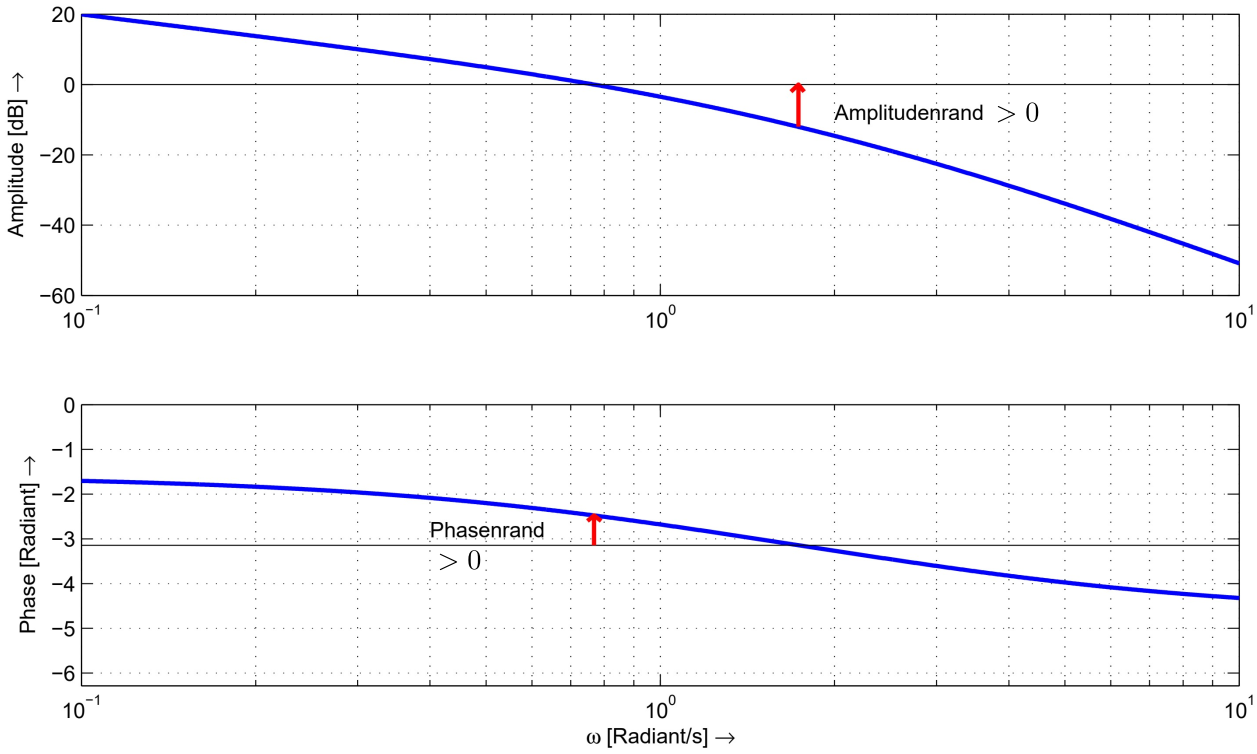
\includegraphics[width=\columnwidth]{images/bode_amplitudenrand_phasenrand.png}
\end{minipage}
\hfill
\begin{minipage}[c]{0.32\columnwidth}
    Das System ist \textbf{stabil}, da sowohl Amplitudenrand als auch Phasenrand $> 0$ sind.
\end{minipage}


        \section{Ortskurve (Nyquist-Diagramm)}{240}

Bei der Ortskurve werden alle komplexen Werte des Frequenzganges in Abhängigkeit der Frequenz $f$ (aufsteigende Werte von $f$) 
in der \textbf{komplexen Ebene} eingetragen. Ortskurven werden vor allem in der Regelungstechnik dazu verendet, um die 
\textbf{Stabilität} eines geschlossenen Regelkreises abzuschätzen. \\
Auf die Konstruktion von Ortskurven wird im Modul Regelungstechnik 2 im Detail eingegangen. Darum soll hier nur auf die Beschreibung
im Skirpt (S. 240 - 242) verwiesen werden.

\subsection{Nyquistdiagramme mit MatLab}

\lstinputlisting{snippets/nyquist.m}
        \section{Stabilität im Bodediagramm}

\subsection{Amplitudenrand}


\subsection{Phasenrand}


        \section{Zustandsraumdarstellung (ZRD)}

\textbf{Grundidee:} Differentialgleichung $n.$ Ordnung eines Systems durch ein \textbf{Differentialgleichungssystem} 
von $n$ Gleichungen $1.$ Ordnung darzustellen.


\subsection{Vorteile der ZRD}{253-254}

\begin{itemize}
    \item Innere Systemstabilitäten können erkannt werden, die bei der Untersuchung der UTF 
        nicht festgestellt werden können \textrightarrow\ Einblick in den \textbf{inneren Aufbau} eines Systems
    \item Wichtig in der Regelungstechnik
    \item ZRD hat Vorteile bei der \textbf{numerischen} Behandlung von Systemen
    \item Beschreibung durch \textbf{Energiespeicher}, in der Elektrotechnik $L$ und $C$
    \item \textbf{Nur Integratoren} werden verwendet, keine Differentiatoren
\end{itemize}


\subsection{Zustandsraumdarstellung (ZRD) im Zeitbereich}{255}
\label{ZRD Zeitbereich}

\begin{minipage}[c]{0.4\columnwidth}
    \vspace{-0.3cm}
    
    \begin{empheq}[box=\fbox] {align*}
        \underline{\dot{x}}(t) &= \bm{A} \underline{x}(t) + \bm{B} \underline{u}(t) \\
        \underline{y}(t) &= \bm{C} \underline{x}(t) + \bm{D} \underline{u}(t)
    \end{empheq}

    \begin{tabular}{ll@{}}
        $\underline{u}(t)$   & Eingangsvektor ($m$ Zeilen) \\
        $\underline{x}(t)$   & Zustandsvektor ($n$ Zeilen) \\
        $\underline{y}(t)$   & Ausgangsvektor ($k$ Zeilen) \\
    \end{tabular}
\end{minipage}
\hfill
\begin{minipage}[c]{0.58\columnwidth}
    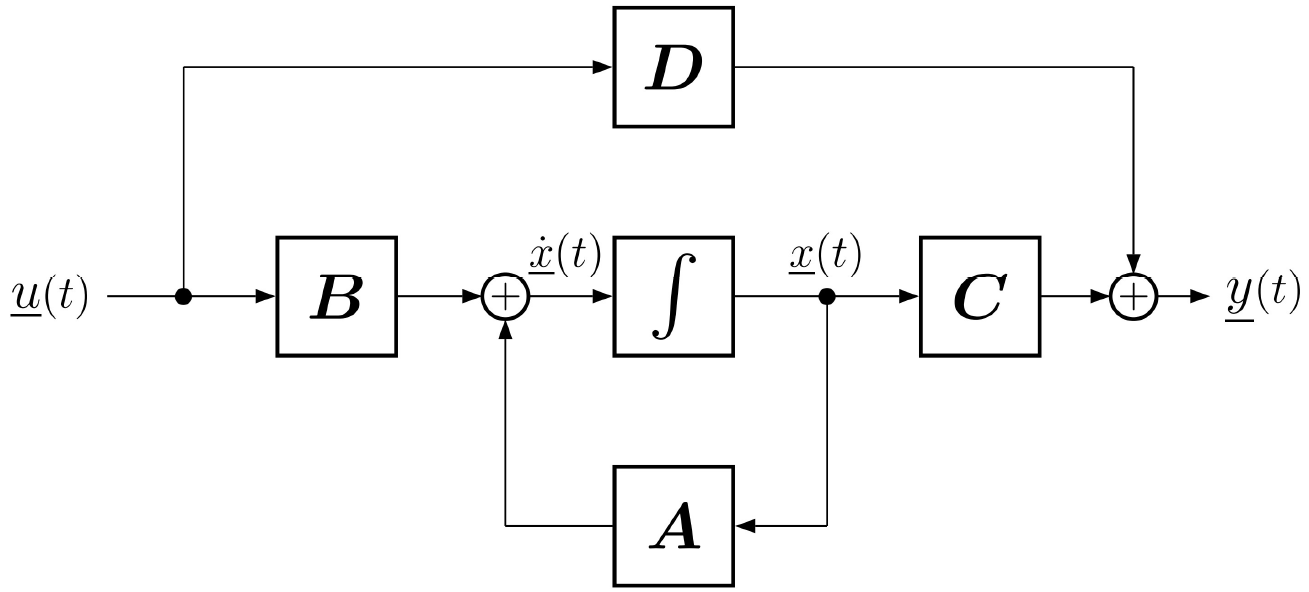
\includegraphics[width=\columnwidth]{images/blockdiagramm_zustandsdarstellung.png}
\end{minipage}


\begin{itemize}
    \item obere Gleichung: \textbf{Zustandsgleichung}
    \item untere Gleichung: \textbf{Ausgangsgleichung}
    \item $\bm{A}$ \textbf{Systemmatrix} ($n \times n$-Matrix) \\
        Sie bestimmt das Verhalten des \textbf{ungestörten Systems} ($\underline{u}(t) = 0$)
        und bestimmt z.B. die innere Stabilität des gesamten Systems.
    \item $\bm{B}$ \textbf{Eingangsmatrix (Steuermatrix)} ($n \times m$-Matrix) \\
        Sie bestimmt die Wirkung der \textbf{Steuergrössen} $\underline{u}(t)$ auf die \textbf{Zustandsgrössen} $\underline{x}(t)$
    \item $\bm{C}$ \textbf{Ausgangsmatrix (Beobachtungsmatrix)} ($k \times n$-Matrix) \\
        Sie kennzeichnet die Abhängigkeit des \textbf{Zustandes} $\underline{x}(t)$ von der beobachtbaren Ausgangsgrösse $\underline{y}(t)$
    \item $\bm{D}$ \textbf{Durchgangsmatrix} ($k \times m$-Matrix) \\
        Sie bestimmt die unmittelbare Wirkung der Eingangsgrösse $\underline{u}(t)$ auf den Ausgang $\underline{y}(t)$
\end{itemize}


\example{ZRD aus Schaltung aufstellen}

\begin{minipage}[c]{0.48\columnwidth}
    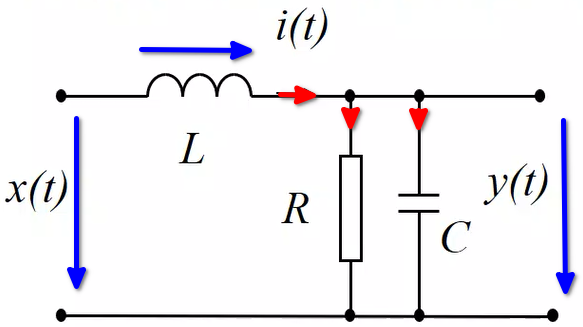
\includegraphics[width=0.9\columnwidth]{images/beispiel_zrd_aus_schaltung.png}
\end{minipage}
\hfill
\begin{minipage}[c]{0.48\columnwidth}
    \begin{itemize}
        \item DGL Induktivität: $\frac{\diff i_L(t)}{\diff t} = \frac{u_L(t)}{L}$ \\
            \textrightarrow\ $u_L(t) = L \cdot \frac{\diff i_L(t)}{\diff t}$
        \item DGL Kapazität: $\frac{\diff u_C(t)}{\diff t} = \frac{i_C(t)}{C}$ \\
        \textrightarrow\ $u_C(t) = \frac{1}{C} \int\limits_{- \infty}^t i(\tau) \, \diff \tau$
    \end{itemize}
\end{minipage}

\begin{minipage}[c]{0.5\columnwidth}
    \begin{empheq}[box=\fbox] {align*}
        \text{Maschen: } & L \cdot \frac{\partial i(t)}{\partial t} + y(t) = x(t) \\
        \text{Knoten: }  & \frac{1}{C} \int\limits_{- \infty}^t \Big( i(\tau) - \frac{y(\tau)}{R} \Big) \, \diff \tau = y(t)
    \end{empheq}
\end{minipage}
\hfill
\begin{minipage}[c]{0.48\columnwidth}
    Beide Gleichungen in ihre differentielle Form bringen (zweite Gleichung ableiten)
\end{minipage}

\begin{minipage}[c]{0.5\columnwidth}
    \begin{align*}
        L \cdot i'(t) + y(t) &= x(t) \\
        i(t) - \frac{y}{R} &= C \cdot y'(t) 
    \end{align*}
\end{minipage}
\hfill
\begin{minipage}[c]{0.48\columnwidth}
    Gleichungen umformen, sodass die ZRD aufgestellt werden kann
\end{minipage}

\begin{minipage}[c]{0.5\columnwidth}
    \begin{align*}
        i'(t) &= - \frac{1}{L} y(t) + \frac{1}{L} x(t) \\
        y'(t) &= \frac{1}{C} i(t) - \frac{1}{RC} y(t) 
    \end{align*}
\end{minipage}
\hfill
\begin{minipage}[c]{0.48\columnwidth}
    \begin{tabular}{ll}
        Zustände:   & $i(t)$, $y(t)$ \\
        Eingang:    & $x(t)$ \\
        Ausgang:    & $\tilde{y}(t) = y(t)$ \\
    \end{tabular}
    
    % \textrightarrow\ Gleichungssystem in Matrixform schreiben
\end{minipage}

\begin{empheq}[box=\fbox] {align*}
    \begin{bmatrix} i'(t) \\ y'(t) \end{bmatrix} &= \underbrace{ \begin{bmatrix} 0 & -\frac{1}{L} \\ \frac{1}{C} & -\frac{1}{RC} \end{bmatrix} }_{\bm{A}}
    \cdot \begin{bmatrix} i(t) \\ y(t) \end{bmatrix} + \underbrace{ \begin{bmatrix} \frac{1}{L} \\ 0 \end{bmatrix} }_{\bm{B}} \cdot x(t) \\
    \tilde{y}(t) &= \underbrace{ \begin{bmatrix} 0 & 1 \end{bmatrix}}_{\bm{C}} \cdot \begin{bmatrix} i(t) \\ y(t) \end{bmatrix} + \underbrace{ \begin{bmatrix} 0 \end{bmatrix} }_{\bm{D}} \cdot x(t)
\end{empheq}


\example{ZRD aus Signalflussdiagramm aufstellen}

Das ZRD zu folgendem System soll aufgestellt werden. Dazu müssen die Matritzen $\bm{A}, \bm{B}, \bm{C}$ und $\bm{D}$ gefunden werden.
$$ \text{Zustandsvektor: }  \underline{q}(t) =  \begin{bmatrix} q_1(t) \\ q_2(t) \\ q_3(t) \end{bmatrix} 
\text{ und dessen Ableitung } \underline{\dot{q}}(t) = \begin{bmatrix} \dot{q}_1(t) \\ \dot{q}_2(t) \\ \dot{q}_3(t) \end{bmatrix} $$
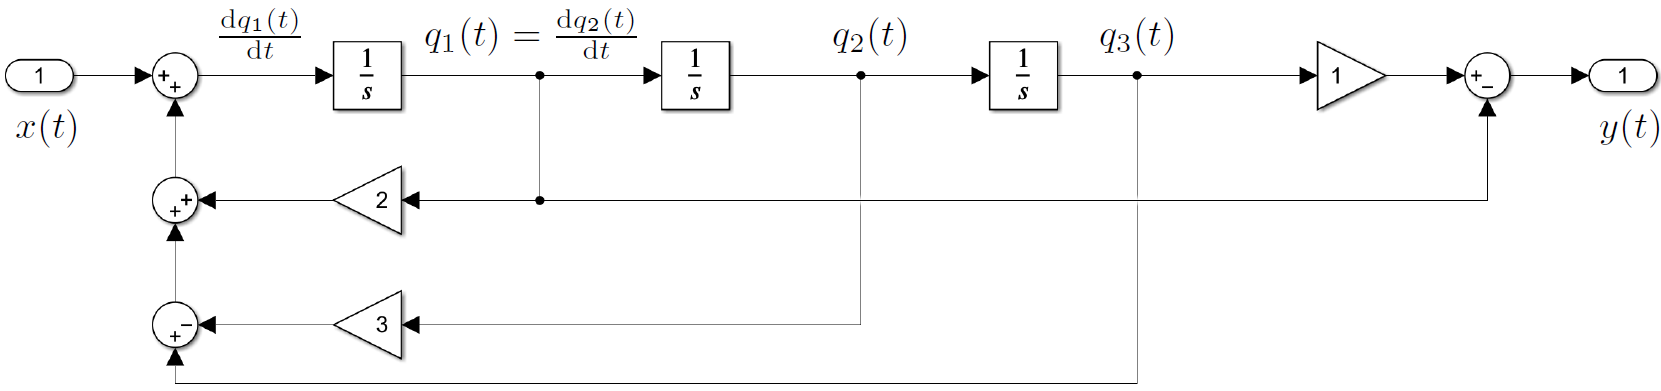
\includegraphics[width=\columnwidth]{images/beispiel_zrd_aus_sfd.png}

\begin{empheq}[box=\fbox] {align*}
    \underbrace{ \begin{bmatrix} \dot{q}_1(t) \\ \dot{q}_2(t) \\ \dot{q}_3(t) \end{bmatrix} }_{\underline{\dot{q}}(t)} &= 
    \underbrace{ \begin{bmatrix} 2 & -3 & 1 \\ 1 & 0 & 0 \\ 0 & 1 & 0 \end{bmatrix} }_{\bm{A}}
    \cdot \underbrace{ \begin{bmatrix} q_1(t) \\ q_2(t) \\ q_3(t) \end{bmatrix} }_{\underline{q}(t)} 
    + \underbrace{ \begin{bmatrix} 1 \\ 0 \\ 0 \end{bmatrix} }_{\bm{B}} \cdot x(t) \\
    y(t) &= \underbrace{ \begin{bmatrix} -1 & 0 & 1 \end{bmatrix}}_{\bm{C}} 
    \cdot \underbrace{ \begin{bmatrix} q_1(t) \\ q_2(t) \\ q_3(t) \end{bmatrix} }_{\underline{q}(t)} 
    + \underbrace{ \begin{bmatrix} 0 \end{bmatrix} }_{\bm{D}} \cdot x(t)
\end{empheq}


\subsection{Zustandsraumdarstellung (ZRD) im Laplace-Bereich}{264}

\begin{minipage}[c]{0.44\columnwidth}
    \vspace{-0.3cm}
    
    \begin{empheq}[box=\fbox] {align*}
        s \underline{X}(s) - x(0) &= \bm{A} \underline{X}(s) + \bm{B} \underline{U}(s) \\
        \underline{Y}(s) &= \bm{C} \underline{X}(s) + \bm{D} \underline{U}(s)
    \end{empheq}

    \begin{tabular}{ll@{}}
        $\underline{U}(s)$   & Eingangsvektor ($m$ Zeilen) \\
        $\underline{X}(s)$   & Zustandsvektor ($n$ Zeilen) \\
        $\underline{Y}(s)$   & Ausgangsvektor ($k$ Zeilen) \\
        $\bm{I}$             & Einheitsmatrix \\
        $\bm{H(s)}$          & Übertragungsmatrix ($k \times m$)\\
    \end{tabular}

\end{minipage}
\hfill
\begin{minipage}[c]{0.54\columnwidth}
    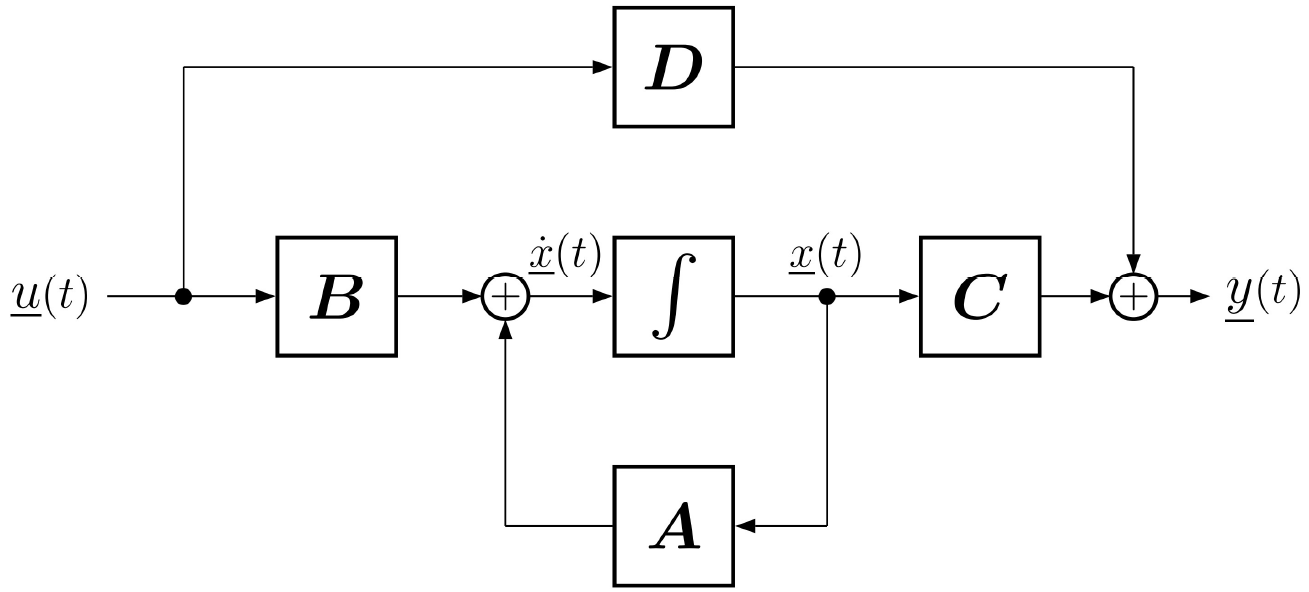
\includegraphics[width=\columnwidth]{images/blockdiagramm_zustandsdarstellung.png}
\end{minipage}

\vspace{0.2cm}
$$ \boxed{ \underline{Y}(s) = \bm{C}(s \bm{I} - \bm{A})^{-1} \underline{x}(0) 
    + \underbrace{(\bm{C}(s \bm{I} - \bm{A})^{-1} \bm{B} + \bm{D} )}_{\bm{H(s)}} \underline{U}(s) } $$

Mit Anfangsbedingungen $x(0) = 0$ ergibt sich folgender Zusammenhang, was der Übertragungsfunktion (UTF) entspricht,
aber im allgemeinen Fall eine \textbf{Matrix} ist.
$$ \boxed{ \underline{Y}(s) = \underbrace{(\bm{C}(s \bm{I} - \bm{A})^{-1} \bm{B} + \bm{D} )}_{\bm{H(s)}} \underline{U}(s) } $$

\textbf{Hinweis:} Aus einem Signalflussdiagramm (SFD) ist es meist sehr einfach, die gesuchten Grössen der ZRD zu finden.


\subsubsection{Übertragungsmatrix und Übertragungsfunktion}{266}

\begin{minipage}[t]{0.48\columnwidth}
    \begin{center}
        \textbf{\myul{Übertragungsmatrix}}
    \end{center}
    \begin{itemize}
        \item MIMO-Systeme
        \item Beschreibung in Matritzenform
            $$ Y(s) = \bm{H(s)} \cdot U(s) $$
        \item  $H(s)$ hat gleiche Grösse (Dimensionen) wie Durchgangsmatrix $\bm{D}$
    \end{itemize}
\end{minipage}
\hfill
\begin{minipage}[t]{0.48\columnwidth}
    \begin{center}
        \textbf{\myul{Übertragungsfunktion}}
    \end{center}
        \begin{itemize}
            \item SISO-Systeme
            \item Matrix-Form wird zu 'normaler' Gleichung
            $$ Y(s) = H(s) \cdot U(s) $$
        \end{itemize}
\end{minipage}


\subsection{Ordnung eines Systems}{256}

Die \textbf{Ordnung} eines Systems definiert die \textbf{kleinste Anzahl von Zustandsgrössen} $x(t)$.
Äquivalent dazu kann die Ordnung eines Systems auch als die \textbf{Anzahl der unabhängigen Energiespeicher} definiert werden.


\subsection{ZRD mit Matlab}

$$ H(s) = \frac{b_i s^i + b_{i-1} s^{i-1} \cdots b_1 s^1 + b_0}{a_i s^i + a_{i-1} s^{i-1} \cdots a_1 s^1 + a_0} $$
\lstinputlisting{snippets/zrd_frequenzbereich.m}


\subsection{Äquivalente Zustandsraumdarstellung (ZRD)}{257}
\label{Äquivalente ZRD}

Mit einer \textbf{Transformationsmatrix} $\bm{T}$ ($n \times n$-Matrix, nicht singulär, $\bm{T T^{-1} = I = T^{-1} T}$) kann man 
\textbf{verschiedenste Zustandsgrössen und Zustandsraumdarstellungen} erhalten, die aber alle ein 
\textbf{identisches Systemverhalten} aufweisen. \\
% Somit kann eine ZRD durch \textbf{verschiedene Schaltungen} realisiert werden, solange diese Schaltungen die 
% \textbf{gleiche Übertragungsfunktion} liefern!

\begin{minipage}[c]{0.4\columnwidth}
    \vspace{-0.3cm}
    
    \begin{empheq}[box=\fbox] {align*}
        \underline{\dot{\xi}}(t) &= \overbrace{ \bm{ T A T}^{-1}}^{\bm{\hat{A}}} \underline{\xi}(t) + \overbrace{\bm{T B}}^{\bm{\hat{B}}}  \underline{u}(t) \\
        \underline{y}(t) &= \underbrace{\bm{C T}^{-1}}_{\bm{\hat{C}}} \underline{\xi}(t) + \underbrace{\bm{D}}_{\bm{\hat{D}}} \underline{u}(t)
    \end{empheq}
\end{minipage}
\hfill
\begin{minipage}[c]{0.58\columnwidth}
    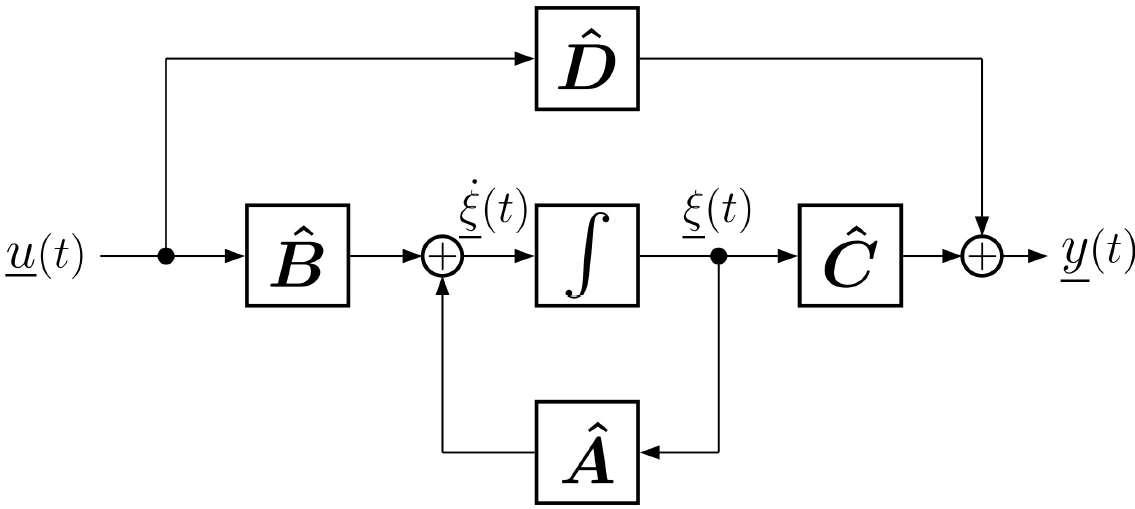
\includegraphics[width=\columnwidth]{images/aequivalente_zrd.png}
\end{minipage}

Die obige ZRD ist \textbf{äquivalent} zur ZRD aus Abschnitt ~\ref{ZRD Zeitbereich} bezüglich $\underline{y}(t)$ und $\underline{u}(t)$.
Die bedeutet, dass die \textbf{Zustandsgrössen} $\underline{\xi}(t)$ und $\underline{x}(t)$ \textbf{willkürlich} gewählt 
werden können, solange $\bm{T}$ nicht singulär ist (Determinante von $\bm{T} \neq 0$) \\

Physikalisch sinnvolle Zustandsgrössen sind:
\begin{itemize}
    \item Spannungen über Kapazitäten
    \item Ströme durch Induktivitäten
\end{itemize}


\subsection[Matrix bm{A} diagonalisieren]{Matrix $\bm{A}$ diagonalisieren}

Oft wird die \textbf{Systemmatrix} $\bm{A}$ diagonalisiert, um \textbf{entkoppelte Zustände} zu erhalten. Anstelle der Matrix
$\bm{\hat{A}} = \bm{ T A T}^{-1}$ wird dann üblicherweise $\bm{A_{\rm diag}}$ verwendet.

\begin{tabular}{ll}
    $\lambda_i$                         & Eigenwerte der Matrix $\bm{A}$ \\
    $\vec{v}_i$                         & Eigenvektoren der Matrix $\bm{A}$ \\
    $\bm{V}$                            & Matrix mit Eigenvektoren von $\bm{A}$ \\
    $\bm{A_{\rm diag}} = \bm{\Lambda}$  & Diagonalisierte Matix $\bm{A}$ mit Eigenwerten $\lambda_i$ auf Diagonale \\
    $\bm{T}$                            & Transformationsmatrix 
\end{tabular}

\begin{minipage}[c]{0.48\columnwidth}
    $$ \boxed{\bm{A_{\rm diag}} = \bm{\Lambda} =  \bm{V}^{-1} \cdot \bm{A} \cdot \bm V} $$
\end{minipage}
\hfill
\begin{minipage}[c]{0.48\columnwidth}
    \begin{empheq}[box=\fbox] {align*}
        \bm{T} &= \bm{V}^{-1} \\
        \bm{T}^{-1} &= \bm{V} 
    \end{empheq}
\end{minipage}


\subsubsection{Vorgehen Matrix diagonalisieren}

\begin{outline}
    \1 Ansatz: $ \bm{A} \cdot \vec{v} = \lambda \cdot \vec{v}$ \textrightarrow\ $(\bm{A} - \lambda \bm{I}) \cdot \vec{v} = \vec{0}$ bzw. 
        $(\lambda \bm{I} - \bm{A}) \cdot \vec{v} = \vec{0}$
    \1 Determinante des charakteristischen Polynoms Null setzen: $\abs{\lambda \bm{I} - \bm{A}} = 0$ \\
        \textrightarrow\ Eigenwerte $\lambda_i$ 
    \1 Für jeden gefundenen Eigenwert müssen Eigenvektoren $\vec{v}_i$ gefunden werden:
        \2 Eigenwert $\lambda_i$ in Gleichungssystem $(\lambda_i \bm{I} - \bm{A}) \cdot \vec{v}_i = \vec{0}$ einsetzen
        \2 Einen Wert von $\vec{v}_i = 1$ wählen und Eigenvektor $\vec{v}_i$ als Spaltenvektor schreiben
    \1 Matrix $\bm{V}$ aus Eigenvektoren 'zusammenbauen'
    \1 Matrix $\bm{\Lambda}$ 'zusammenbauen', indem man Eigenwerte $\lambda_i$ auf Diagonale schreibt
\end{outline}


\subsubsection{Entkoppeltes vs. nicht-entkoppeltes System}

\begin{minipage}[t]{0.4\columnwidth}
    \begin{center}
        \myul{\textbf{Nicht-entkoppeltes System}}
    \end{center}
    $$ \bm{A} = \begin{bmatrix*}[r] -2 & 7 \\ -1 & 6 \end{bmatrix*} $$
    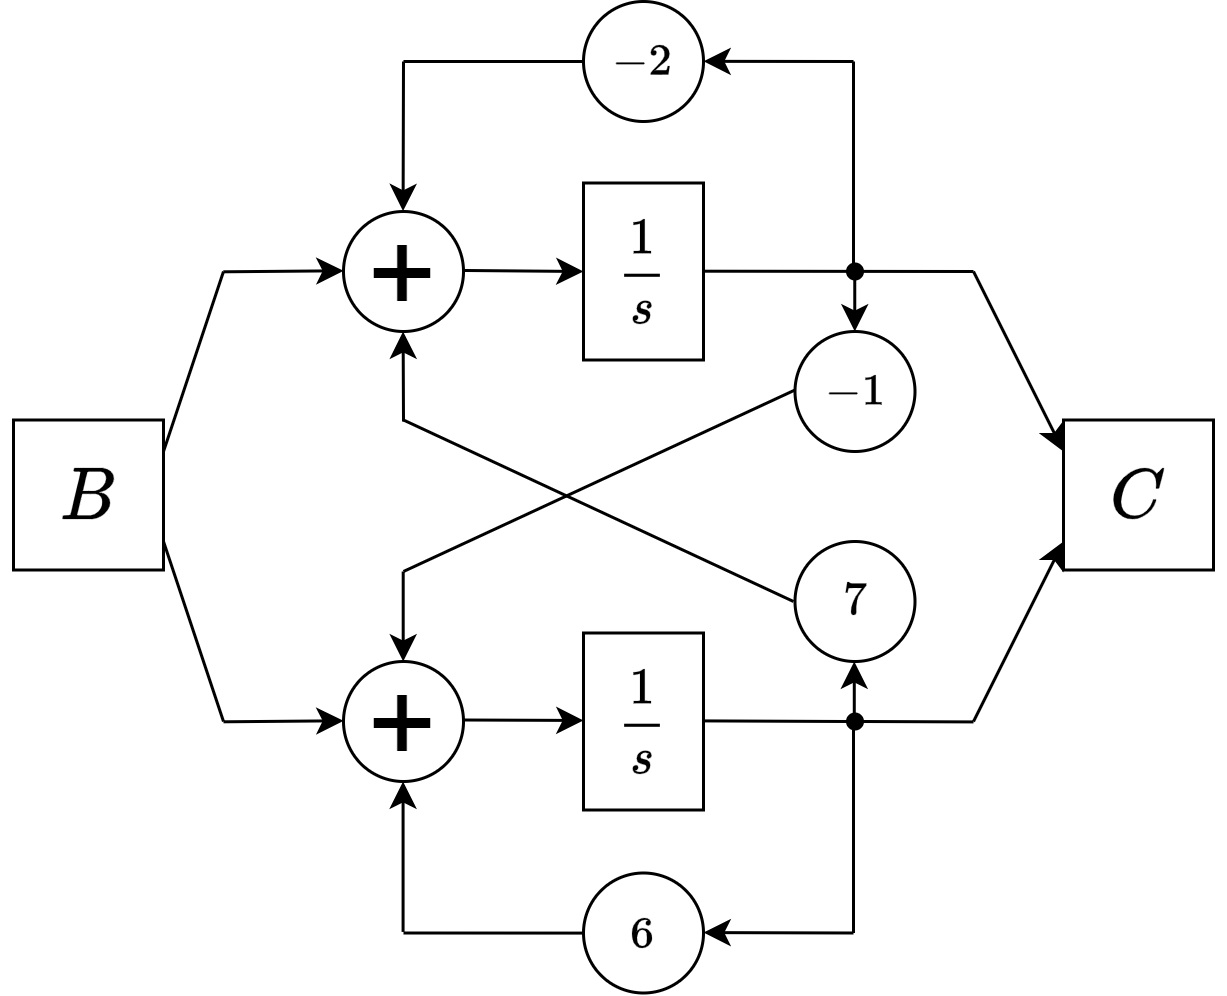
\includegraphics[width=\columnwidth]{images/kreuzform.png}
\end{minipage}
\hfill
\begin{minipage}[t]{0.48\columnwidth}
    \begin{center}
        \myul{\textbf{Entkoppeltes System}}
    \end{center}
    $$ \bm{\hat{A}} = \bm{A_{\rm diag}} = \begin{bmatrix*}[r] -1 & 0 \\ 0 & 5 \end{bmatrix*} $$
    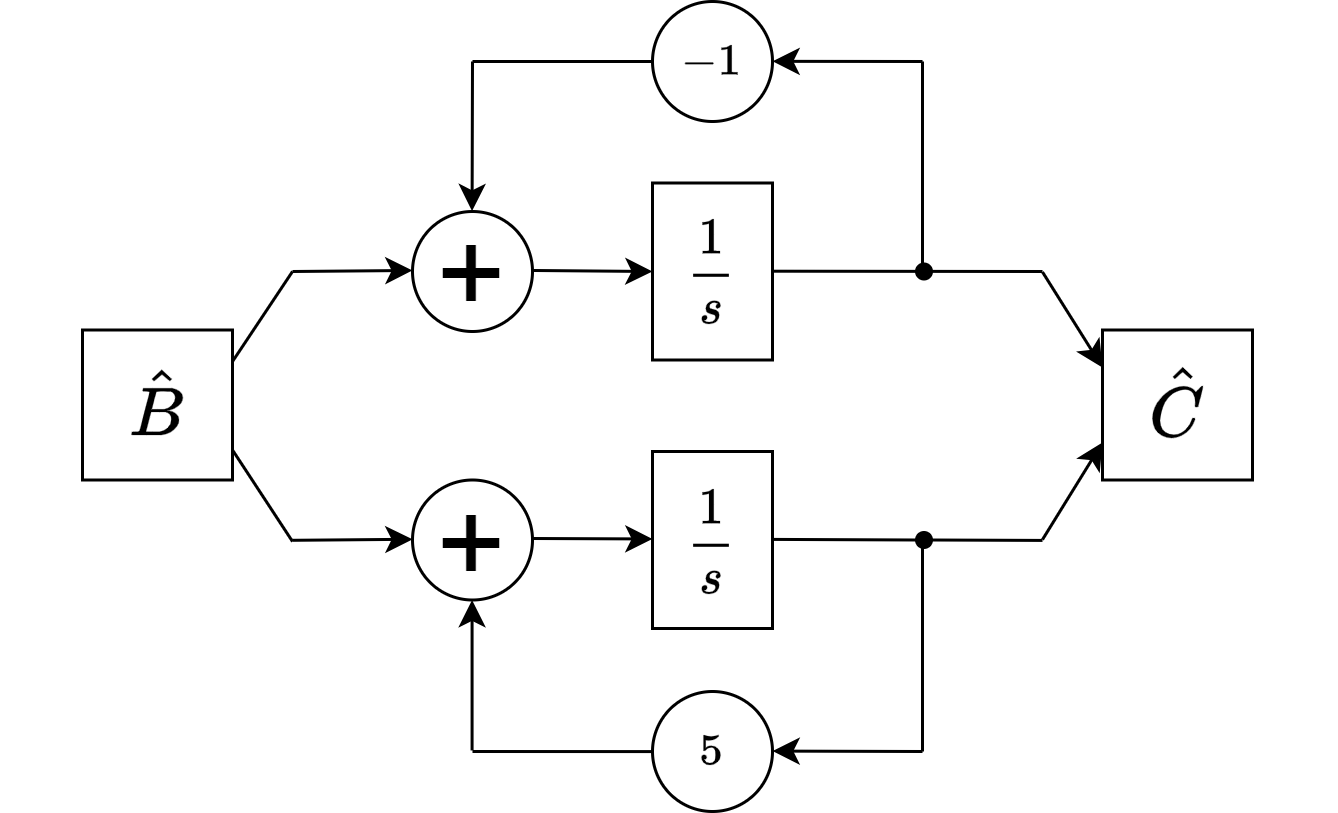
\includegraphics[width=\columnwidth]{images/parallelform.png}
\end{minipage}


\subsection{Einschub -- Lineare Algebra: 2x2 Matrix invertieren}

\begin{minipage}[b]{0.33\columnwidth}
    $$ \bm{A} = 
    \begin{bmatrix*}[r]
        a & b \\
        c & d 
    \end{bmatrix*} $$
\end{minipage}
\hfill
\begin{minipage}[b]{0.66\columnwidth}
    $$ \bm{A}^{-1} = \frac{1}{\det(\bm{A})} \cdot 
    \begin{bmatrix*}[r]
        d & -b \\
        -c & a 
    \end{bmatrix*} \quad \text{ mit } \det(\bm{A}) = ad - bc $$
\end{minipage}


\example{Matrix-Diagonalisierung}{258}

\begin{minipage}[c]{0.25\columnwidth}
    $$ \bm{A} = \begin{bmatrix*}[r]
        -2 & 7 \\
        -1 & 6 
    \end{bmatrix*}$$ 
\end{minipage}
\hfill
\begin{minipage}[c]{0.72\columnwidth}
    $$ \abs{\lambda \bm{I} - \bm{A}} = \begin{vmatrix*}[c]
        \lambda + 2 & -7 \\
        1 & \lambda - 6 
    \end{vmatrix*} = (\lambda + 2) \cdot (\lambda - 6) - 7 \cdot (-1) = 0 $$
\end{minipage}

\textrightarrow\ Mitternachtsformel liefert die Eigenwerte $\lambda_1 = -1$ und $\lambda_2 = 5$

\begin{minipage}[t]{0.56\columnwidth}
    Ersten Eigenwert $\lambda_1 = -1$ in $(\lambda_1 \bm{I} - \bm{A}) \cdot \vec{v}_1 = \vec{0}$ einsetzen
\end{minipage}
\hfill
\begin{minipage}[c]{0.4\columnwidth}
    \begin{align*}
        1 \cdot v_{11} - 7 \cdot v_{21} &= 0 \\
        1 \cdot v_{11} - 7 \cdot v_{21} &= 0 
    \end{align*}
\end{minipage}

\begin{minipage}[c]{0.4\columnwidth}
    Wähle $v_{21} = 1$ \quad \textrightarrow\ $ \vec{v}_1 = \begin{bmatrix*}[r] 7 \\ 1 \end{bmatrix*} $
\end{minipage}
\hfill
\begin{minipage}[c]{0.56\columnwidth}
   Gleichen Vorgehen für zweiten Eigenvektor $\vec{v}_2$
\end{minipage}

\begin{minipage}[c]{0.48\columnwidth}
    $$ \Lambda = \begin{bmatrix} \lambda_1 & 0 \\ 0 & \lambda_2 \end{bmatrix} $$
\end{minipage}
\hfill
\begin{minipage}[c]{0.48\columnwidth}
    $$ \bm{V} = \begin{bmatrix} \vec{v}_1 & \vec{v}_2 \end{bmatrix} = \begin{bmatrix} v_{11} & v_{12} \\ v_{21} & v_{22} \end{bmatrix} $$
\end{minipage}


\subsection{Lösung der ZRD im Zeitbereich}{259-260}
\label{ZRD Lösung Zeitbereich}

Die Zustandsgleichung $\underline{\dot{x}}(t) = \bm{A} \underline{x}(t) + \bm{B} \underline{u}(t)$ ist eine Differentialgleichung.
Sie soll mit dem Ansatz einer Exponentialfunktion gelöst werden. Für Systeme mit nur einem Zustand würde man den Ansatz 
$\underline{x}(t) = e^{at}$ wählen. \\
Da im Allgemeinen Systeme mit mehreren Zuständen betrachtet werden, wird der folgende Ansatz gewählt:

$$ e^{\bm{A} t} = \bm{I} + \bm{A} t + \frac{\bm{A}^2}{2!} t^2 + \cdots + \frac{\bm{A}^k}{k!} t^k + \cdots 
    = \sum\limits_{k=0}^{\infty} \frac{\bm{A}^k t^k}{k!} $$

Der Ansatz ist beschrieben als desser \textbf{Taylor-Reihe.}

Durch einsetzen des Ansatzes in die Zustandsgleichung ergibt sich für den Ausgangsvektor $\underline{y}(t)$ die folgende Lösung
der ZRD im Zeitbereich

$$ \boxed{ \underline{y}(t) = \bm{C} \, \bm{\Phi}(t) \, \underline{x}(0) + 
    \int\limits_0^t \bm{C} \, \bm{\Phi}(t - \tau) \, \bm{B} \, \underline{u}(t) \, \diff \tau + \bm{D} \, \underline{u}(t) } $$

\textbf{Hinweis:} $\bm{\Phi}(t) = e^{\bm{A} t}$ heisst \textbf{Fundamentalmatrix}. 


\subsection{Fundamentalmatrix}{260-263}

Die Fundamentalmatrix (auch Transitionsmatrix genannt) ist definiert als
$$ \boxed{  e^{\bm{A} t} = \bm{\Phi}(t) } $$

Sie wird benötigt, um die Zustandsraumdarstellung im \textbf{Zeitbereich} zu lösen.
Es gibt mehrere Methoden, die quadratische $(n \times n)$ Fundamentalmatrix zu bestimmen


\subsubsection{Methode 1 -- Inverse Laplace-Transformation}

$$ \boxed{ \bm{\Phi}(t) = \mathcal{L}^{-1} \Bigl\{ (s \bm{I} - \bm{A}^{-1})  \Bigr\} } $$


\example{Methode 1 -- Inverse Laplace-Transformation}

Mit der \textbf{Systemmatrix} $\bm{A} = \begin{bmatrix*}[r] -1 & 0 \\ 1 & -2 \end{bmatrix*}$ ergibt sich 
$(s \bm{I} - \bm{A}) = \begin{bmatrix*} s+1 & 0 \\ -1 & s+2 \end{bmatrix*}$

Somit ist $(s \bm{I} - \bm{A})^{-1} = \frac{\begin{bmatrix*} s+1 & 0 \\ -1 & s+2 \end{bmatrix*}}{(s+1)(s+2)} \,
\laplace \, \begin{bmatrix*} e^{-t} & 0 \\ e^{-t} - e^{-2t} & e^{-2t} \end{bmatrix*} = \bm{\Phi}(t)$


\subsubsection{Methode 2 -- Diagonalisierung von $\bm{\Phi}(t) = e^{\bm{A} t}$}

\begin{minipage}[c]{0.6\columnwidth}
    $$ \bm{\Phi}(t) = e^{\bm{A} t} = \underbrace{ 
    \begin{bmatrix*} 
        e^{\lambda_1 t} &                   & \cdots        & 0      \\
                        & e^{\lambda_2 t}   &               & \vdots \\
        \vdots          &                   & \ddots        &        \\
        0               & \cdots            &               & e^{\lambda_n t}
\end{bmatrix*}}_{\bm{\Phi_{\rm diag}(t)}} \cdot \bm{V}^{-1} $$
\end{minipage}
\hfill
\begin{minipage}[c]{0.36\columnwidth}
    Wenn $\bm{A_{\rm diag}} = \bm{V}^{-1} \cdot A \cdot \bm{V}$ ist und $\lambda_i$ die Eigenwerte von $\bm{A}$ sind
\end{minipage}


\subsubsection{Methode 3 -- Spektrale Zerlegung}

\textrightarrow\ Nicht in Vorlesung behandelt


\subsubsection{Methode 4 -- Satz von Cayley-Hamilton}
\textrightarrow\ Nicht in Vorlesung behandelt


\subsubsection{Methode 5 -- Definition der Reihenentwicklung}

% Gemäss Abschnitt ~\ref{ZRD Lösung Zeitbereich} ist die Fundamentalmatrix $\bm{\Phi}(t) = e^{\bm{A} \cdot t}$ als Taylor-Reihe
% definiert.

\begin{minipage}[c]{0.6\columnwidth}
    Die Matrix $\bm{A}$ sei definiert als eine \textbf{Dreiecksmatrix} mit Parameteren $a$ und $c$
\end{minipage}
\hfill
\begin{minipage}[c]{0.38\columnwidth}
    $$ \bm{A} = \begin{bmatrix*} a & 0 \\ 1 & c \end{bmatrix*} $$
\end{minipage}


\begin{minipage}[c]{0.5\columnwidth}
    Die Potenz der Matrix wird berechnet aus
\end{minipage}
\hfill
\begin{minipage}[c]{0.48\columnwidth}
    $$ \bm{A}^k = \begin{bmatrix*} a & 0 \\ 1 & c \end{bmatrix*}^k 
    = \begin{bmatrix*} a^k & 0 \\ \sum\limits_{l=0}^{k-1} a^{k-l-1} c^l  & c^k \end{bmatrix*} $$
\end{minipage}


\subsubsection{Eigenschaften der Fundamentalmatrix $\bm{\Phi(t) = e^{\bm{A} t}$}}

\begin{tabular}{l c l}
    \toprule
    $\bm{\Phi}(0) = \bm{I} $            & & $e^{\bm{A} \cdot 0} = \bm{I}$ \\
    \midrule
    $\bm{\Phi}^{-1}(t) = \bm{\Phi}(-t)$ & & $\big( e^{\bm{A} \cdot t} \big)^{-1} = e^{- \bm{A} \cdot t}$ \\
    \midrule
    $\bm{\Phi}^k(t) = \bm{\Phi}(kt)$    & & $\big( e^{\bm{A} \cdot t} \big)^k = e^{\bm{A} \cdot k \cdot t}$ \\
    \midrule
    $\bm{\Phi}(t_1) \cdot \bm{\Phi}(t_2) = \bm{\Phi}(t_1 + t_2)$                & & $e^{\bm{A} \cdot t_1} \cdot e^{\bm{A} \cdot t_2} = e^{\bm{A} (t_1 + t_2)}$ \\
    \midrule
    $\bm{\Phi}(t_2 - t_1) \cdot \bm{\Phi}(t_1 - t_0) = \bm{\Phi}(t_2 - t_0)$    & & $e^{\bm{A} (t_2 - t_1)} \cdot e^{\bm{A} (t_1 - t_0)} = e^{\bm{A} (t_2 - t_0)}$ \\
    \bottomrule
\end{tabular}

\vspace{0.2cm}
\textbf{Hinweis:} ($\bm{\Phi}(t)$ ist stets invertierbar)


\subsubsection{Fundamentalmatrix in Matlab}

\lstinputlisting{snippets/fundamentalmatrix.m}

% --------------------------------------------------------------------------------------------------

\subsection{Lösung der ZRD im Zeitbereich -- SISO-Systeme}{263}

Die Impulsantwort $h(t)$ eines SISO-Systems ist gegeben durch

\begin{empheq}[box=\fbox] {align*}
    y(t) &= \bm{C} \bm{\Phi}(t) \bm{B} * u(t) + \bm{D} u(t) = h(t) * u(t) \\
    h(t) &= \bm{C} \bm{\Phi}(t) \bm{B} + \bm{D} \delta(t)
\end{empheq}


\subsection{Stabilität von ZRDs}{275}

Ein LTI-System ist \textbf{asymptotisch stabil}, wenn alle Pole in der linken Halbebene liegen (bzw. einen negativen Realteil haben). \\
Unter Betrachtung der ZRD wird diese Bedingung interpretiert als:
Wenn alle \textbf{Eigenwerte} der \textbf{Systemmatrix} $\bm{A}$ einen \textbf{negativen Realteil} besitzen, ist das System 
\textbf{asymptotisch stabil}.

$$ \boxed{ \abs{\lambda \bm{I} - \bm{A}}  = 0 \quad \rightarrow \forall \lambda \quad \Re{\lambda} < 0 }  $$

\textbf{Achtung: Umgekehrt gilt diese Aussage nicht!} Ein asymptotisch stabiles LTI-System bedeutet \textbf{nicht}, 
dass alle Eigenwerte der Systemmatrix $\bm{A}$ des Systems einen negativen Realteil besitzen. \\
\textrightarrow\ Pol-/Nullstellenkürzungen


\subsection{Beobachtbarkeit und Steuerbarkeit -- Begriffe}{277}

\subsubsection*{Beobachtbarkeit der Zustände}

\begin{itemize}
    \item Ein System ist \textbf{beobachtbar}, wenn wir, gegeben das Eingangssignal $\underline{u}(t)$ und das Ausgangssignal $\underline{y}(t)$,
        über eine endliche Zeitspanne $0 \geq t \geq t_1$ die Zustände $\underline{x}(t)$ eindeutig bestimmen können. 
    \item Ein System ist \textbf{nicht beobachtbar}, wenn es Zustände $\underline{x}(t)$ gibt, die \textbf{keinen} Einfluss
        auf die Ausgänge $\underline{y}(t)$ haben. \\   
        \textrightarrow Man kann aus dem Verhalten von $\underline{y}(t)$ \textbf{nicht} auf die Zustände $\underline{x}(t)$ schliessen.
\end{itemize}


\subsubsection*{Steuerbarkeit der Zustände}

\begin{itemize}
    \item Ein System ist \textbf{steuerbar}, wenn es für jeden Anfangszustand $\underline{x}_0$ und jeden Endzustand $\underline{x}_1$
        eine Steuerfunktion $\underline{u}(t)$ gibt, die das System in einer endlichen Zeitspanne $0 \geq t \geq t_1$ von
        $\underline{x}_0$ zu $\underline{x}_1$ bringt, d.h. $\underline{x}(t_1) = \underline{x}_1$. 
    \item Ein System ist \textbf{nicht steuerbar}, wenn es Zustände $\underline{x}(t)$ gibt, die nicht von den 
        Eingängen $\underline{u}(t)$ beeinflusst werden. 
\end{itemize}

\vspace{0.2cm}
\textbf{Bemerkungen: }
\begin{itemize}
    \item System ($\bm{A}$, $\bm{B}$, $\bm{C}$, $\bm{D}$) ist bekannt 
    \item Äquivalent reicht es, wenn wir $\underline{x}(0)$ bestimmen können
\end{itemize}
    

\subsection{Steuerbarkeit}{277}

Gemäss der äquivalenten ZRD-Darstellung (siehe Abschnitt~\ref{Äquivalente ZRD}) werden die Matritzen $\bm{\hat{A}}$,
$\bm{\hat{B}}$, $\bm{\hat{C}}$ und $\bm{\hat{D}}$ mit einer Matrix $\bm{V}$ diagonalisert, sodass 
$\bm{\hat{A}} = \bm{A_{\rm diag}} = \bm{V^{-1} A V}$, $\bm{\hat{B}} = \bm{V^{-1} B}$, 
$\bm{\hat{C}} = \bm{C V}$ und $\bm{\hat{D}} = \bm{D}$

\vspace{0.2cm}

\fbox{\parbox{0.95\columnwidth}{
Ein \textbf{SISO-System} mit \textbf{einfachen Eigenwerten} ist genau dann \textbf{vollständig steuerbar}, wenn nach der
Transformation auf \textbf{Diagonalform} bzw. Parallelform ($\bm{A_{\rm diag}} = \bm{\hat{A}} =  \bm{V^{-1} A V}$), 
\textbf{alle} Elemente von $\bm{\hat{B}} = \bm{V^{-1} B}$ \textbf{ungleich Null} sind.
}}
\vspace{0.2cm}

\fbox{\parbox{0.95\columnwidth}{
Ein \textbf{MIMO-System} ($m > 1$) mit \textbf{einfachen Eigenwerten} ist genau dann \textbf{vollständig steuerbar}, wenn nach der
Transformation auf \textbf{Parallelform} ($\bm{A_{\rm diag}} = \bm{\hat{A}} =  \bm{V^{-1} A V}$), in \textbf{jeder Zeile} von 
$\bm{\hat{B}} = \bm{V^{-1} B}$ \textbf{mindestens ein} Element \textbf{ungleich Null} ist.
}}


\subsubsection{Steuerbarkeitsmatrix}

Ein System ist \textbf{vollständig steuerbar}, wenn
\begin{itemize}
    \item Der \textbf{Rang} der Steuerbarkeitsmatrix gleich der \textbf{Ordnung} $n$ des Systems
    \item Falls nur \textbf{ein Eingang} ($m = 1$): Die \textbf{Determinante} von $\bm{Q}_{\rm Steuerbarkeit}$ 
        \textbf{ungleich Null ist}
\end{itemize}

\begin{minipage}[c]{0.6\columnwidth}
    $$ \boxed{ \bm{Q}_{\rm Steuerbarkeit} = 
    \begin{bmatrix}
        \bm{B} & \bm{A B} & \bm{A^2 B} & \cdots & \bm{A^{n-1} B} 
    \end{bmatrix} } $$
\end{minipage}
\hfill
\begin{minipage}[c]{0.38\columnwidth}
    Dimension: $n \times n \cdot m$
\end{minipage}


\begin{minipage}[c]{0.48\columnwidth}
    \begin{tabular}{ll}
        $\bm{A}$    & Systemmatrix ($n \times n$) \\
        $\bm{B}$    & Eingangsmatrix ($n \times m$) \\
    \end{tabular}
\end{minipage}
\hfill
\begin{minipage}[c]{0.48\columnwidth}
    \begin{tabular}{ll}
        $n$         & Zustände \\
        $m$         & Eingänge \\
    \end{tabular}
\end{minipage}


\subsubsection*{Steuerbarkeitsmatrix in Matlab}

\lstinputlisting{snippets/steuerbarkeitsmatrix.m}


\subsection{Beobachtbarkeit}{278}

Gemäss der äquivalenten ZRD-Darstellung (siehe Abschnitt~\ref{Äquivalente ZRD}) werden die Matritzen $\bm{\hat{A}}$,
$\bm{\hat{B}}$, $\bm{\hat{C}}$ und $\bm{\hat{D}}$ mit einer Matrix $\bm{V}$ diagonalisert, sodass 
$\bm{\hat{A}} = \bm{A_{\rm diag}} = \bm{V^{-1} A V}$, $\bm{\hat{B}} = \bm{V^{-1} B}$, 
$\bm{\hat{C}} = \bm{C V}$ und $\bm{\hat{D}} = \bm{D}$

\vspace{0.2cm}

\fbox{\parbox{0.95\columnwidth}{
Ein \textbf{SISO-System} mit \textbf{einfachen Eigenwerten} ist genau dann \textbf{vollständig beobachtbar}, wenn nach der
Transformation auf \textbf{Diagonalform} bzw. Parallelform ($\bm{A_{\rm diag}} = \bm{\hat{A}} =  \bm{V^{-1} A V}$), 
\textbf{alle} Elemente von $\bm{\hat{C}} = \bm{C V}$ \textbf{ungleich Null} sind.
}}
\vspace{0.2cm}

\fbox{\parbox{0.95\columnwidth}{
Ein \textbf{MIMO-System} ($m > 1$) mit \textbf{einfachen Eigenwerten} ist genau dann \textbf{vollständig beobachtbar}, wenn nach der
Transformation auf \textbf{Parallelform} ($\bm{A_{\rm diag}} = \bm{\hat{A}} =  \bm{V^{-1} A V}$), in \textbf{jeder Spalte} von 
$\bm{\hat{C}} = \bm{C V}$ \textbf{mindestens ein} Element \textbf{ungleich Null} ist.
}}


\subsubsection{Beobachtbarkeitsmatrix}

Ein System ist \textbf{vollständig beobachtbar}, wenn
\begin{itemize}
    \item Der \textbf{Rang} der Beobachtbarkeitsmatrix gleich der \textbf{Ordnung} $n$ des Systems
    \item Falls nur \textbf{ein Eingang} ($m = 1$): Die \textbf{Determinante} von $\bm{Q}_{\rm Beobachtbarkeit}$ 
        \textbf{ungleich Null ist}
\end{itemize}

\begin{minipage}[c]{0.4\columnwidth}
    $$ \boxed{ \bm{Q}_{\rm Beobachtbarkeit} = 
    \begin{bmatrix}
        \bm{C} \\ \bm{C A} \\ \bm{C A^2} \\ \vdots \\ \bm{C A^{n-1}} 
    \end{bmatrix} } $$
\end{minipage}
\hfill
\begin{minipage}[c]{0.58\columnwidth}
    \begin{tabular}{ll}
        Dimension:  & $k \cdot n \times n$ \\
        $\bm{A}$    & Systemmatrix ($n \times n$) \\
        $\bm{C}$    & Beobachtungsmatrix ($k \times m$) \\
        $n$         & Zustände \\
        $m$         & Eingänge \\
        $k$         & Ausgänge 
    \end{tabular}
\end{minipage}


\subsubsection*{Beobachtbarkeitsmatrix in Matlab}

\lstinputlisting{snippets/beobachtbarkeitsmatrix.m}


% \subsection{Ausgangssteuerbarkeit}{280-281}
% nicht behandelt 

% \subsubsection{Ausgangssteuerbarkeitsmatrix}
% nicht behandelt

\vfill\null
\columnbreak

\subsection{Standardformen der ZRD}{267}

Die allgemeine Differentialgleichung von SISO-Systemen der Form

$$ a_n \frac{\diff^n y}{\diff t^n} + a_{n-1} \frac{\diff^{n-1} y}{\diff t^{n-1}} + \cdots + a_1 \frac{\diff y}{\diff t} + a_0 y =
    b_m \frac{\diff^m u}{\diff t^m} + b_{m-1} \frac{\diff^{m-1} u}{\diff t^{m-1}} + \cdots + b_1 \frac{\diff u}{\diff t} + b_0 u  $$

ergibt mit der Laplace-Transformation und mit $m \leq n$
$$ \boxed{ H(s) = \frac{Y(s)}{U(s)} = \frac{b_m s^m + b_{m-1} s^{m-1} + \cdots + b_1 s + b_0}
{a_n s^n + a_{n-1} s^{n-1} + \cdots + a_1 s + a_0} }$$

Diese UTF $H(s)$ kann mit verschiedenen ZRDs (\textbf{Normalformen}) abgebildet werden. \\
\cbl{\textbf{Wichtig:} Für alle folgenden Normalformen werden die Zustände $x_i$ im blockdiagramm
\textbf{unmittelbar nach den Integratoren} verwendet.}


\subsubsection{Regelungsnormalform}{267-268}

Die Regelungsnormalform kann \textbf{direkt aus der UTF} $H(s)$ aufgestellt werden.

Für $m = n$ gilt sieht die Regelungsnormalform folgendermassen aus:
\begin{empheq}[box=\fbox] {align*}
    \begin{bmatrix} \dot{x}_1(t) \\ \dot{x}_2(t) \\ \vdots \\ \dot{x}_{n-1}(t) \\ \dot{x}_n(t)  \end{bmatrix} &= 
    \begin{bmatrix} 
        0       & 1         & 0         & \cdots    & 0     \\
        0       & 0         & 1         & \cdots    & 0     \\
        \vdots  & \vdots    & \vdots    & \ddots    & \vdots\\
        0       & 0         & 0         & \cdots    & 1     \\
        -a_0    & -a_1      & -a_2      & \cdots    & -a_{n-1} 
    \end{bmatrix}
    \cdot
    \begin{bmatrix} x_1(t) \\ x_2(t) \\ \vdots \\ x_{n-1}(t) \\ x_n(t) \end{bmatrix}
    + 
    \begin{bmatrix} 0 \\ 0 \\ \vdots \\ 0 \\ 1 \end{bmatrix} 
    \cdot u(t) \\
    y(t) &= \begin{bmatrix} b_0 - a_0 b_n & b_1 - a_1 b_n & \cdots& b_{n-1} - a_{n-1} b_n \end{bmatrix}
    \cdot
    \begin{bmatrix} x_1(t) \\ x_2(t) \\ \vdots \\ x_{n-1}(t) \\ x_n(t) \end{bmatrix}
    + \begin{bmatrix} b_n \end{bmatrix} \cdot u(t)
\end{empheq}

In den meisten Fällen ist $m < n$ und die \textbf{Ausgangsgleichung} vereinfacht sich zu:
\begin{empheq}[box=\fbox] {align*}
    y(t) &= \begin{bmatrix} b_0 &  b_1 & \cdots & b_m & 0 & \cdots & 0 \end{bmatrix}
    \cdot
    \begin{bmatrix} x_1(t) \\ x_2(t) \\ \vdots \\ x_{n-1}(t) \\ x_n(t) \end{bmatrix}
    + \begin{bmatrix} 0 \end{bmatrix} \cdot u(t)
\end{empheq}


% \subsubsection{Alternative Regelungsnormalform}{268}
% nicht behandelt


\subsubsection{Beobachtungsnormalform}{269-270}

Ein System, welches in Beobachtungsnormalform dargestellt werden kann, ist \textbf{beobachtbar!}
ür $m = n$ gilt sieht die Regelungsnormalform folgendermassen aus:
\begin{empheq}[box=\fbox] {align*}
    \begin{bmatrix} \dot{x}_1(t) \\ \dot{x}_2(t) \\ \vdots \\ \dot{x}_{n-1}(t) \\ \dot{x}_n(t)  \end{bmatrix} &= 
    \begin{bmatrix} 
        0       & 0         & 0         & \cdots    & -a_0  \\
        1       & 0         & 0         & \cdots    & -a_1  \\
        0       & 1         & 0         & \cdots    & -a_2  \\
        \vdots  & \vdots    & \ddots    & 0         & \vdots\\
        0       & 0         & \cdots    & 1         & -a_{n-1} 
    \end{bmatrix}
    \cdot
    \begin{bmatrix} x_1(t) \\ x_2(t) \\ \vdots \\ x_{n-1}(t) \\ x_n(t) \end{bmatrix}
    + 
    \begin{bmatrix} b_0 - a_0 b_n \\ b_1 - a_1 b_n \\ b_2 - a_2 b_n \\ \vdots \\ b_{n-1} - a_{n-1} b_n \end{bmatrix} 
    \cdot u(t) \\
    y(t) &= \begin{bmatrix} 0 & 0 & \cdots & 1 \end{bmatrix}
    \cdot
    \begin{bmatrix} x_1(t) \\ x_2(t) \\ \vdots \\ x_{n-1}(t) \\ x_n(t) \end{bmatrix}
    + \begin{bmatrix} b_n \end{bmatrix} \cdot u(t)
\end{empheq}

In den meisten Fällen ist $m < n$ und die \textbf{Zustandsgleichung} vereinfacht sich zu:
\begin{empheq}[box=\fbox] {align*}
    \begin{bmatrix} \dot{x}_1(t) \\ \dot{x}_2(t) \\ \vdots \\ \dot{x}_{n-1}(t) \\ \dot{x}_n(t)  \end{bmatrix} &= 
    \begin{bmatrix} 
        0       & 0         & 0         & \cdots    & -a_0  \\
        1       & 0         & 0         & \cdots    & -a_1  \\
        0       & 1         & 0         & \cdots    & -a_2  \\
        \vdots  & \vdots    & \ddots    & 0         & \vdots\\
        0       & 0         & \cdots    & 1         & -a_{n-1} 
    \end{bmatrix}
    \cdot
    \begin{bmatrix} x_1(t) \\ x_2(t) \\ \vdots \\ x_{n-1}(t) \\ x_n(t) \end{bmatrix}
    + 
    \begin{bmatrix} b_0  \\ b_1 \\ b_2 \\ \vdots \\ b_{n-1} \end{bmatrix} 
    \cdot u(t) \\
\end{empheq}


\subsubsection{Regelungsnormalform $\Leftrightarrow$ Beobachtungsnormalform}

Die beiden Formen sind \textbf{dual} und weisen folgende Zusammenhänge auf (\textbf{Transposition}):

\begin{itemize}
    \item $\bm{A}$ ist an der Hauptdiagonalen gespiegelt 
    \item $\bm{B}$ und $\bm{C}$ sind vertauscht
    \item $\bm{D}$ bleibt gleich
\end{itemize}


% \subsubsection{Alternative Beobachtungsnormalform}{270}
% nicht behandelt


\subsubsection{Jordan-Normalform}{271-273}

Die UTF wird mittels einer \textbf{Partialbruchzerlegung} dargestellt. Die Parameter der Partialbruchzerlegung können dann
direkt in die Matrix $A = A_{\rm diag}$ eingetragen werden.
$$ H(s) = \frac{Y(s)}{U(s)} = \frac{b_m s^m + b_{m-1} s^{m-1} + \cdots + b_1 s + b_0}
{a_n s^n + a_{n-1} s^{n-1} + \cdots + a_1 s + a_0} = b_n + \frac{\alpha_1}{s - p_1} + \frac{\alpha_2}{s - p_2} + \ldots + \frac{\alpha_n}{s - p_n}$$

\vspace{0.2cm}
Die Diagronalform für \textbf{einfache, reelle Pole} mit $m = n$ ist:
\begin{empheq}[box=\fbox] {align*}
    \begin{bmatrix} \dot{x}_1(t) \\ \dot{x}_2(t) \\ \vdots \\ \dot{x}_{n-1}(t) \\ \dot{x}_n(t)  \end{bmatrix} &= 
    \begin{bmatrix} 
        p_1     & 0         & 0         & \cdots    & 0  \\
        0       & p_2       & 0         & \cdots    & 0  \\
        0       & 0         & p_3       & \cdots    & 0  \\
        \vdots  & \vdots    & \ddots    & P_{n-1}  & \vdots\\
        0       & 0         & \cdots    & 0         & p_n
    \end{bmatrix}
    \cdot
    \begin{bmatrix} x_1(t) \\ x_2(t) \\ \vdots \\ x_{n-1}(t) \\ x_n(t) \end{bmatrix}
    + 
    \begin{bmatrix} 1 \\ 1 \\ 1\\ \vdots \\ 1 \end{bmatrix} 
    \cdot u(t) \\
    y(t) &= \begin{bmatrix} \alpha_1 & \alpha_2 & \cdots & \alpha_n \end{bmatrix}
    \cdot
    \begin{bmatrix} x_1(t) \\ x_2(t) \\ \vdots \\ x_{n-1}(t) \\ x_n(t) \end{bmatrix}
    + \begin{bmatrix} b_n \end{bmatrix} \cdot u(t)
\end{empheq}

\textbf{Hinweis:} Mit $m < n$ vereinfacht sich die \textbf{Ausgangsgleichung} zu:
\begin{empheq}[box=\fbox] {align*}
    y(t) &= \begin{bmatrix} \alpha_1 & \alpha_2 & \cdots & \alpha_n \end{bmatrix}
    \cdot
    \begin{bmatrix} x_1(t) \\ x_2(t) \\ \vdots \\ x_{n-1}(t) \\ x_n(t) \end{bmatrix}
    + \begin{bmatrix} 0 \end{bmatrix} \cdot u(t)
\end{empheq}


\subsubsection{Diagonalform}{271-273}

Eine weitere Darstellungsform der Diagonalform ergibt sich mittels \textbf{Transposition} der Jordan-Normalform:

\begin{itemize}
    \item $\bm{A}$ ist an der Hauptdiagonalen gespiegelt (ergibt wiederum $\bm{A}$)
    \item $\bm{B}$ und $\bm{C}$ sind vertauscht
    \item $\bm{D}$ bleibt gleich
\end{itemize}

% \subsubsection{Jorodan-Normalform für mehrfache, reelle Pole}{274}
% nicht behandelt
        \section{Filter}


\subsection{Grundtypen}{291}

Filter sind mehrheitlich \textbf{frequenzselektive, lineare Netzwerke}, welche gewisse Frequenzbereiche übertragen
und andere dämpfen. Die fünf \textbf{frequenzselektiven Grundtypen} sind: 

\begin{minipage}[t]{0.25\columnwidth}
    \begin{itemize}
        \item Tiefpass (TP)
        \item Hochpass (HP)
    \end{itemize}
\end{minipage}
\hfill
\begin{minipage}[t]{0.35\columnwidth}
    \begin{itemize}
        \item Bandpass (BP)
        \item Bandsperre, Notch (BS)
    \end{itemize}
\end{minipage}
\hfill
\begin{minipage}[t]{0.25\columnwidth}
    \begin{itemize}
        \item Allpass
    \end{itemize}
\end{minipage}


\subsection{Frequenzgang $H(\jimg \omega)$ -- Übertragungsfunktion $H(s)$}{294}

Für den Frequenzgang $H(\jimg \omega)$ und die Übertragungsfunktion $H(s)$ gelten die folgenden Zusammenhänge

$$ | H(\jimg \omega) |^2 = H(\jimg \omega) \cdot H^*(\jimg \omega) = H(\jimg \omega) \cdot H(- \jimg \omega) = H(s) \cdot H(-s) \Big|_{s = \jimg \omega} $$
$$ H(s) \cdot H(-s) = | H(\jimg \omega) |^2 \Big|_{\omega^2 = -s^2} $$
\textbf{Hinweis:} $| H(\jimg \omega) |^2$ ist immer eine Funktion in $\omega^2$, da der Amplitudengang eine gerade Funktion ist!

\vspace{0.2cm}

Da in der Praxis \textbf{jeweils nur $\bm{H(s)}$ interessant} ist, muss $H(s)$ aus $| H(\jimg \omega) |^2$ 'isoliert' werden. 
Dies ist durch den folgenden Zusammenhang möglich.

$$ \boxed{ \underbrace{ \frac{N(s)}{D(s)} }_{H(s)} \cdot  \underbrace{ \frac{N(-s)}{D(-s)} }_{H(-s)} = | H(\jimg \omega) |^2 \Big|_{\omega^2 = -s^2} } $$
\textbf{Hinweis:} $D(s)$ muss aus Stabilitätsgründen ein Hurwitz-Polynom sein!


\subsection{Approximation im Frequenzbereich}

Die wichtigste Aufgabe der Filtertheorie ist die \textbf{Bestimmung der Übertragungsfunktion, die einen vorgegebenen 
Frequenzgang gewährleistet.} Zuerst soll der \textbf{Amplitudengang} $| H(\jimg \omega) |$ im Frequenzbereich approximiert werden.
Der vorgeschriebene Phasengang wird dann allenfalls mit zusätzlichen Allpass-Filtern erreicht. 


\subsubsection{Toleranzschema (Stempel und Matritze) -- Filterspezifikation}
\label{Toleranzschema}

\begin{minipage}[c]{0.48\columnwidth}
    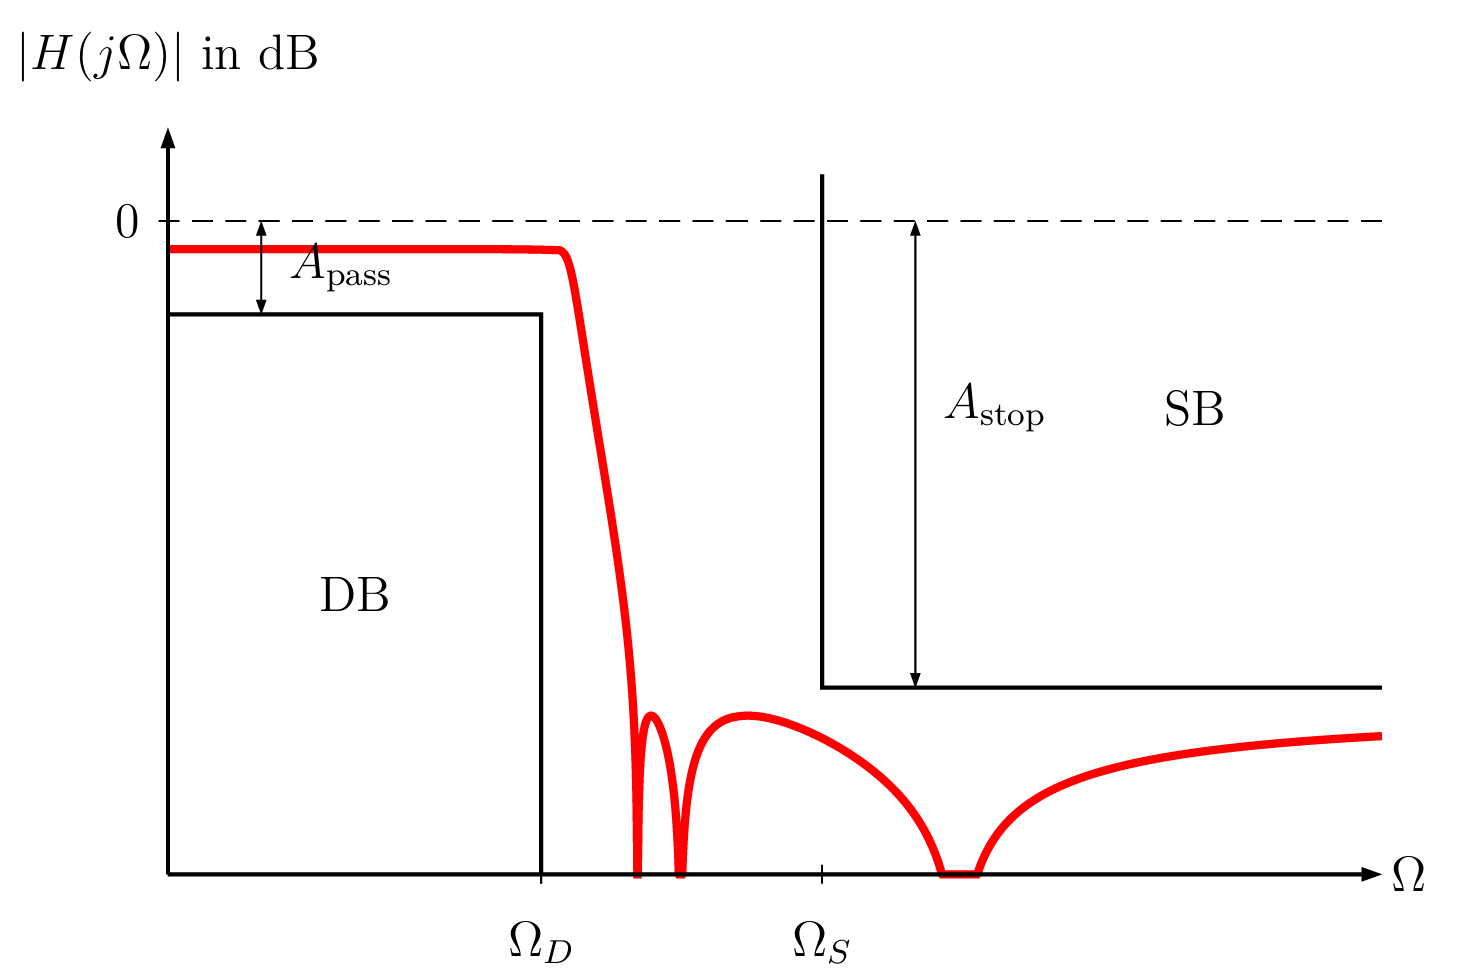
\includegraphics[width=\columnwidth]{images/filter_toleranzschema.png}
\end{minipage}
\hfill
\begin{minipage}[c]{0.48\columnwidth}
    Die Anforderungen an ein Filter werden häufig im \textbf{Toleranzschema beschrieben}. Dieses steht jeweils 'auf dem Kopf'.

    \begin{itemize}
        \item Im \textbf{Durchlassbereich (DB)} bestimmt der Stempel die maximal zulässige \textbf{Dämpfung} $A_{\max}$
        \item Im \textbf{Sperrbereich (SB)} bestimmt die Matritze die minimal nötige \textbf{Dämpfung} $A_{\min}$
    \end{itemize}
\end{minipage}

$$\boxed{ A_{\deci \bel}(\omega) = 10 \cdot \log \Biggl( \frac{1}{|H(\omega)|^2} \Biggr) = - 20 \cdot \log \bigl(|H(\omega)| \bigr) 
    \quad \textrightarrow\ \text{Dämpfung!} } $$


\subsubsection{Frequenznormierung}
\label{Frequenznormierung}
 
Um möglist kompakte \textbf{Tabellen} zu haben, wird auf Frequenzen normiert. Grundsätzlich kann auf eine beliebige Frequenz normiert
werden. Allerdings gilt grundsätzlich:

\begin{itemize}
    \item \textbf{HP / TP:} Normierung bezüglich \textbf{Grenzfrequenz} des Durchlassbereichs $\omega_r = \omega_D$
    \item BP / BS: Normierung bezüglich der Mittenfrequenz $\omega_r = \omega_m$
\end{itemize}
\vspace{0.2cm}

\begin{minipage}[c]{0.48\columnwidth}
    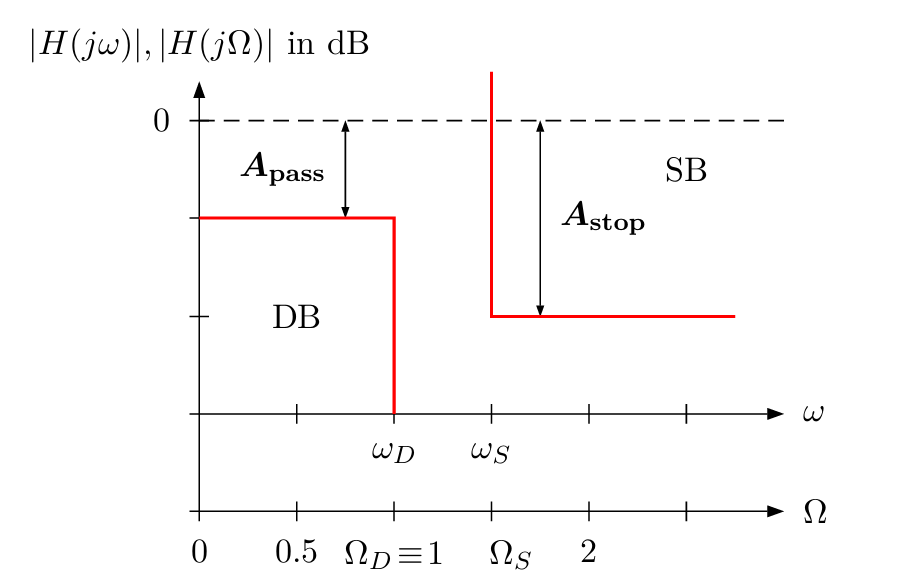
\includegraphics[width=\columnwidth]{images/filter_toleranzschema_frequenznormierung.png}
\end{minipage}
\hfill
\begin{minipage}[c]{0.48\columnwidth}
    \begin{center}
       \textbf{\myul{Normierte Grössen}}  
    \end{center}

    \vspace{-0.3cm}
    \begin{minipage}[c]{0.3\columnwidth}
        $$ \boxed{ S = \frac{s}{\omega_r}} $$
    \end{minipage}
    \hfill
    \begin{minipage}[c]{0.3\columnwidth}
        $$ \boxed{ \Omega = \frac{\omega}{\omega_r}} $$
    \end{minipage}
    \hfill
    \begin{minipage}[c]{0.3\columnwidth}
        $$ \boxed{ \sigma' = \frac{\sigma}{\omega_r}} $$ 
    \end{minipage}

    \vspace{0.2cm}
    \textbf{Entnormierung:} Jeweils $S$ in der normierten Funktion durch $\frac{s}{\omega_r}$ ersetzen.
\end{minipage}


\subsection{Ideales Tiefpassfilter}{297}

\begin{minipage}[c]{0.48\columnwidth}
    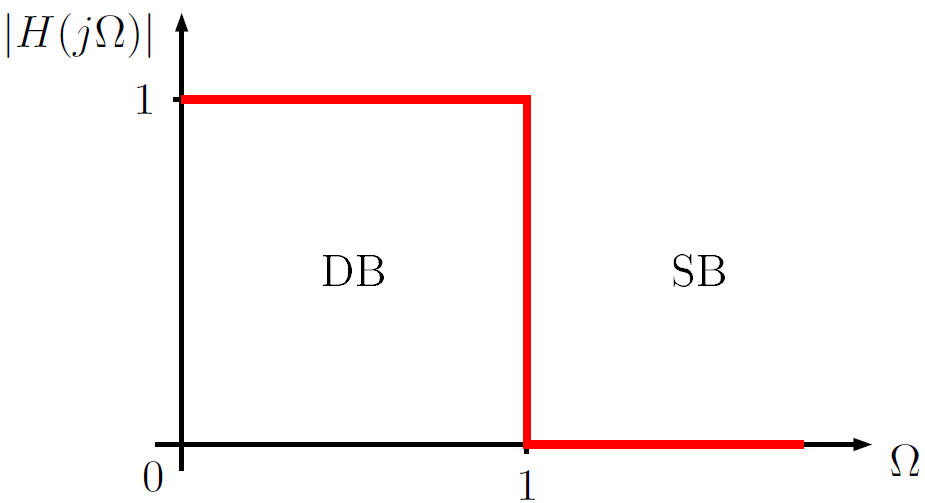
\includegraphics[width=\columnwidth]{images/filter_toleranzschema_idealer_tiefpass.png}

    \begin{itemize}
        \item DB: keine Dämpfung
        \item SB: kein Ausgangssignal
    \end{itemize}
\end{minipage}
\hfill
\begin{minipage}[c]{0.42\columnwidth}
    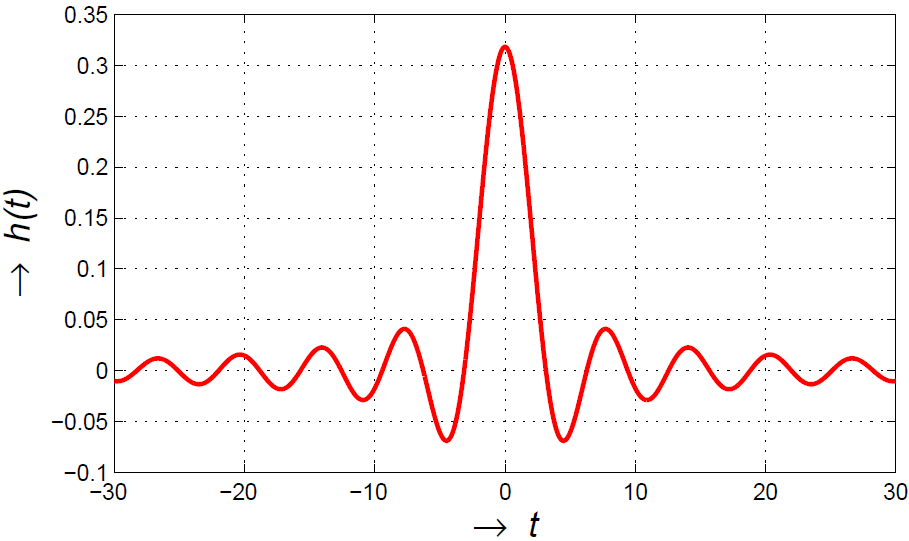
\includegraphics[width=\columnwidth]{images/filter_impulsantwort_idealer_tiefpass.png}
    
    \begin{itemize}
        \item Akausale Impulsantwort $h(t)$
    \end{itemize}
\end{minipage}

\vspace{0.2cm}
\textrightarrow\ Ideales Tiefpass ist physikatisch nicht realisierbar. \textrightarrow\ \textbf{Approximationen}


\subsection{Amplitudengang mit char. Funktion $K(\Omega^2)$}
\label{Amplitudengang mit char. Funktion}

Um Wurzelausdrücke zu vermeiden, wird der folgenden Ansatz verwendet
$$ \boxed{ | H(\jimg \Omega) |^2 = \frac{1}{1 + K(\Omega^2)}} $$

Im Fall des (idealen) Tiefpasses gilt für die charakteristische Funktion $K(\Omega^2)$

\begin{tabular}{l r l l}
    Durchlassbereich (DB)   & $0 \leq K(\Omega^2) \ll 1$    & für $0 \leq \Omega < 1$   & \textrightarrow\ $| H(\jimg \Omega) |^2 \approx 1$ \\
    Sperrbereich (SB)       & $K(\Omega^2) \gg 1$           & für $ \Omega > 1$         & \textrightarrow\ $| H(\jimg \Omega) |^2 \approx 0$ \\   
\end{tabular}



\subsection{Standard-Filtertypen -- Überblick}
\label{Standard-Filtertypen}

\begin{outline}
    \1 \textbf{Kritisch-gedämpfte Filter}
        \2[+] \textbf{Kein Rippel} im Durchlass- und Sperrbereich
        \2[+] Kein Überschwingen bei Impuls- und Sprungantwort
        \2[-] Braucht \textbf{hohe Ordnung} für steilen Übergang von Durchlass- zu Sperrbereich
        \2    Kaskadierung von $n$ wirkungsfreien, identischen Filtern 1. Ordnung
        \2    Bei $\Omega = 1$ \textrightarrow\ Dämpfung von $3 \, \deci \bel$
        \2    Steilheit: $- n \cdot 20 \, \deci \bel /$ Dekade
        \2    Allpolfiler: $n$ Pole am gleichen Ort in der LHE

    \1 \textbf{Butterworth}
        \2[+] \textbf{Kein Rippel} im Durchlass- und Sperrbereich
        \2[+] Im Durchlassbereich ist der Amplitudengang \textbf{maximal flach}
        \2[-] Überhöhung in der Gruppenlaufzeit der Grenzfrequenz
        \2[-] Braucht \textbf{hohe Ordnung} für steilen Übergang von Durchlass- zu Sperrbereich
        \2    Bei $\Omega = 1$ \textrightarrow\ Dämpfung von $3 \, \deci \bel$
        \2    Steilheit: $- n \cdot 20 \, \deci \bel /$ Dekade
        \2    Allpolfiler: Pole auf Einheitskreis mit Abstand $\frac{\pi}{n}$ 

    \1 \textbf{Tschebyscheff-\uproman{1}}
        \2[+] Schon für kleine Ordnungen \textbf{relativ steil} im Übergang von Durchlass- und Sperrbereich
        \2[-] \textbf{Rippel} im \textbf{Durchlassbereich} (abhängig von Ordnung $n$)
        \2[-] Keine konstante Gruppenlaufzeit (wellig)
        \2    Bei $\Omega = 1$ \textrightarrow\ Dämpfung abhängig von Rippelfaktor $e$
        \2    Steilheit: $- n \cdot 20 \, \deci \bel /$ Dekade
        \2    Allpolfiler: Pole auf einer Ellipse

    \1 \textbf{Tschebyscheff-\uproman{2}}
        \2[+] Schon für kleine Ordnungen \textbf{relativ steil} im Übergang von Durchlass- und Sperrbereich
        \2[-] \textbf{Rippel} im \textbf{Sperrbereich} (abhängig von Ordnung $n$)
        \2[-] Relativ konstante Gruppenlaufzeit
        \2    Bei $\Omega = 1$ \textrightarrow\ Dämpfung abhängig von Rippelfaktor $e$
        \2    Steilheit: $- n \cdot 20 \, \deci \bel /$ Dekade
        \2    Kein Allpolfilter

    \1 \textbf{Cauer}
        \2[+] Steilster Übergang von Durchlass- zu Sperrbereich
        \2[-] \textbf{Rippel} in \textbf{Durchlassbereich und Sperrbereich} (abhängig von Ordnung $n$)
        \2    \textbf{Kombination aus Tschebyscheff-\uproman{1} und Tschebyscheff-\uproman{2}}
        % \2    Steilheit: $- n \cdot 20 \, \deci \bel /$ Dekade
        \2    Kein Allpolfilter

    \1 \textbf{Bessel}
        \2[+] \textbf{Flachster Übergang} von Durchlass- und Sperrbereich von allen Filtern
        \2[+] Konstante Gruppenlaufzeit
        \2[-] Für steile Filter im Durchlass- und Sperrbereich nicht geeignet
        \2    Allpolfilter: Pole auf exzentrischen Kreisen in LHE
\end{outline}


\subsection{Gegenüberstellung der Filter-Approximationen} 

\scalebox{0.68}{
\begin{tabular}{|l|c|c|c|c|c|c|}
    \hline
    \multicolumn{1}{|c|}{} & \textbf{Krit. Gedämpft}                                            & \textbf{Butterworth}                                                    & \textbf{Tschebyscheff 1}                                        & \textbf{Tschebyscheff 2}                                       & \textbf{Cauer}                                                       & \textbf{Bessel}                                          \\ \hline
    \textbf{Allpolfilter}  & ja                                                                 & ja                                                                      & ja                                                              & nein                                                           & nein                                                                 & ja                                                       \\ \hline
    \textbf{Pol-Lage}      & \begin{tabular}[c]{@{}c@{}}reelle Achse\\ \textless 0\end{tabular} & \begin{tabular}[c]{@{}c@{}}Halbkreis\\ LHE\end{tabular}                 & \begin{tabular}[c]{@{}c@{}}Ellipse\\ LHE\end{tabular}           & LHE                                                            & \begin{tabular}[c]{@{}c@{}}Ellipse\\ LHE\end{tabular}                & \begin{tabular}[c]{@{}c@{}}exzentr.\\ Kreis\end{tabular} \\ \hline
    \textbf{NS-Lage}       & -                                                                  & -                                                                       & -                                                               & $\jimg \omega$-Achse                                           & $\jimg \omega$-Achse                                                 & -                                                        \\ \hline
    \textbf{DB}            & monoton                                                            & \begin{tabular}[c]{@{}c@{}}monoton\\ maximalflach\end{tabular}          & \begin{tabular}[c]{@{}c@{}}wellig\\ konst. Rippel\end{tabular}  & monoton                                                        & \begin{tabular}[c]{@{}c@{}}wellig\\ konst. Rippel\end{tabular}       & monoton                                                  \\ \hline
    \textbf{SB}            & streng                                                             & monoton                                                                 & monoton                                                         & \begin{tabular}[c]{@{}c@{}}wellig\\ konst. Rippel\end{tabular} & \begin{tabular}[c]{@{}c@{}}wellig\\ konst. Rippel\end{tabular}       & monoton                                                  \\ \hline
    \textbf{Phasengang}    & sehr gut                                                           & mittel                                                                  & schlecht                                                        & schlecht                                                       & wild                                                                 & bestmöglich                                              \\ \hline
\end{tabular}}


\subsubsection{Frequenzgänge / Lage der Pol- und Nullstellen}{334}

\begin{minipage}[c]{0.7\columnwidth}
    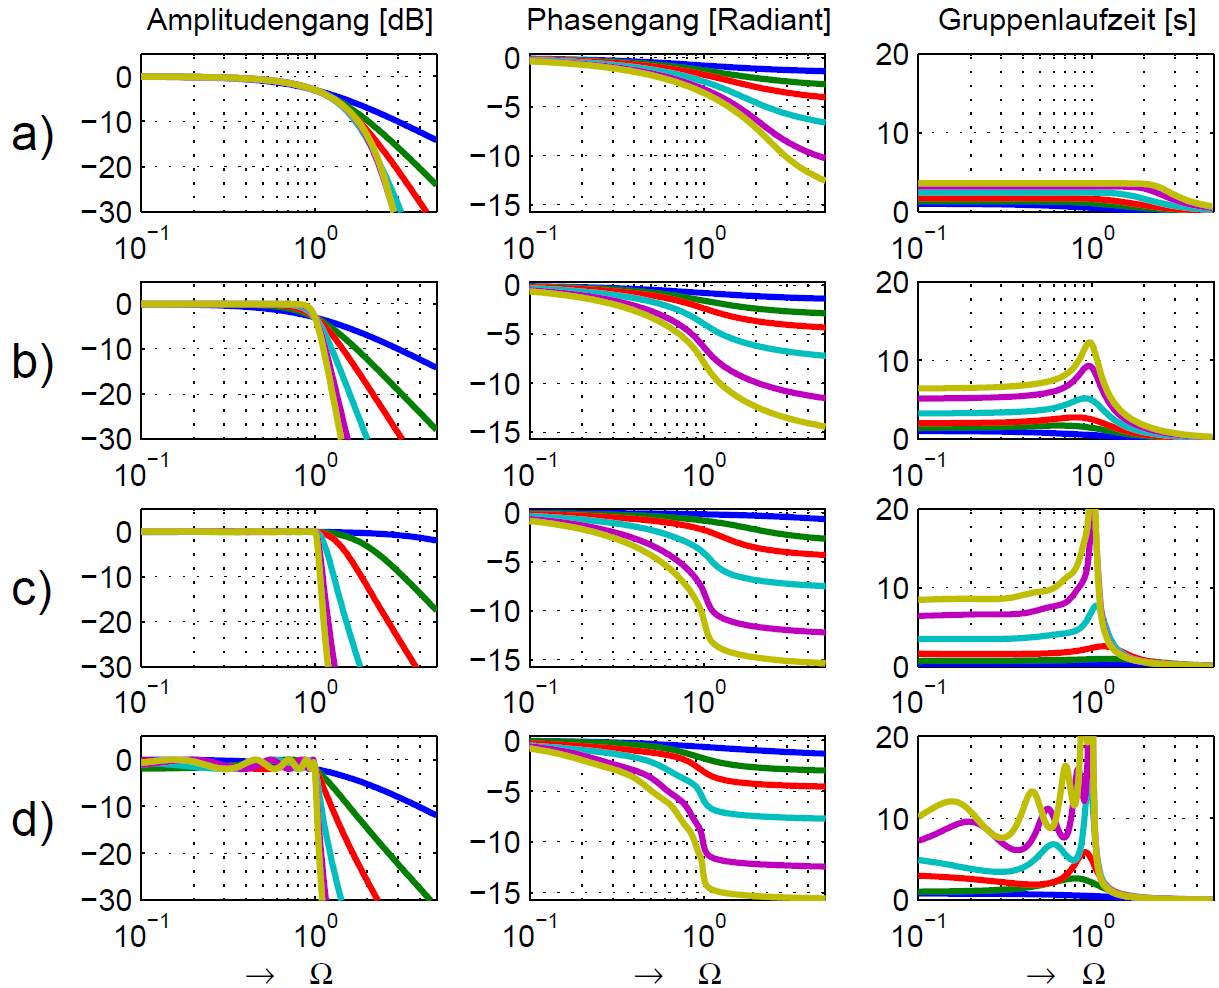
\includegraphics[width=\columnwidth]{images/filter_vergleich_frequenzgaenge.png}
\end{minipage}
\hfill
\begin{minipage}[c]{0.28\columnwidth}
    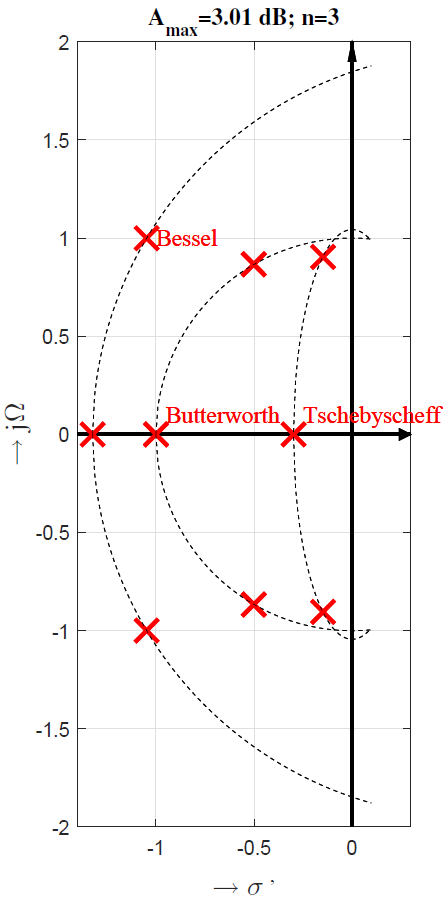
\includegraphics[width=\columnwidth]{images/filter_vergleich_pollagen.png}
\end{minipage}

\begin{tabular}{ll cc ll}
    a) & Bessel         & & & c) & Tschebyscheff ($0.1 \, \deci \bel$) \\
    b) & Butterworth    & & & d) & Tschebyscheff ($2 \, \deci \bel$) \\
\end{tabular}


\subsection{Vorgehen Filter dimensionieren / auslegen}

% TODO: fomrmatting of enumerate (#10 looks ugly)
\begin{enumerate}
    \item Gemäss Anforderungen geeigneten Filtertyp wählen (\textrightarrow\ \ref{Standard-Filtertypen})
    \item Toleranzschema gemäss Anforderungen erstellen \textbf{inkl. Normierung} (\textrightarrow\ \ref{Toleranzschema})
    \item Ordnung des Filters bestimmen (Formel oder \textbf{Nomogramm} \textrightarrow\ \ref{Nomogramme})
    \item Übertragungsfunktion bestimmen (\crd{\textrightarrow\ Tabelle: Skript S. 397, Anhang 7B})
    \item Implementierung mit LC-Filtern: Topologie wählen (\crd{\textrightarrow\ Skript S. 409, Anhang 7C})
    \item \textbf{Normierte} Bauteilwerte aus entsprechender Tiefpass-Tabelle herauslesen (Anhang 7C)
    \item \textbf{Falls nicht auf $\bm{\omega_r = \omega_{3 \, \deci \bel}}$ normiert wurde:} Normierte Werte auf $\Omega_{3 \, \deci \bel}$ korrigieren: \\
         \textrightarrow\ Division durch \cbl{Korrekturfaktor} aus Skript S. 401 Tabelle 7.8
    \item Komponenten mittels \textbf{Entnormierung} bestimmen (\textrightarrow\ \ref{Entnormierung Komponenten})
    \item \textbf{Entnormierung} der Frequenz (\textrightarrow\ \ref{Frequenznormierung})\\
        $\omega_{3 \, \deci \bel} = \text{\cbl{Korrekturfaktor}} \cdot \omega_r = \text{\cbl{Korrekturfaktor}} \cdot 2 \pi f_r $
    \item Frequenztransformation (bzw. Komponenten-Transformation) zu HP, BP oder BS durchführen (\textrightarrow\ \ref{Frequenztransformation})
\end{enumerate}


\subsection{Nomogramme}{393}
\label{Nomogramme}

Nomogramme können verwendet werden, um die \textbf{Ordnung eines Filters}  zu bestimmen.

\begin{minipage}[c]{0.42\columnwidth}
    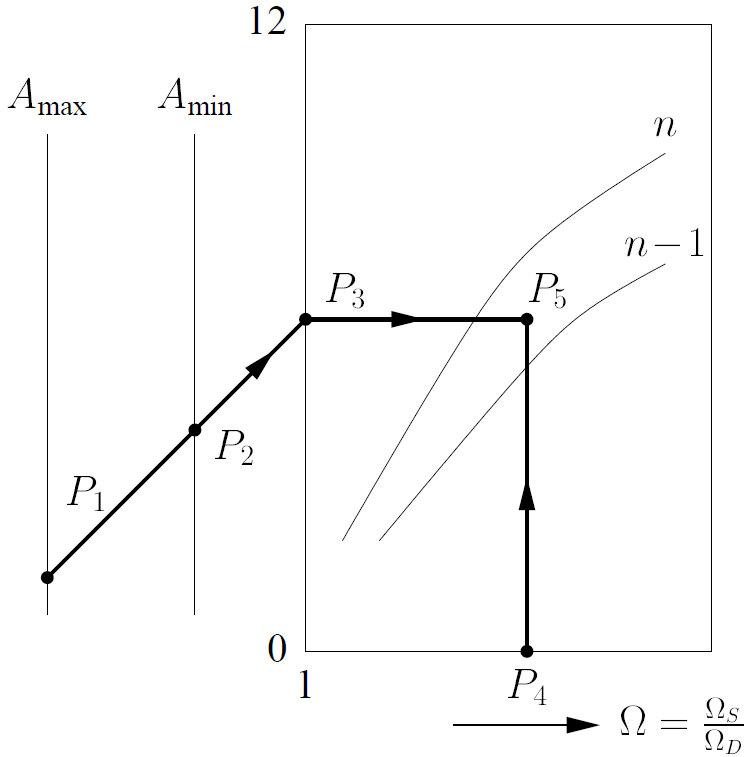
\includegraphics[width=\columnwidth]{images/filter_nomogramme.png}
\end{minipage}
\hfill
\begin{minipage}[c]{0.56\columnwidth}
    \begin{center}
        \textbf{\myul{Benutzung von Nomogrammen}}
    \end{center}
    
    \begin{enumerate}
        \item $P_1$: Verbindung von $A_{\max}$ zu $A_{\min}$
        \item $P_2$: Verlängerung von $P_1$ bis zum 'Diagramm-Rand'
        \item $P_3$: Horizontale Linie vom Rand in Diagramm hinein
        \item $P_4$: Bei $\Omega = \frac{\Omega_S}{\Omega_D} = \frac{\omega_S}{\omega_D} = \frac{f_S}{f_D}$ vertikale Linie ziehen
        \item $P_5$: Schnittpunkt: 'hochfahren' zur nächsten Kurve \textrightarrow\ Ordnung $n$ der Kurve ablesen
    \end{enumerate}
\end{minipage}


\subsection{LC-Filter: Entnormierung der Komponenten}
\label{Entnormierung Komponenten}

$$ \boxed{ L = \frac{L_{\rm norm}}{\omega_r} \cdot R_r}
\qquad \boxed{ C = \frac{C_{\rm norm}}{\omega_r \cdot R_r }}
\qquad \boxed{ R = R_{\rm norm} \cdot R_r } $$

\begin{center}
    \begin{tabular}{ll}
        $L_{\rm norm}$  & normierter Wert gemäss Skript, Anhang 7C \\
        $C_{\rm norm}$  & normierter Wert gemäss Skript, Anhang 7C \\
        $R_{\rm norm}$  & normierter Wert gemäss Skript, Anhang 7C \\
        $\omega_r$  & Frequenz, auf welche normiert wurde ($\omega_D$ oder $\omega_m$ gemäss \ref{Frequenznormierung}) \\
        $R_r$       & Tatsächlicher Wert von $R_2$ gemäss Topologie Skript S. 409
    \end{tabular}
\end{center}
    

    \end{layout}
\end{document}
